\chapter{L’implémentation}

%\section{Environnement de développement}
\section{Environnement de travail}
Durant la réalisation de ce projet, nous avons essayé d’utiliser différents
outils de développement, d’une part afin de rendre la tâche de la
réalisation plus facile, d’autre part pour que notre système soit robuste et
répond parfaitement a nos besoins , et que nos interfaces soient claires et
faciles à utiliser.
\subsection{Environnement logiciel}

\begin{comment}
	content...

\subsection{Front-end}
C’est le développement coté client autrement dit la
partie du code reçu par le client. On rappelle que le client désigne
un navigateur web.
On a choisi Flutter comme Framework pour développer la partie
front de notre application mobile.
Flutter est un framework de développement d’applications mobiles open source de Google. La principale raison de sa popularité est qu’il prend en charge la création 		   
d’applications multiplateformes. Flutter est également utilisé pour créer des apps interactives qui s’exécutent sur des pages web ou sur le bureau.
\end{comment}
\subsubsection{Editeur de texte : VS Code}
\begin{figure}[h]
	
\includegraphics[scale=0.4]{./Template LaTeX/Images/VSCode.jpg}
	\centering
	\caption{VS Code}
\end{figure}
VS Code (Visual Studio Code) est un éditeur de code source réalisé par Microsoft pour Win-
dows, Linux et macOS.Les fonctionnalités incluent la prise en charge du débogage, lacoloration
syntaxique, la saisie semi-automatique intelligente du code, les extraits de code, la refactorisation du
code et Gitintégré. Les utilisateurs peuvent modifier le thème,les raccourcis clavier,les préférences et
installer des extensions qui ajoutent des fonctionnalités supplémentaires.\newline Pour en savoir plus, veillez
visiter le lien : \href{https://en.wikipedia.org/wiki/VisualStudioCode}{https://en.wikipedia.org/wiki/VisualStudioCode}
\subsubsection{IDE : Android Studio}
\begin{figure}[h]
	
\includegraphics[scale=0.2]{./Template LaTeX/Images/Android_Studio_Icon_3.6.svg}
	\centering
	\caption{Android Studio}
\end{figure}
Android Studio est un environnement de développement pour développer des applications mobiles Android. Il est basé sur IntelliJ IDEA et utilise le moteur de production Gradle. Il peut être téléchargé sous les systèmes d'exploitation Windows, macOS, Chrome OS et Linux.
\newline Pour en savoir plus, veillez
visiter le lien : \href{https://en.wikipedia.org/wiki/AndroidStudio.}{https://en.wikipedia.org/wiki/AndroidStudio.}
\subsubsection{Git}
\begin{figure}[h]
	
\includegraphics[scale=0.3]{./Template LaTeX/Images/Git-Icon.png}
	\centering
	\caption{Git}
\end{figure}
Git est un système de contrôle de version distribué gratuit et Open Source conçu pour gérer des
petits projets aux très grands projets avec rapidité et efficacité. C'est un logiciel libre créé par
Linus Torvalds, auteur du noyau Linux, et distribué selon les termes de la licence publique
générale GNU version 2 \href{https://edu.casio.com/support/fr/gplv2.html}{GPLv2}. Depuis 2016, il s’agit du logiciel de gestion de versions le
plus populaire. Git possède deux structures de données : une base d'objets et un cache de
répertoires. Il existe quatre types d'objets :
\begin{itemize}[label=$\ast$]
	
	\item  l'objet \textbf{blob} (pour binary large object désignant un ensemble de données brutes) qui
	représente le contenu d'un fichier ;
	\item l'objet \textbf{tree} (mot anglais signifiant arbre) qui décrit une arborescence de fichiers. Il est
	constitué d'une liste d'objets de type blobs et des informations qui leur sont associées
	telles que le nom du fichier et les permissions. Il peut contenir récursivement d'autres
	objets trees pour représenter les sous-répertoires ;
	\item l'objet \textbf{commit} (résultat de l'opération du même nom signifiant « valider une transaction
	») qui correspond à une arborescence de fichiers (tree) enrichie de métadonnées comme
	un message de description, le nom de l'auteur, etc. Il pointe également vers un ou
	plusieurs objets commit parents pour former un graphe d'historiques ;
	\item l'objet \textbf{tag} qui est une manière de nommer arbitrairement un commit
	spécifique pour l'identifier plus facilement. Il est en général utilisé pour marquer certains
	commits.
	
\end{itemize}


veillez
visiter le lien :
\href{https://git-scm.com/s}{https://git-scm.com/s}
\subsubsection{Le SGBD Firebase}
\begin{figure}[h]
	
\includegraphics[scale=0.1]{./Template LaTeX/Images/firebase.png}
	\centering
	\caption{Firebase}
\end{figure}
Firebase est une plateforme d’hébergement pour n’importe quel type d’application (mobiles,
Web, etc.) qui fournit aux développeurs une pléthore d'outils et de services pour les aider à
développer des applications de haute qualité, à élargir leur base d'utilisateurs et à générer
davantage de profits. Il propose d'héberger en NoSQL et en temps réel des bases de données,
du contenu, de l'authentification sociale (Google, Facebook, Twitter et Github) et des notifications, ou encore des services tels que par exemple un serveur de communication en
temps réel [1].
Lancé en 2011 sous le nom d'Envolve, par Andrew Lee et par James Templin, le service est
racheté par Google en octobre 2014. Il appartient aujourd'hui à la maison mère de Google :
Alphabet (maison-mère de groupe qui regroupe une majorité des activités du groupe comme
YouTube, Android, la recherche et les publicités). L'objectif premier de Firebase est de vous
libérer de la complexité de création et de la maintenance d'une architecture serveur, tout en vous
garantissant une scalabilité (capacité de l’application à s'adapter à un changement d'ordre de
grandeur de la demande, en particulier sa capacité à maintenir ses fonctionnalités et ses
performances en cas de forte demande) à toute épreuve (plusieurs milliards d'utilisateurs) et une
simplicité dans l'utilisation. Pour cela, Firebase a été décomposée en plusieurs produits
extrêmement riches et adaptés au monde du mobile, dont la liste suivante :
\setcounter{secnumdepth}{5}
\paragraph{Firebase Realtime Database :\newline}


 Firebase Realtime Database est une base de données NoSQL hébergée dans le cloud qui vous
permet de stocker et de synchroniser des données entre vos utilisateurs en temps réel [1], [2].
Realtime Database est vraiment juste un gros objet JSON que les développeurs peuvent gérer
en temps réel.
La synchronisation en temps réel permet à vos utilisateurs d'accéder facilement à leurs données
depuis n'importe quel appareil, que ce soit sur le Web ou sur un appareil mobile. La base de
données en temps réel permet également à vos utilisateurs de collaborer les uns avec les autres.
Un autre gros avantage de Realtime Database est qu'elle est livrée avec des SDK mobiles et
Web, vous permettant de créer vos applications sans avoir besoin de serveurs. Lorsque vos
utilisateurs sont hors ligne, les SDK de base de données en temps réel utilisent le cache local
sur l'appareil pour servir et stocker les modifications. Lorsque l'appareil est en ligne, les données
locales sont automatiquement synchronisées.
\paragraph{Firebase Authentication :\newline}
Firebase Authentication fournit des services backend, des SDK faciles à utiliser et des
bibliothèques d'interfaces utilisateur prêtes à l'emploi pour authentifier les utilisateurs de votre
application [1], [2].
Vous pouvez authentifier les utilisateurs de votre application à l'aide des méthodes suivantes :
\begin{itemize}[label=$\ast$]
	\item Email et mot de passe
	\item Numéro de téléphone
	\item Compte Google
	\item Compte Facebook
	\item Compte Twitter
	\item Etc.
\end{itemize}
L'utilisation de Firebase Authentication facilite la création de systèmes d'authentification
sécurisés, tout en améliorant l'expérience de connexion et d'intégration pour les utilisateurs
finaux.
\paragraph{Firebase Cloud Messaging (FCM) :\newline}
Firebase Cloud Messaging (FCM) fournit une connexion fiable et à faible consommation de
batterie entre votre serveur et vos périphériques, vous permettant d'envoyer et de recevoir
gratuitement des messages et des notifications sur iOS, Android et sur le Web [1], [2]. Vous
pouvez envoyer des messages de notification (limite de 2 Ko) et des messages de données
(limite de 4 Ko).
En utilisant FCM, vous pouvez facilement cibler les messages en utilisant des segments
prédéfinis ou créer les vôtres, en utilisant les données démographiques et comportementales.
Vous pouvez envoyer des messages à un groupe d'appareils abonnés à des rubriques
spécifiques, ou vous pouvez obtenir des informations aussi détaillées qu'un seul appareil.
FCM peut envoyer des messages instantanément, ou à un moment ultérieur dans le fuseau
horaire local de l'utilisateur. Vous pouvez envoyer des données d'application personnalisées,
telles que la définition des priorités, des sons et des dates d'expiration, ainsi que le suivi des
événements de conversion.
\paragraph{Cloud Firestore :\newline}
Cloud Firestore est une base de données de documents NoSQL qui vous permet de facilement
stocker, synchroniser et interroger des données pour vos applications mobiles et Web à l'échelle
mondiale [1], [2]. Bien que cela puisse ressembler à quelque chose de similaire à la base de
données en temps réel, Firestore apporte beaucoup de nouvelles choses à la plateforme qui est
en fait quelque chose de complètement différent de Realtime Database.
Là où Realtime Database stocke des données sous la forme d'un arbre JSON géant, Cloud
Firestore adopte une approche beaucoup plus structurée. Firestore conserve ses données dans des objets appelés documents. Ces documents sont constitués de paires clé-valeur et peuvent
contenir n'importe quel type de données, depuis les chaînes jusqu'aux données binaires en
passant par des objets qui ressemblent à des arbres JSON (Firestore l'appelle des maps). Les
documents, à leur tour, sont regroupés en collections.
La base de données Firestore peut se composer de plusieurs collections qui peuvent contenir
des documents pointant vers des sous-collections. Ces sous-collections peuvent à nouveau
contenir des documents qui pointent vers d'autres sous-collections, et ainsi de suite.
Vous pouvez créer des hiérarchies pour stocker les données associées et récupérer facilement
les données dont vous avez besoin à l'aide de requêtes. Toutes les requêtes peuvent évoluer en
fonction de la taille de votre jeu de résultats. Votre application est donc prête à évoluer depuis
le premier jour.
\subsubsection{SGBD MariaDB}

\begin{figure}[h]
	
\includegraphics[scale=0.5]{./Template LaTeX/Images/logo-mariadb-500px.png}
	\centering
	\caption{SGBD MariaDB}
\end{figure}
Un gestionnaire de base de données libre.
ce projet est assurée par la fondation Maria DB, et sa
maintenance par la société Monty Program AB, créateur du
projet, il confère au logiciel l'assurance de rester libre. MariaDB a
plusieurs et différentes versions. Ells s'articulent sur le code
source de MySQL de la version 5.1 aux versions plus récentes
(comme la 5.6 fin 2012). Un serveur qui stocke les données dans
des tables séparées plutôt que de tout rassembler dans une seule
table. Du coup il améliore la rapidité et la souplesse de
l'ensemble.

\subsubsection{Logiciel de modélisation: Modelio}
\begin{figure}[h]
	
\includegraphics[scale=0.5]{./Template LaTeX/Images/modelio.jpg}
	\centering
	\caption{Modelio}
\end{figure}
\newpage
Modelio est un logiciel open source et multiplateforme permettant, entre autres, la modélisation
UML et Business Process Model and Notation (BPMN). Pour en savoir plus, veuillez visiter le lien
\href{https://www.modelio.org/about-modelio/features.html.}{https://www.modelio.org/about-modelio/features.html.}
Sans doute, les logiciels de modélisation UML sont nombreux, à savoir, Visual Paradigm, Eclipse
Papyrus, StarUML, PowerDesigner, Umbrello, etc. Vu que les diagrammes UML que nous voulons
réaliser sont disponibles dans tous ces logiciels, il n’y avait pas en effet un choix à argumenter car
tous les choix étaient satisfaisants. Mais, de façon subjective, nous pouvons préciser que l’avantage de
Modelio dans notre contexte est le fait que je m’y suis déjà habitués. Les diagrammes que nous avons
réalisés avec Modelio sont ceux mentionnés ci-après.


\subsubsection{Motifs d’architecture logicielle}
\paragraph{MVC \newline}
Le patron de conception MVC est l’une des bases du Framework
laravel, c’est-à-dire modèle-vue- contrôleur. L’interaction avec la
base de données est assurée par le Model, les regroupe, traite et
gère les données.
Pour faire afficher ce que le modèle renvoie on fait appelle a la vue .
elle s’occupe d’autre part de la réception de toute interaction de
l’utilisateur. Ce sont ces actions-là que le contrôleur gère.
Ainsi que l’échange entre le modèle et la vue. Il intercepte toutes les
activités de utilisateur et, en fonction de ces activités, il actionne les
changements à effectuer sur l'application.
Les composants sont séparés en ces trois catégories précédentes
permet une clarté de architecture des dossiers et simplifie
grandement la tâche aux développeurs.
\begin{figure}[h!]
	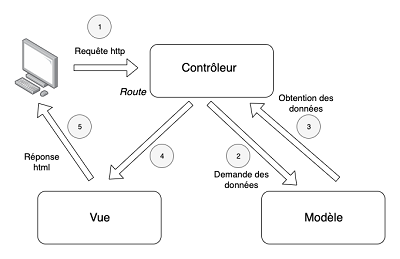
\includegraphics[width=15cm, height=6cm]{./Template LaTeX/Images/Modèle-vue-contrôleur_(MVC)_-_fr.png}
	\caption{MVC}
	\label{fig:birds}
\end{figure}
\newline \newline \newline
\textbf{Les fichiers sont organisés comme suit :}
\begin{enumerate}
	\item [-] \textbf{Route (Dispatcher) : }il contient les définitions des chemins d’entrées pour l’utilisateur,
	autrement dit les URI possibles et les dirige sur la classe définit dans
	le contrôleur qui doit traiter l’information.
	\item [-] \textbf{ Modèle : }pour chaque table de notre base de données que l’on veut
	utiliser pour notre application, il faut créer un modèle pour chacun.
	Ainsi nous avons ici un modèle de notre application. Il permet de
	décrire la méthode d’accès aux données de la base, tous cela à
	travers un objet définit par ORM Eloquent(Object-Relational
	Mapping).
	\item [-] \textbf{Contrôleur : } il permet de récupérer les informations du modèle et de l’envoyer
	vers la vue pour la mise en forme.
	\item [-] \textbf{Vue : } la vue réceptionne la réponse qui est envoyée par le
	contrôleur .\newline
\end{enumerate}
\subsubsection{Serveur Web : Amazon Web Services (AWS)}
\begin{figure}[h]
	
\includegraphics[scale=0.3]{./Template LaTeX/Images/512px-Amazon_Web_Services_Logo.svg.png}
	\centering
	\caption{Amazon Web Services (AWS)}
\end{figure}
Amazon Web Services (AWS) est la plateforme cloud la plus complète et la plus largement adoptée au monde. Elle propose plus de 200 services complets issus de centres de données du monde entier. Des millions de clients (dont certaines des startups les plus dynamiques au monde, de très grandes entreprises et des agences fédérales de premier plan) utilisent AWS pour réduire leurs coûts, gagner en agilité et innover plus rapidement.

\subsection{Conception}
\subsubsection{Langage de modélisation : UML}
\begin{figure}[h]
	
\includegraphics[scale=1]{./Template LaTeX/Images/formation-uml-analser-concevoir.png}
	\centering
	\caption{UML}
\end{figure}
On a utilisé UML comme langage de modélisation.
Langage de modélisation unifié UML (Unified modeling Langage) un
consiste a modéliser une application logicielle d'une façon standard
dans le cadre de conception orientée objet.
UML consiste a couvrir le cycle de vie d'un logiciel depuis la
spécification des besoins jusqu'au codage en offrant plusieurs
moyens de description et de modélisation des acteurs.





\section{Choix des outils de travail }
\subsection{Langages utilisés}
\subsubsection{Dart}
\begin{figure}[h]
	
\includegraphics[scale=0.4]{./Template LaTeX/Images/Dart_programming_language_logo.svg.png}
	\centering
	\caption{Dart}
\end{figure}
Dart est un langage de programmation open source à usage général. Il est initialement développé par Google. Dart est un langage orienté objet avec une syntaxe de C-style. Il prend en chargent les concepts de programmation tels que les interfaces, les classes, contrairement aux autres langages de programmation, Dart ne prend pas en charge les tableaux.
Les collections Dart peuvent être utilisées pour répliquer des structures de données telles que des tableaux, des génériques et un typage facultatif.
\newline Pour en savoir plus, veillez
visiter le lien : \href{https://www.tutorialspoint.com/flutter/flutter_introduction_to_dart_programming.htm}{https://www.tutorialspoint.com/flutter/dart}
\subsubsection{PHP}
\begin{figure}[h]
	
\includegraphics[scale=0.3]{./Template LaTeX/Images/PHP-logo.svg.png}
	\centering
	\caption{PHP}
\end{figure}
PHP est un langage de script utilisé le plus souvent côté serveur : dans cette architecture, le serveur interprète le code PHP des pages web demandées et génère du code (HTML, XHTML, CSS par exemple) et des données (JPEG, GIF, PNG par exemple) pouvant être interprétés et rendus par un navigateur web. PHP peut également générer d'autres formats comme le WML, le SVG et le PDF.

Il a été conçu pour permettre la création d'applications dynamiques, le plus souvent développées pour le Web. PHP est le plus souvent couplé à un serveur Apache bien qu'il puisse être installé sur la plupart des serveurs HTTP tels que IIS ou nginx. Ce couplage permet de récupérer des informations issues d'une base de données, d'un système de fichiers (contenu de fichiers et de l'arborescence) ou plus simplement des données envoyées par le navigateur afin d'être interprétées ou stockées pour une utilisation ultérieure.
\newline Pour en savoir plus, veillez
visiter le lien : \href{https://fr.wikipedia.org/wiki/PHP}{https://fr.wikipedia.org/wiki/PHP}
\subsection{Frameworks utilisés}

\subsubsection{Flutter}
\begin{figure}[h]
	
\includegraphics[scale=0.3]{./Template LaTeX/Images/Flutter.png}
	\centering
	\caption{Flutter}
\end{figure}
Flutter est un framework de développement d’applications mobiles open source de Google. La principale raison de sa popularité est qu’il prend en charge la création 		   
d’applications multiplateformes. Flutter est également utilisé pour créer des apps interactives qui s’exécutent sur des pages web ou sur le bureau.\newline
\textbf {- Les caractéristiques de Flutter :}


\begin{enumerate}
	\item Base de code unique pour Android et iOS
	\item Fonction de rechargement à chaud (hot reload)
	\item Open-source et par Google
	\item Programmation Dart \newline \newline \newline
\end{enumerate}


\textbf {- Architecture d’une application Flutter :} 
\begin{figure}[h!]
	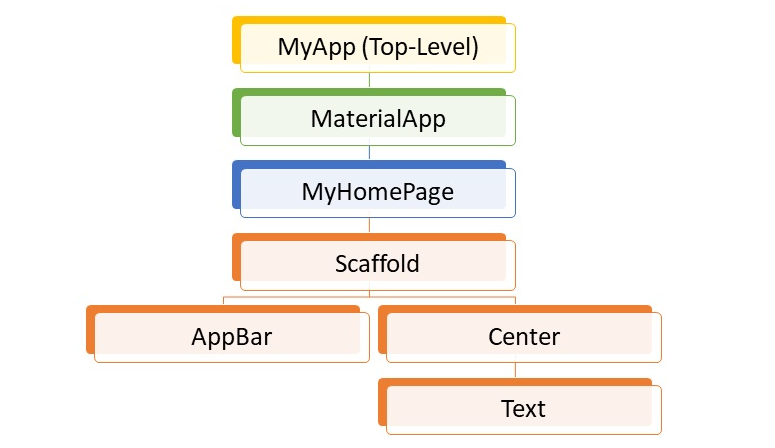
\includegraphics[width=450px,height=250px]{./Template LaTeX/Images/Flutter_architect.png}
	\caption{Architecture d’une application Flutter.}
	\label{fig:birds}
\end{figure}
\newpage
\subsubsection{Laravel}
\begin{figure}[h]
	
\includegraphics[scale=0.2]{./Template LaTeX/Images/462px-Laravel.svg.png}
	\centering
	\caption{Laravel}
\end{figure}
Laravel est un framework web open-source écrit en  \href{https://fr.wikipedia.org/wiki/PHP}{PHP} respectant le principe modèle-vue-contrôleur et entièrement développé en programmation orientée objet. Laravel est distribué sous \href{https://fr.wikipedia.org/wiki/Licence_MIT}{licence MIT}, avec ses sources hébergées sur 
\href{https://fr.wikipedia.org/wiki/GitHub}{GitHub}.\newline\newline
\textbf {- Les caractéristiques de Laravel :}

\begin{figure}[h!]
	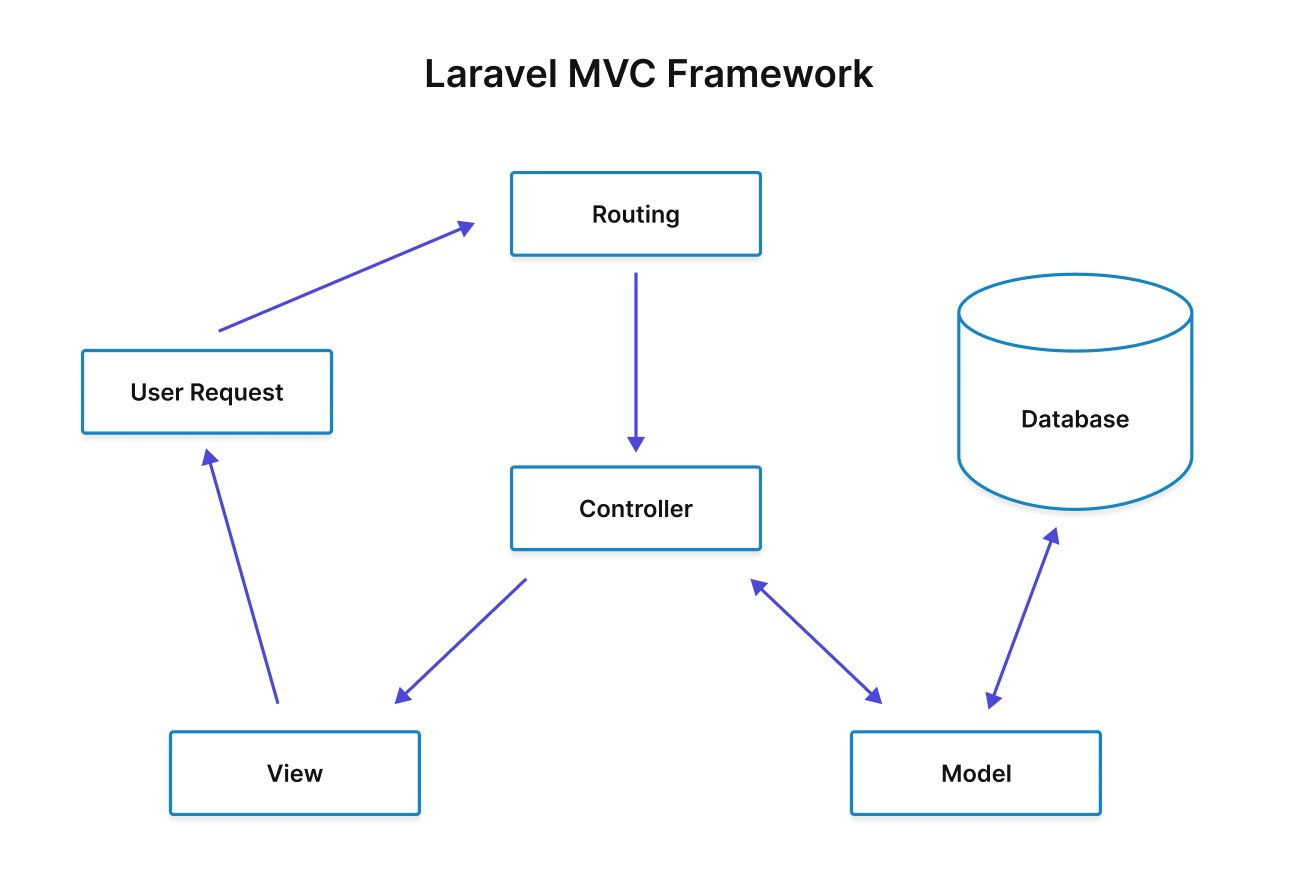
\includegraphics[width=500px,height=200px]{./Template LaTeX/Images/Laravel-MVC-framework.jpg}
	\caption{Architecture de Laravel}
	\label{fig:birds}
\end{figure}
\newpage
\section{Implémentation}
\subsection{Etape de réalisation}
Pour réaliser notre système, il y a des étapes à élaborer dans l’ordre suivant :
\begin{itemize}[label=$\ast$]
	\item \textbf{Conception de la base de données :} La conception d’une base de données est la
	première étape. Le choix des algorithmes et de l’approche de travail exige l’utilisation
	d’une base de données spécifique (en fonction du système à développer).
	\item \textbf{Extraction des données :}  On va utiliser notre SGBD Firebase ainsi que notre base de
	données en interaction avec l’application pour extraire des informations. Firebase est
	conçu avec des fonctionnalités et des requêtes de sélection de données assez spécifique
	et facile à utiliser.
	\item \textbf{Conception et développement du front-end et du back-end :} 
	Cette étape consiste à
	détailler la conception coté client et coté serveur. Il s’agit de mettre en place un design
	ergonomique, simple et attractif répondant aux exigences du système. Le choix d’un
	serveur d’application adéquat aux fonctionnalités et aux données est une étape
	fondamentale pour le bon fonctionnement de l’application.
	\item \textbf{Développement de back-end :} On commence par le développement de l’application coté
	serveur, dans notre cas avec \textbf{Laravel}. C’est la partie du code exécuté sur le serveur afin
	de vérifier le comportement des fonctionnalités de base du système.
	\item \textbf{Développement front-end :} On développe la partie client en interaction avec le serveur.
	C’est la conception de l'interface graphique utilisateur. En effet, il s'agit de la partie
	visible de l'application, destinée à être manipulée par un tiers.
\end{itemize}
\subsection{Interfaces Homme/Machine}
Dans ce qui suit, nous présentons quelques écrans de notre produit final des applictions CADORIM et Cadorim service.
\subsubsection{Application CADORIM}
\begin{itemize}[label=$\ast$]
		\item \textbf{Première interface :} L'utilisateur du Cadorim avant d'être invite à consulter les services de l'application, doit 
			choisies leur langue avant qu'il pass a l'interface suivante.
			
			\begin{figure}[!ht]
				\centering
				\begin{subfigure}{0.3\textwidth}
					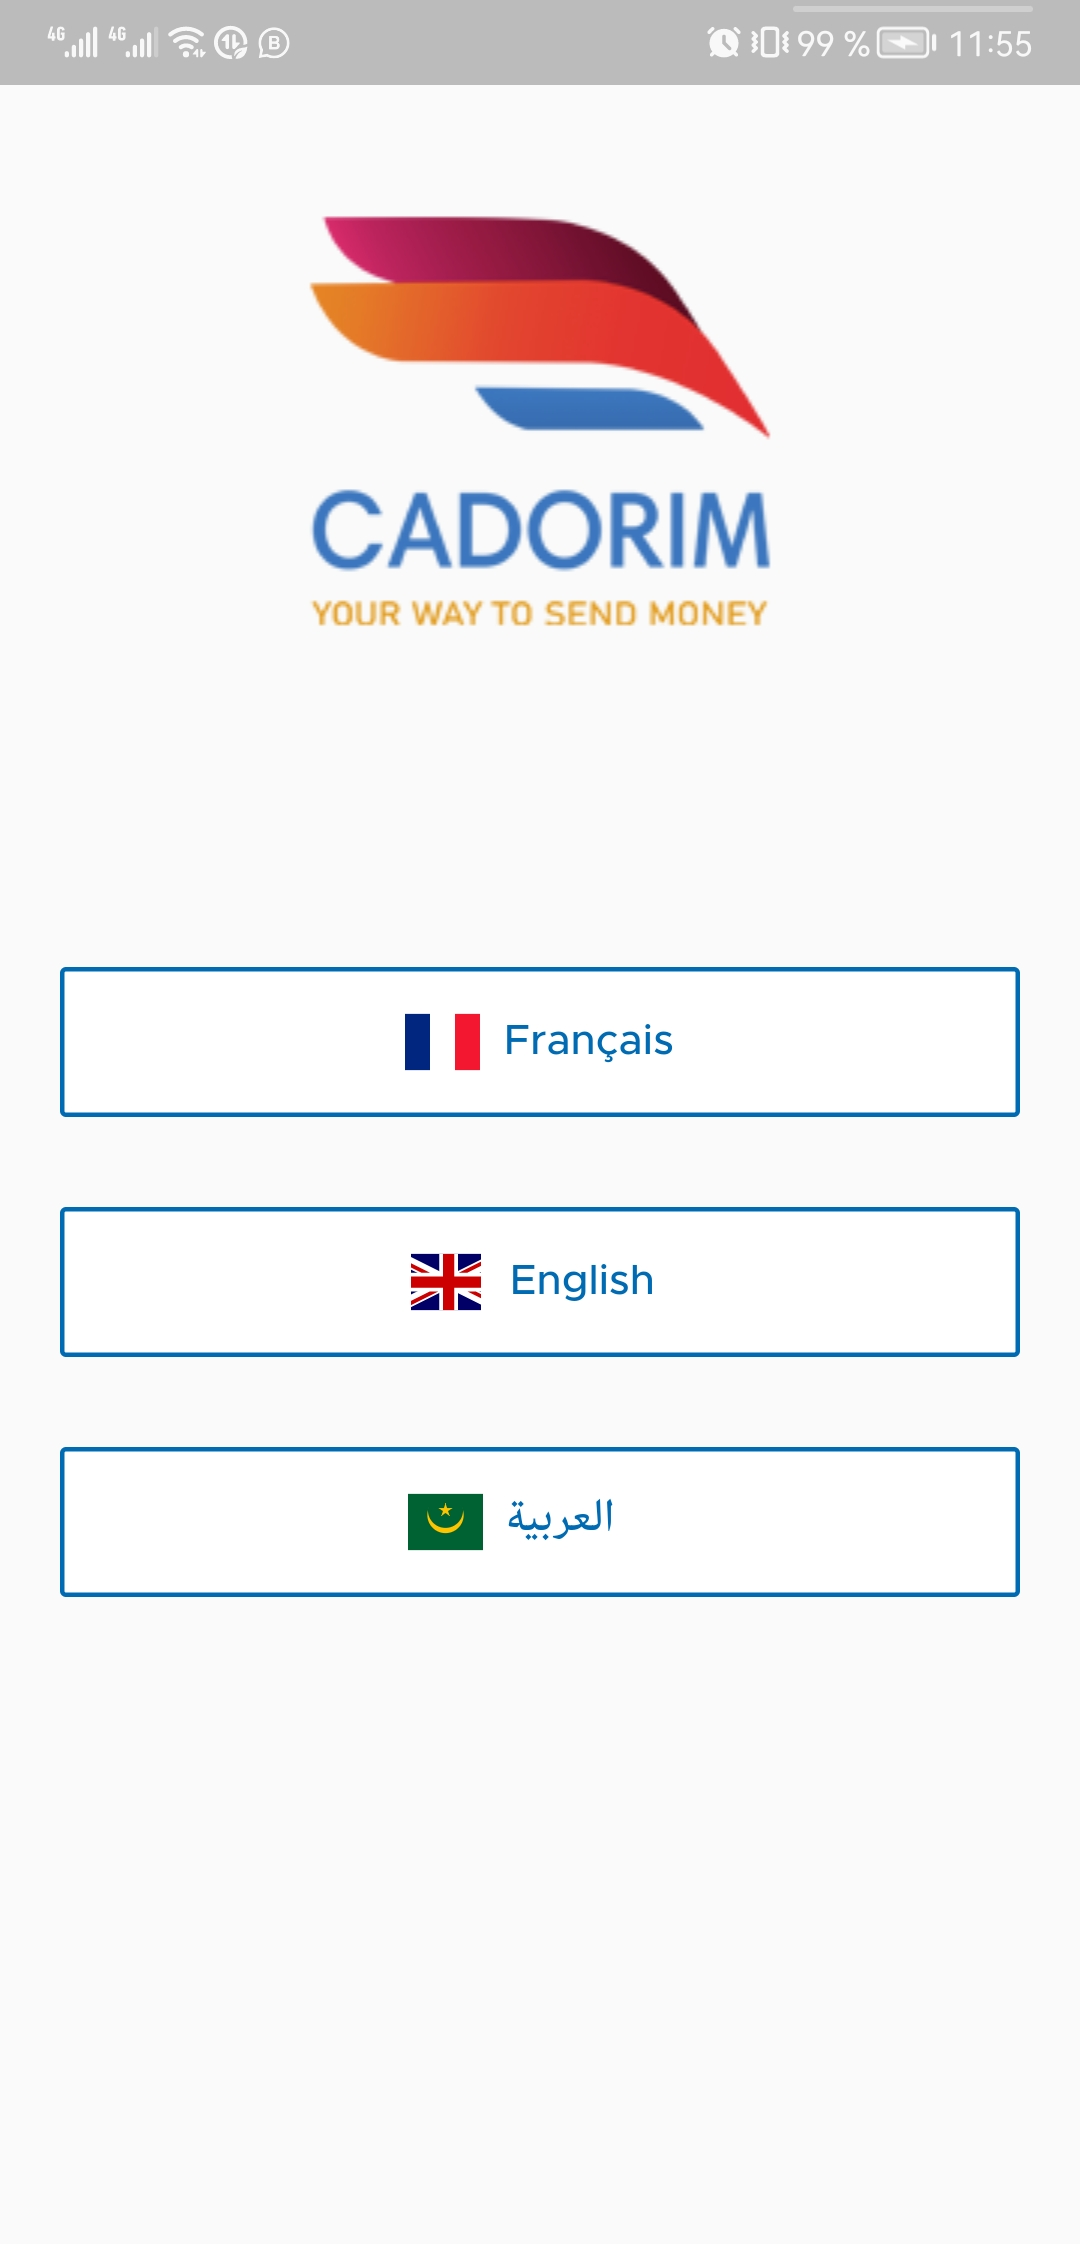
\includegraphics[width=\hsize, valign=m ]{./Template LaTeX/Images/1.jpg}
					\caption{Choix de langue}
					\label{fig.SICAPI}
				\end{subfigure}
				\qquad\tikz[baseline=-\baselineskip]\draw[ultra thick,->] (0,0) -- ++ (1,0);\qquad
				\begin{subfigure}{0.3\textwidth}
					
\includegraphics[width=\hsize, valign=m]{./Template LaTeX/Images/2.jpg}
					\caption{Interface suivante}
					\label{fig.painel_sicapi}
				\end{subfigure}
				\caption{Première interface}
				\label{fig.sicapi}
			\end{figure}
		%%%%%%%%%%%%%%%%%%%%%%%%%%%%%%% authentificationb %%%%%%%%%%%%
		\newpage
		\item \textbf{L’interface
			d’authentification
			:} La figure suivante représente l’interface d’authentification de notre application. Elle permet aux utilisateurs de s’identifier en introduisant leurs identifiants afin d’accéder aux fonctionnalités de l’application.
			\begin{figure}%
				\centering
				{{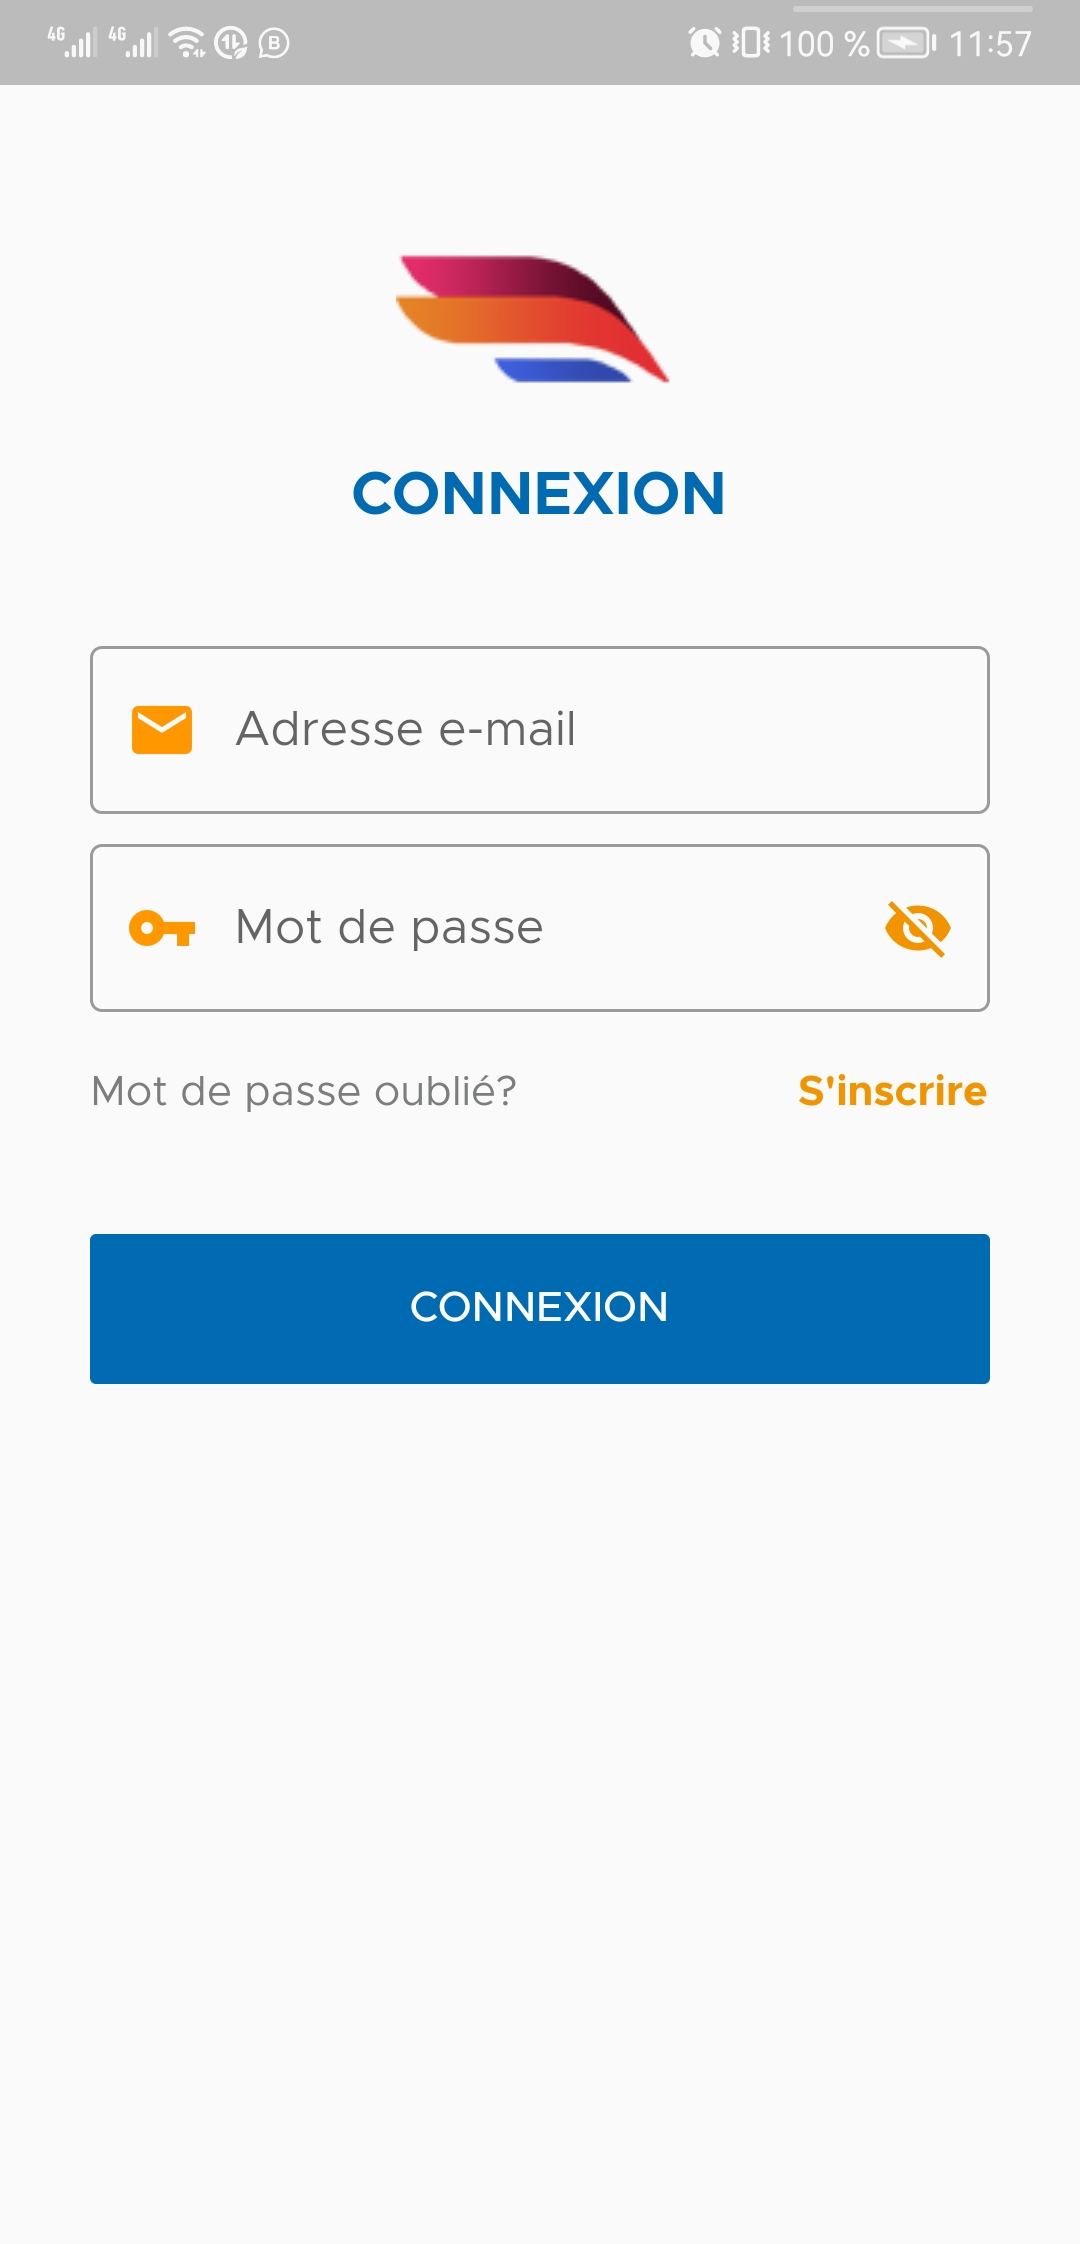
\includegraphics[width=5cm]{./Template LaTeX/Images/3.jpg} }}%
				\caption{Interface d'authentification}%
				\label{fig:example}%
			\end{figure}
		\newpage
		La demande d’identification du client est traitée pour vérifier ses paramètres dans la base de
		données. L’absence de l’utilisateur dans la base de données ou une erreur de saisie des
		informations entraine une alerte d’erreur d’authentification.\newline
		%%%%%%%%%%%%%%%%%%%%%%%%%% Inscruire %%%%%%%%%%%%%%%%%%%%%%5
		\item \textbf{L’interface d’inscription :}
		Avant de pouvoir s’authentifier, l’utilisateur doit
		impérativement s’enregistrer au préalable dans la base de données. La figure suivante
		représente l’interface de création de compte pour un client.Toutes les informations personnelles sont extraites partir de scan de code MRZ.
		\begin{figure}[!ht]
			\centering
			\begin{subfigure}{0.3\textwidth}
				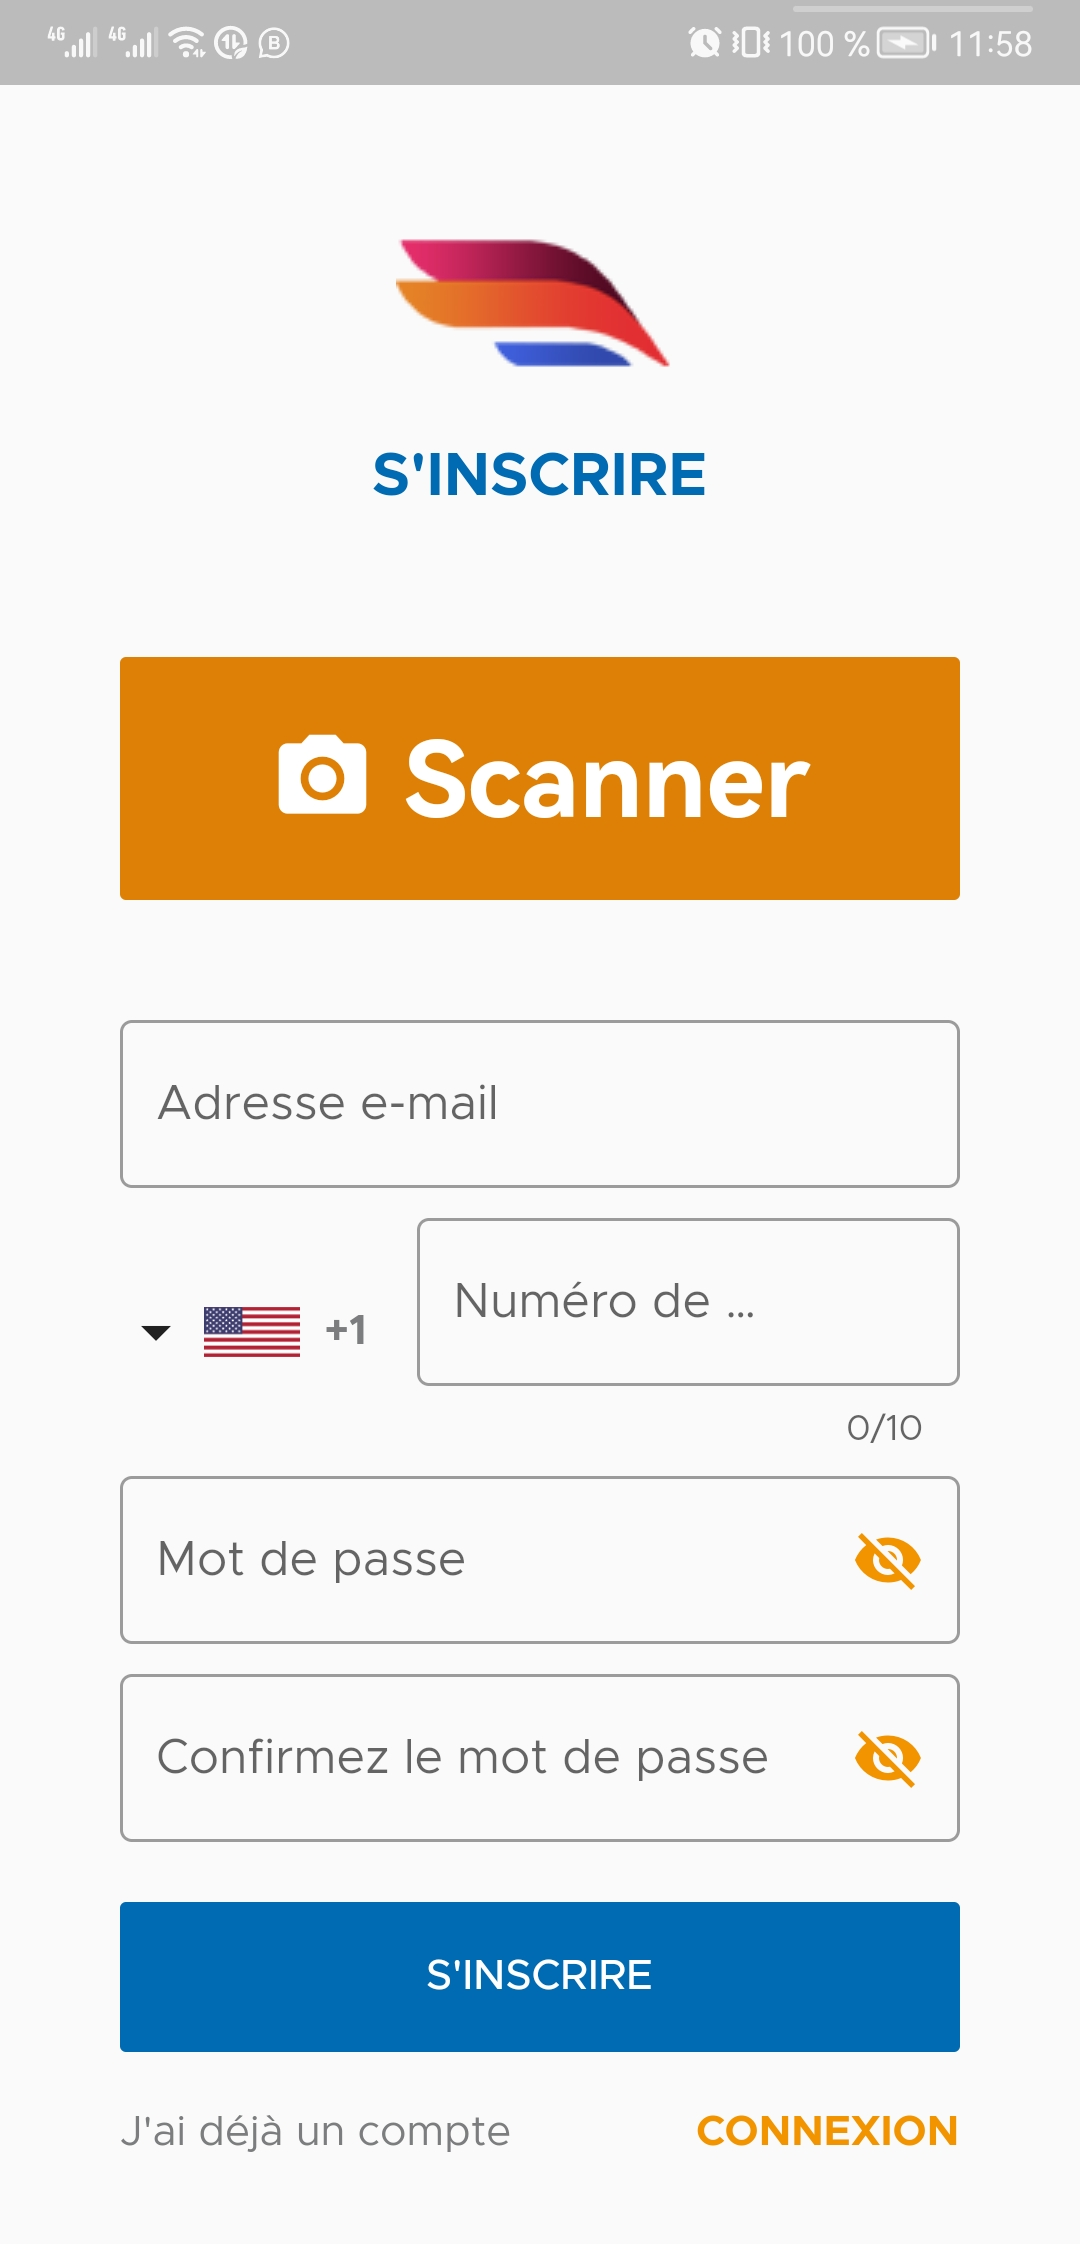
\includegraphics[width=\hsize, valign=m ]{./Template LaTeX/Images/4.jpg}
				\caption{Interface d’inscription}
				\label{fig.SICAPI}
			\end{subfigure}
			\qquad\tikz[baseline=-\baselineskip]\draw[ultra thick,->] (0,0) -- ++ (1,0);\qquad
			\begin{subfigure}{0.3\textwidth}
				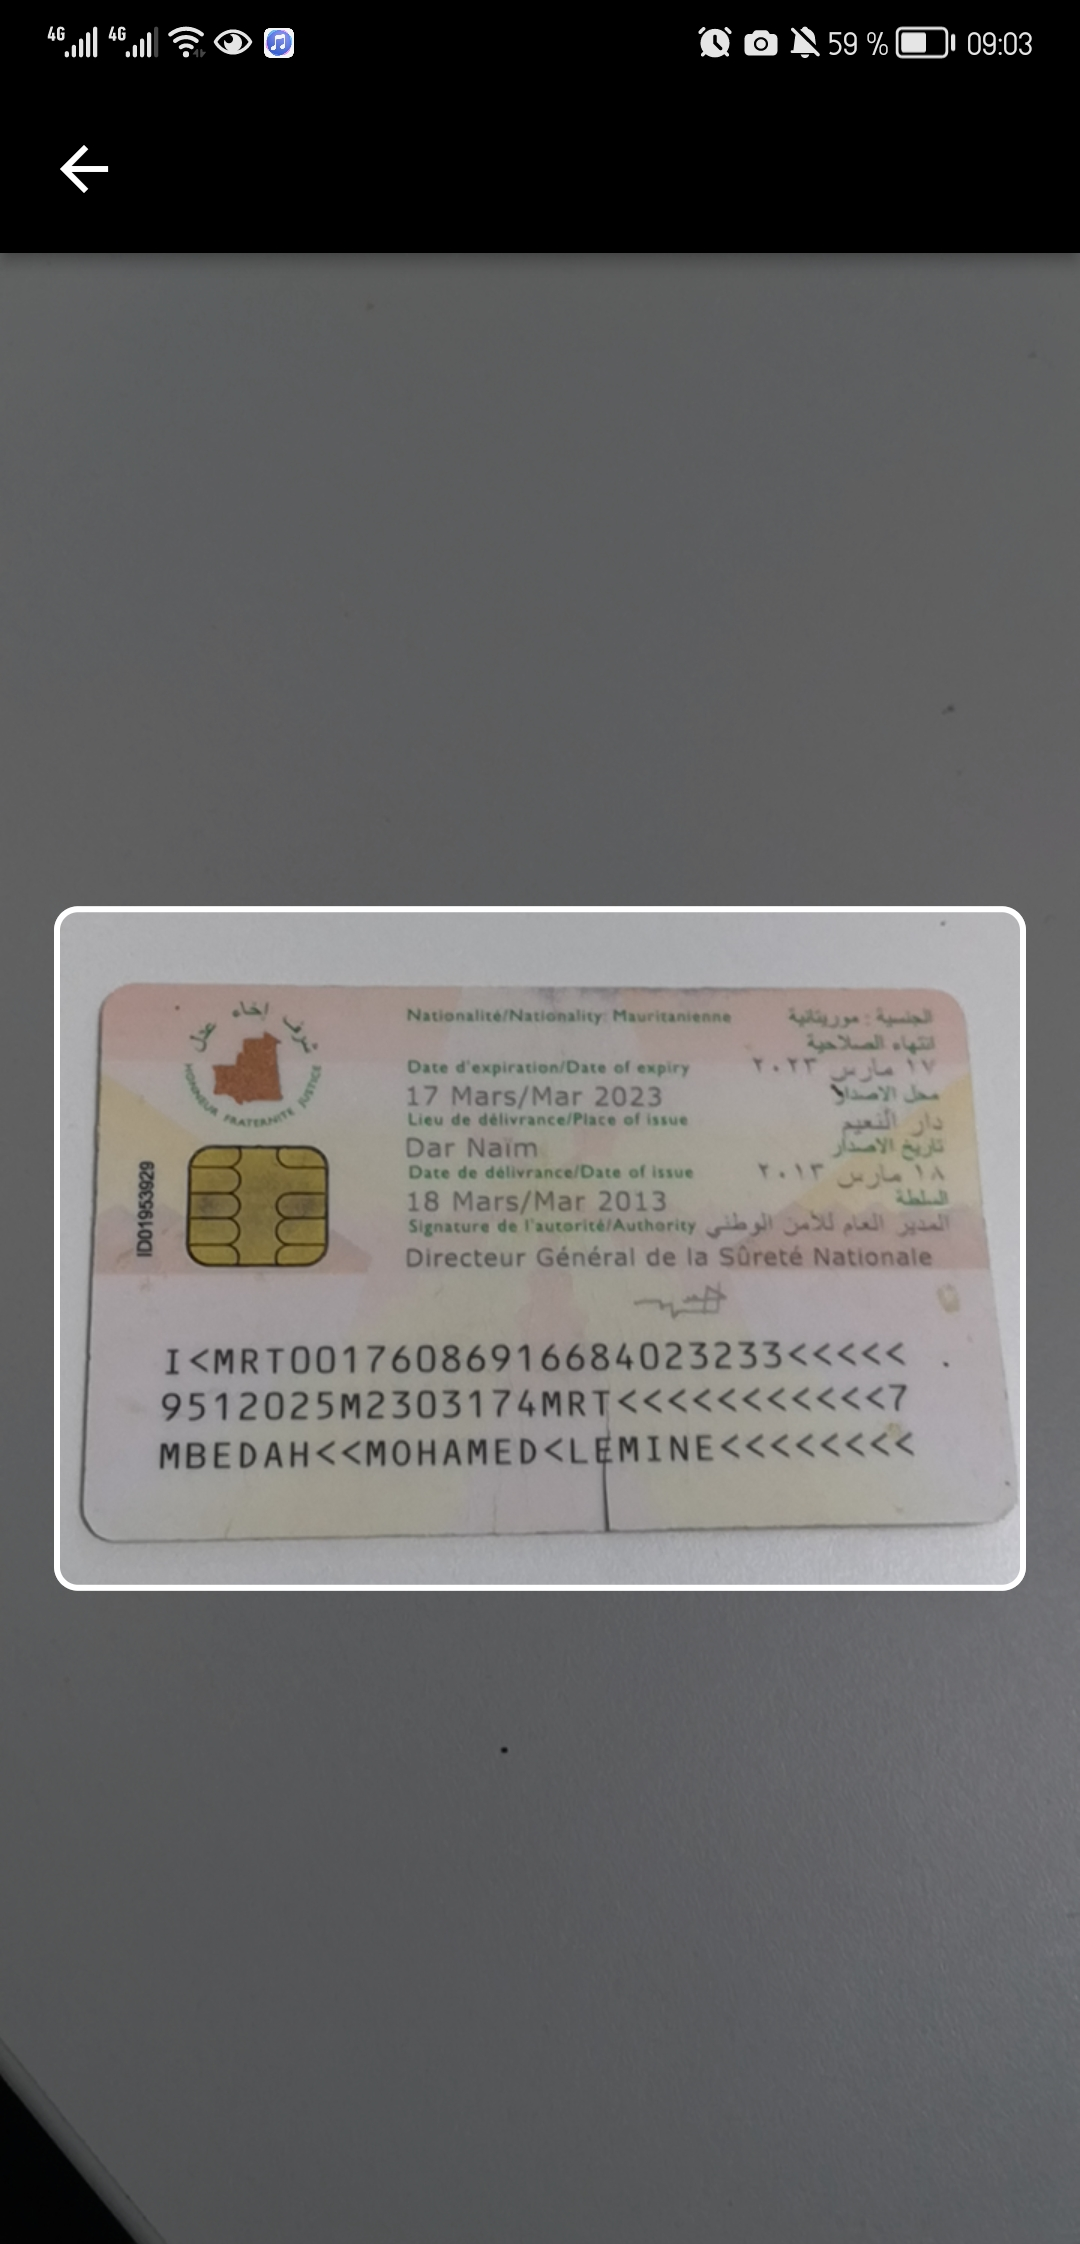
\includegraphics[width=\hsize, valign=m]{./Template LaTeX/Images/23.jpg}
				\caption{Scanner le code MRZ}
				\label{fig.painel_sicapi}
			\end{subfigure}
	
		\begin{subfigure}{0.3\textwidth}
			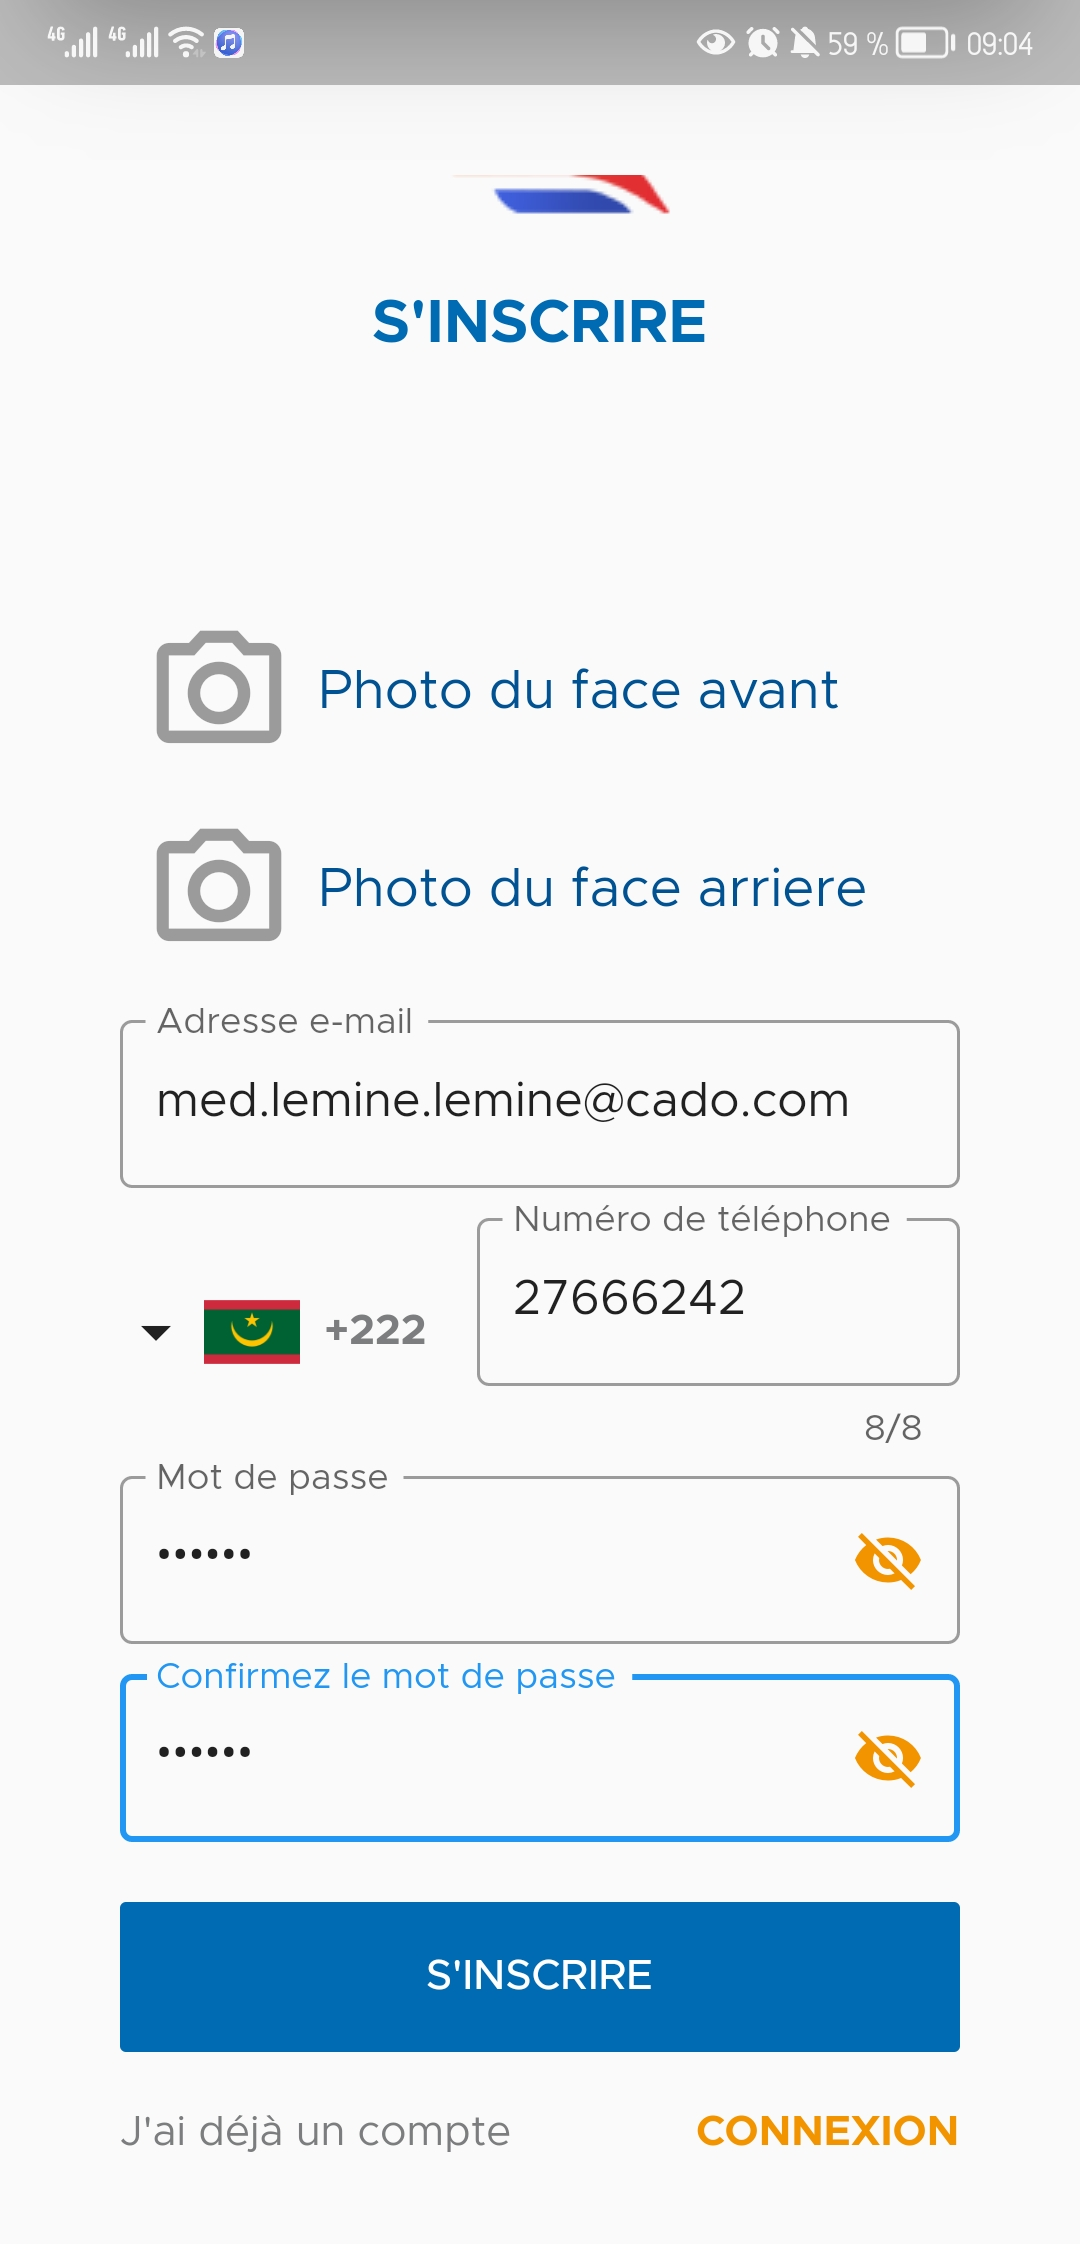
\includegraphics[width=\hsize, valign=m]{./Template LaTeX/Images/24.jpg}
			\caption{Saisir le rest des données}
			\label{fig.painel_sicapi}
		\end{subfigure}
			\caption{Interface d’inscription}
			\label{fig.sicapi}
		\end{figure}
	
	%%%%%%%%%%%%%%%%%%%%%%%%%%%%%5 Home
	
	%%%%%%%%%%%%%%%%%%%%%%%%%%%%%%%%%%%%
	\newpage
	\item \textbf{Processus de la transaction
		:} La figure suivante montre les processus de la transaction depuis la sélection de montant jusqu'à la validation (une notification de succès va Apparence si le traitement se fait avec succès)
\begin{comment}
	content...

\begin{figure}[!ht]
	\centering
	\begin{subfigure}{0.3\textwidth}
		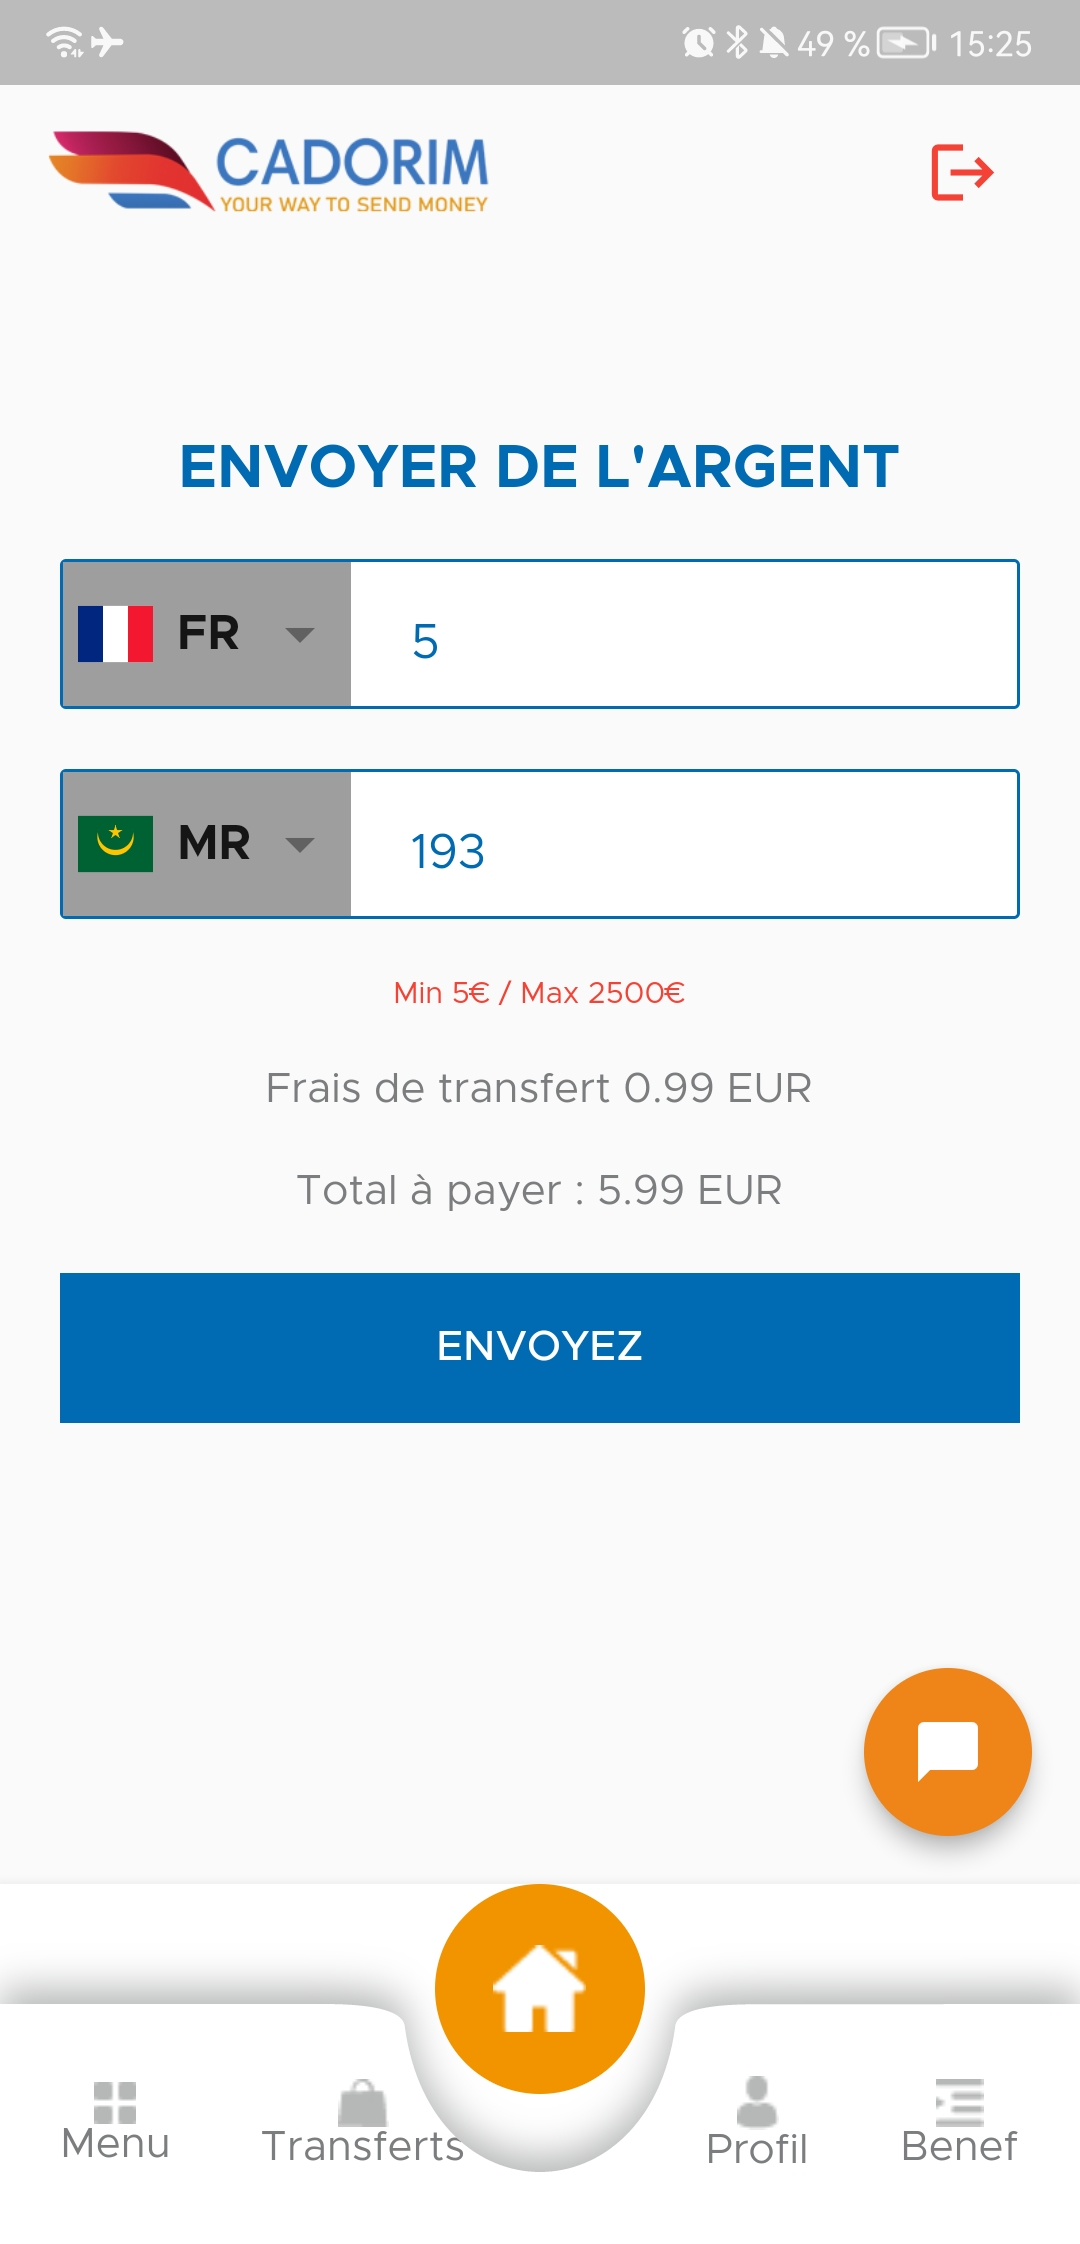
\includegraphics[width=\hsize, valign=m ]{./Template LaTeX/Images/5.jpg}
		\caption{Interfaces d'accueil}
		\label{fig.SICAPI}
	\end{subfigure}
	\qquad\tikz[baseline=-\baselineskip]\draw[ultra thick,->] (0,0) -- ++ (1,0);\qquad
	\begin{subfigure}{0.3\textwidth}
		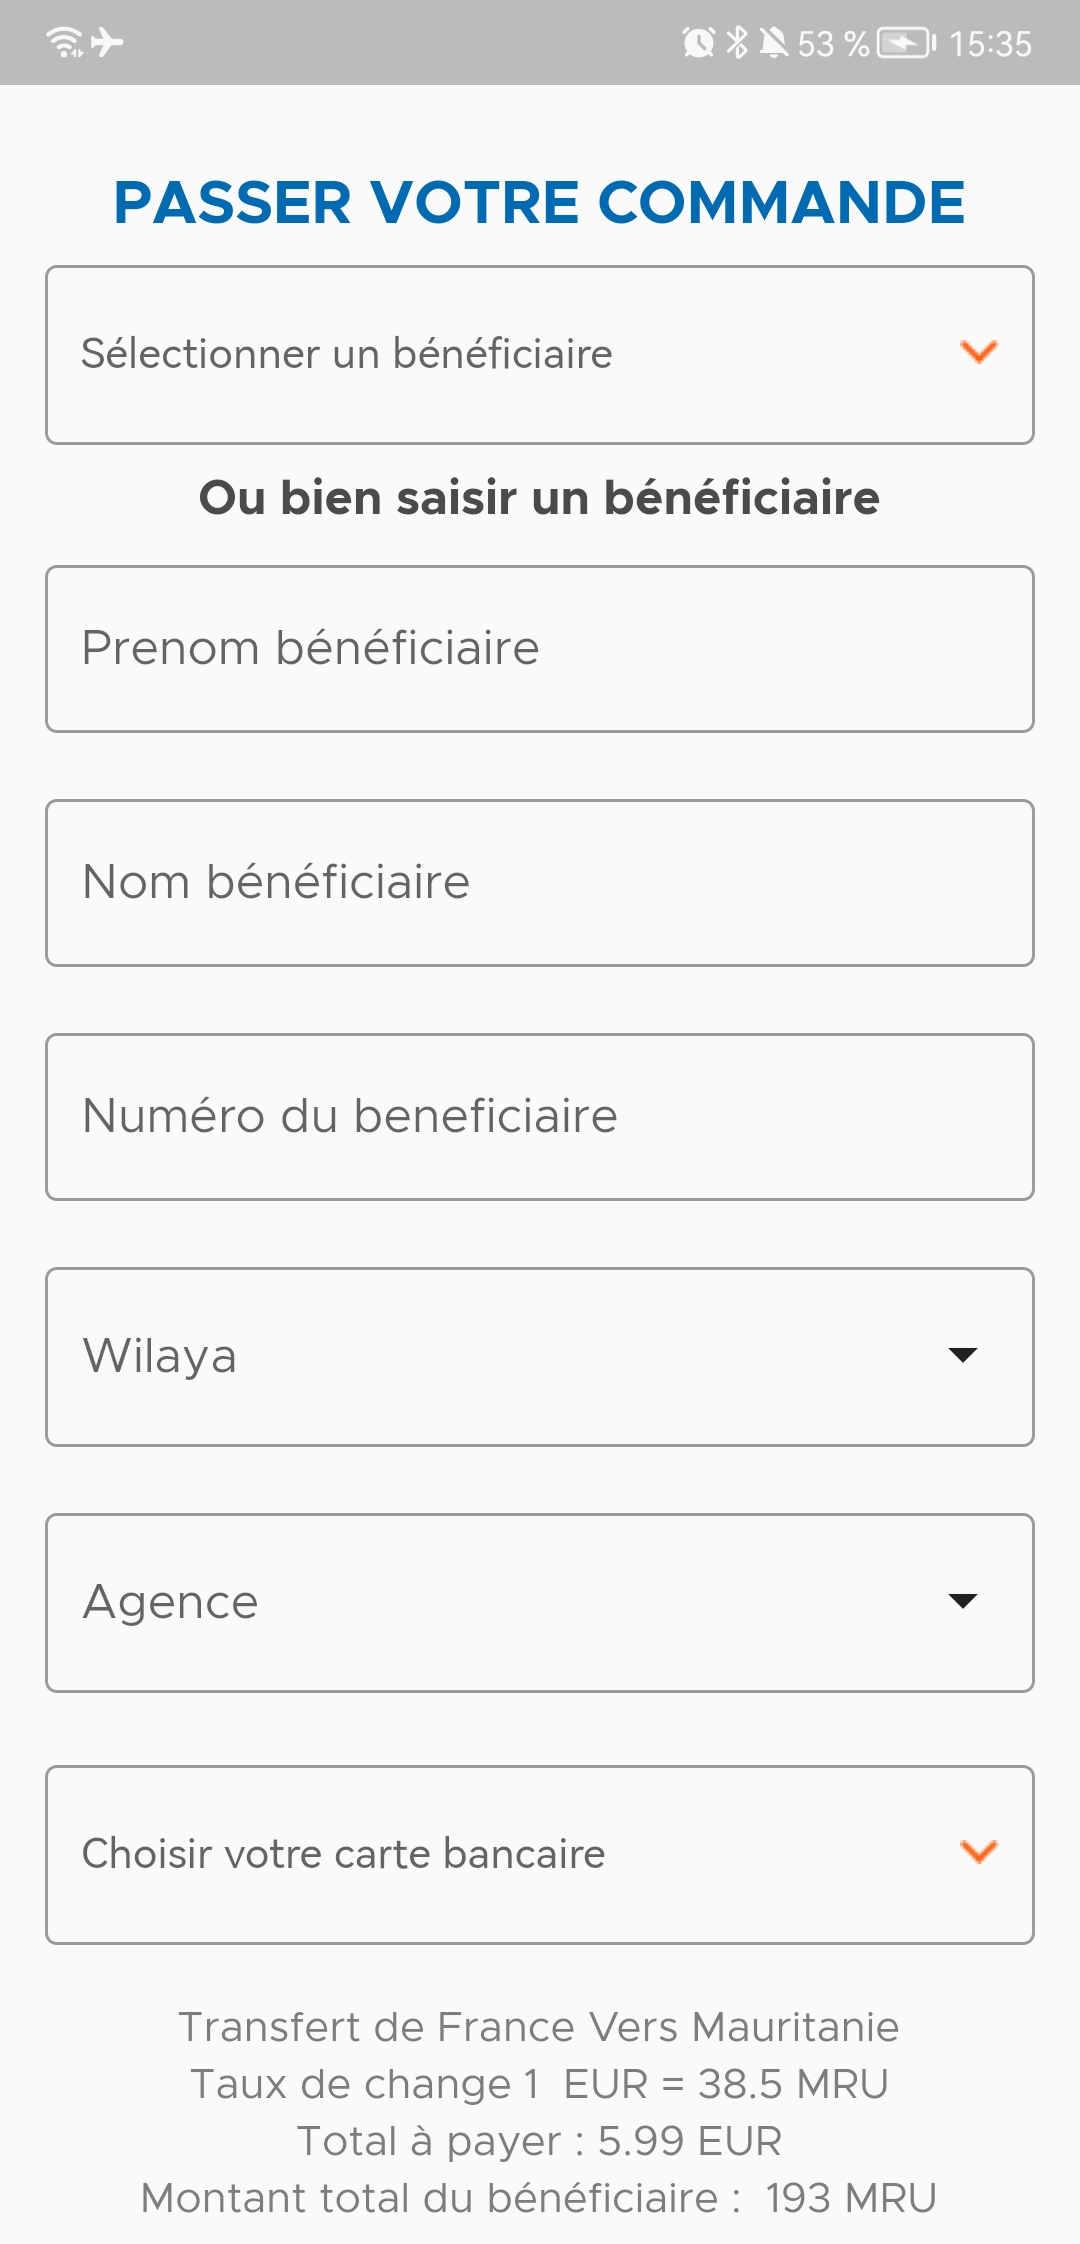
\includegraphics[width=\hsize, valign=m]{./Template LaTeX/Images/11.jpg}
		\caption{Interface de transfert}
		\label{fig.painel_sicapi}
	\end{subfigure}
%%%%%%%%%%%%%%%%%%%%%%%%%%%%%
\begin{subfigure}{0.3\textwidth}
	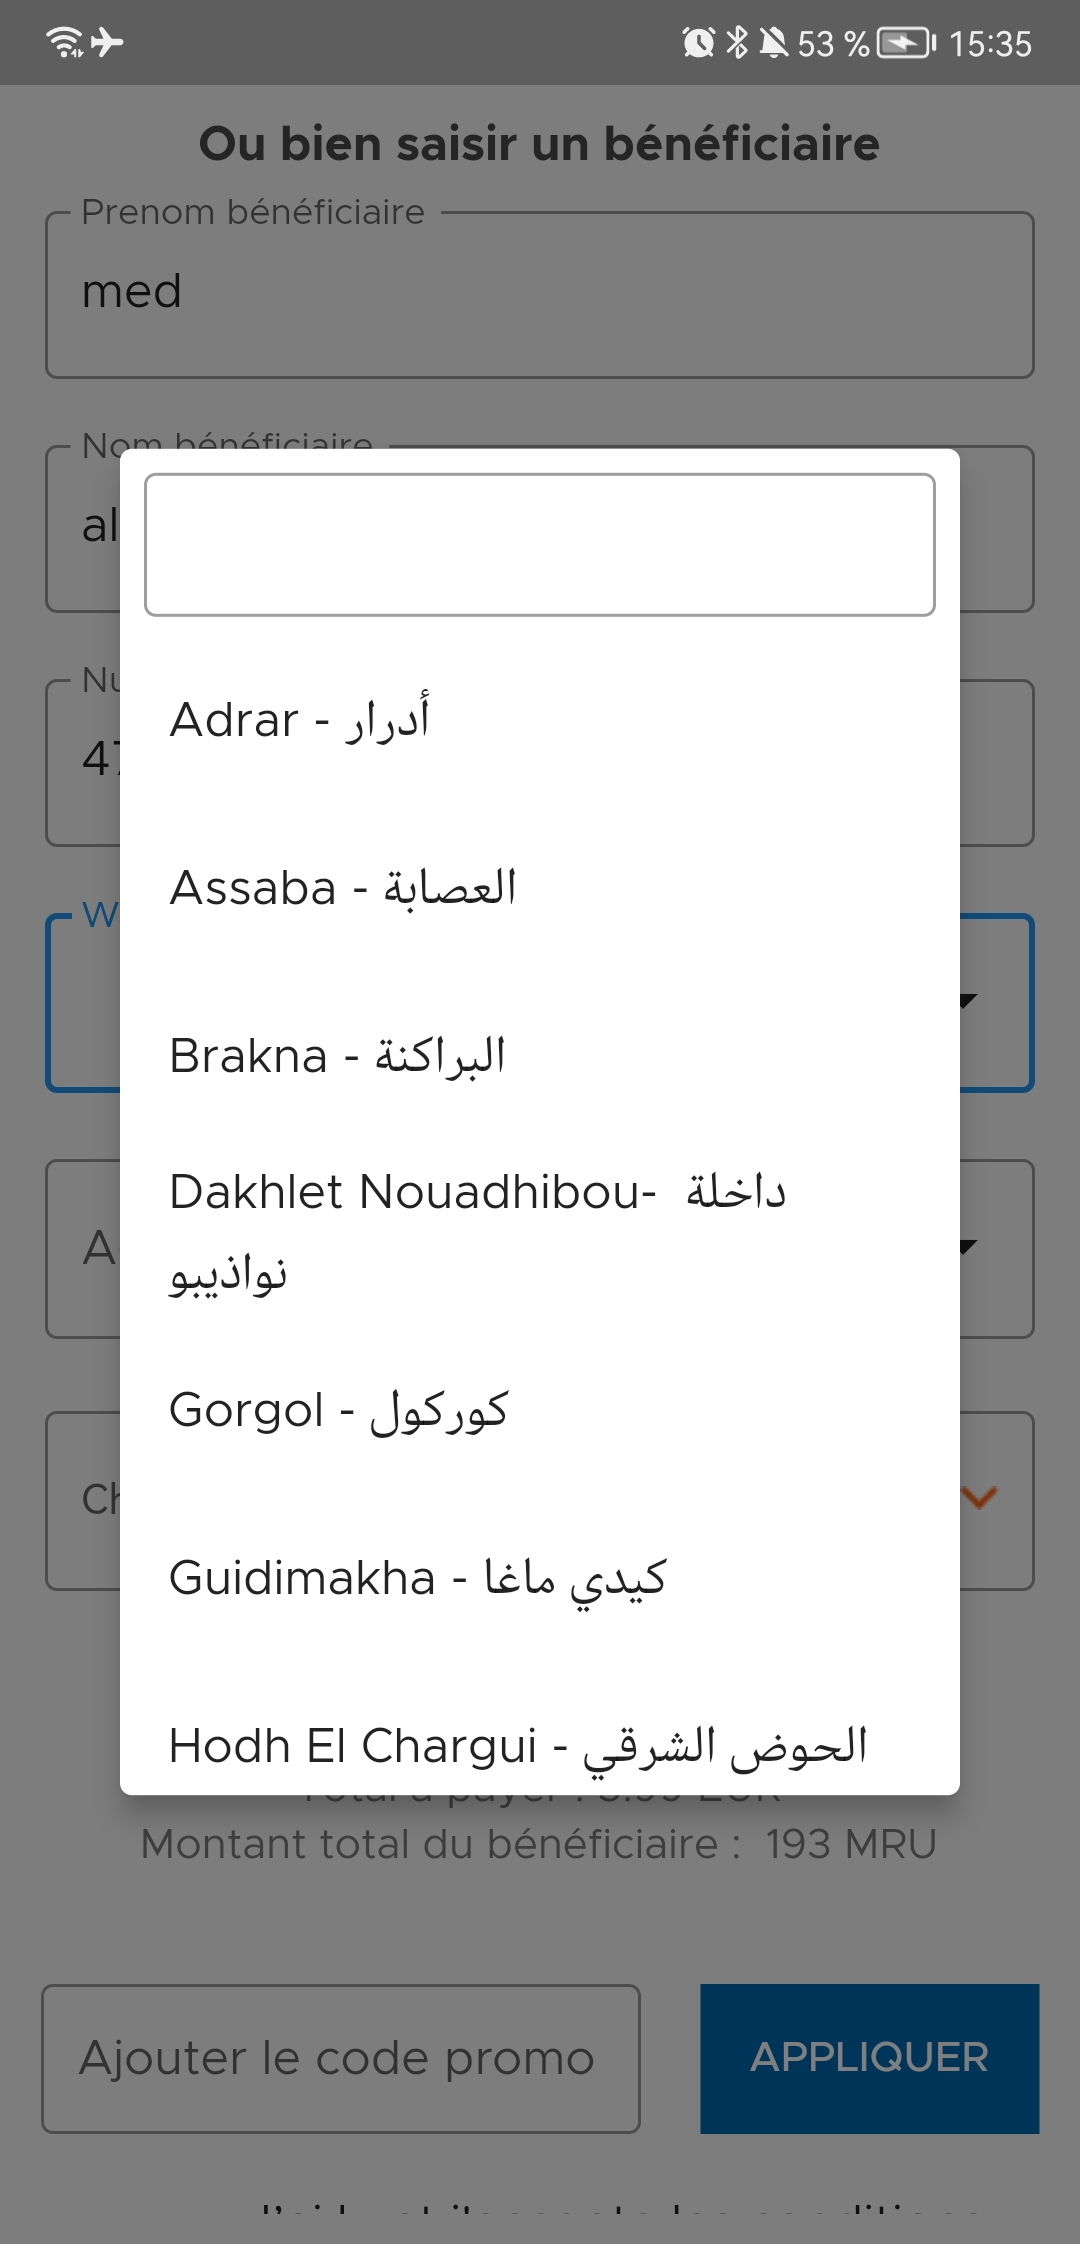
\includegraphics[width=\hsize, valign=m ]{./Template LaTeX/Images/12.jpg}
	\caption{Choix de wilaya}
	\label{fig.SICAPI}
\end{subfigure}
\qquad\tikz[baseline=-\baselineskip]\draw[ultra thick,->] (0,0) -- ++ (1,0);\qquad
\begin{subfigure}{0.3\textwidth}
	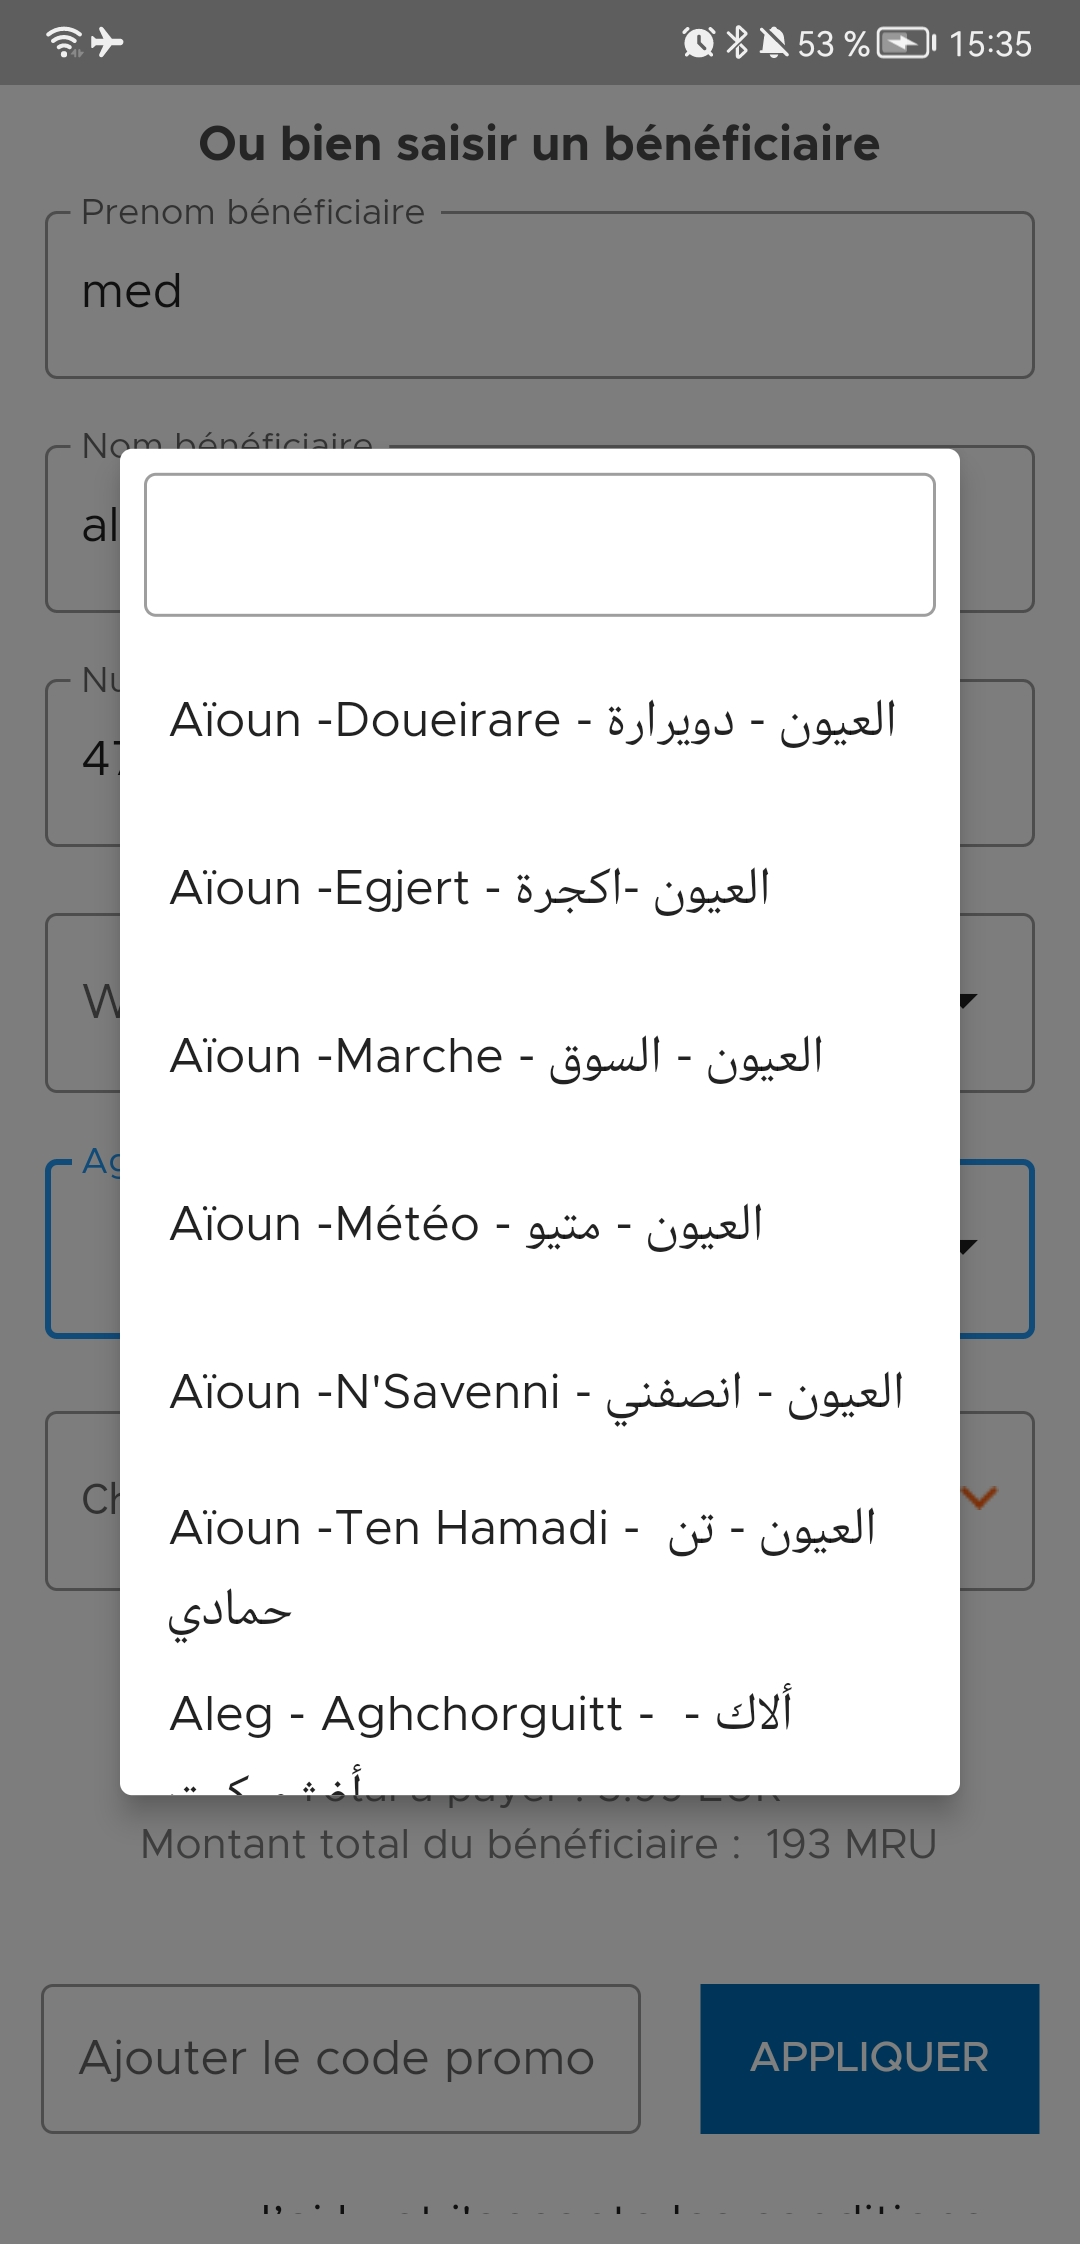
\includegraphics[width=\hsize, valign=m]{./Template LaTeX/Images/13.jpg}
	\caption{Choix d'agence}
	\label{fig.painel_sicapi}
\end{subfigure}
%%%%%%%%%%%%%%%%%%%%%%%%%%%%%%%%%%%%%%%%%%%%%%%%%%%%%%%%%%%

	\caption{Interfaces d'accueil}
	\label{fig.sicapi}
\end{figure}
\end{comment}
\begin{figure}
	\centering
	\begin{subfigure}[b]{0.3\textwidth}
		\centering
		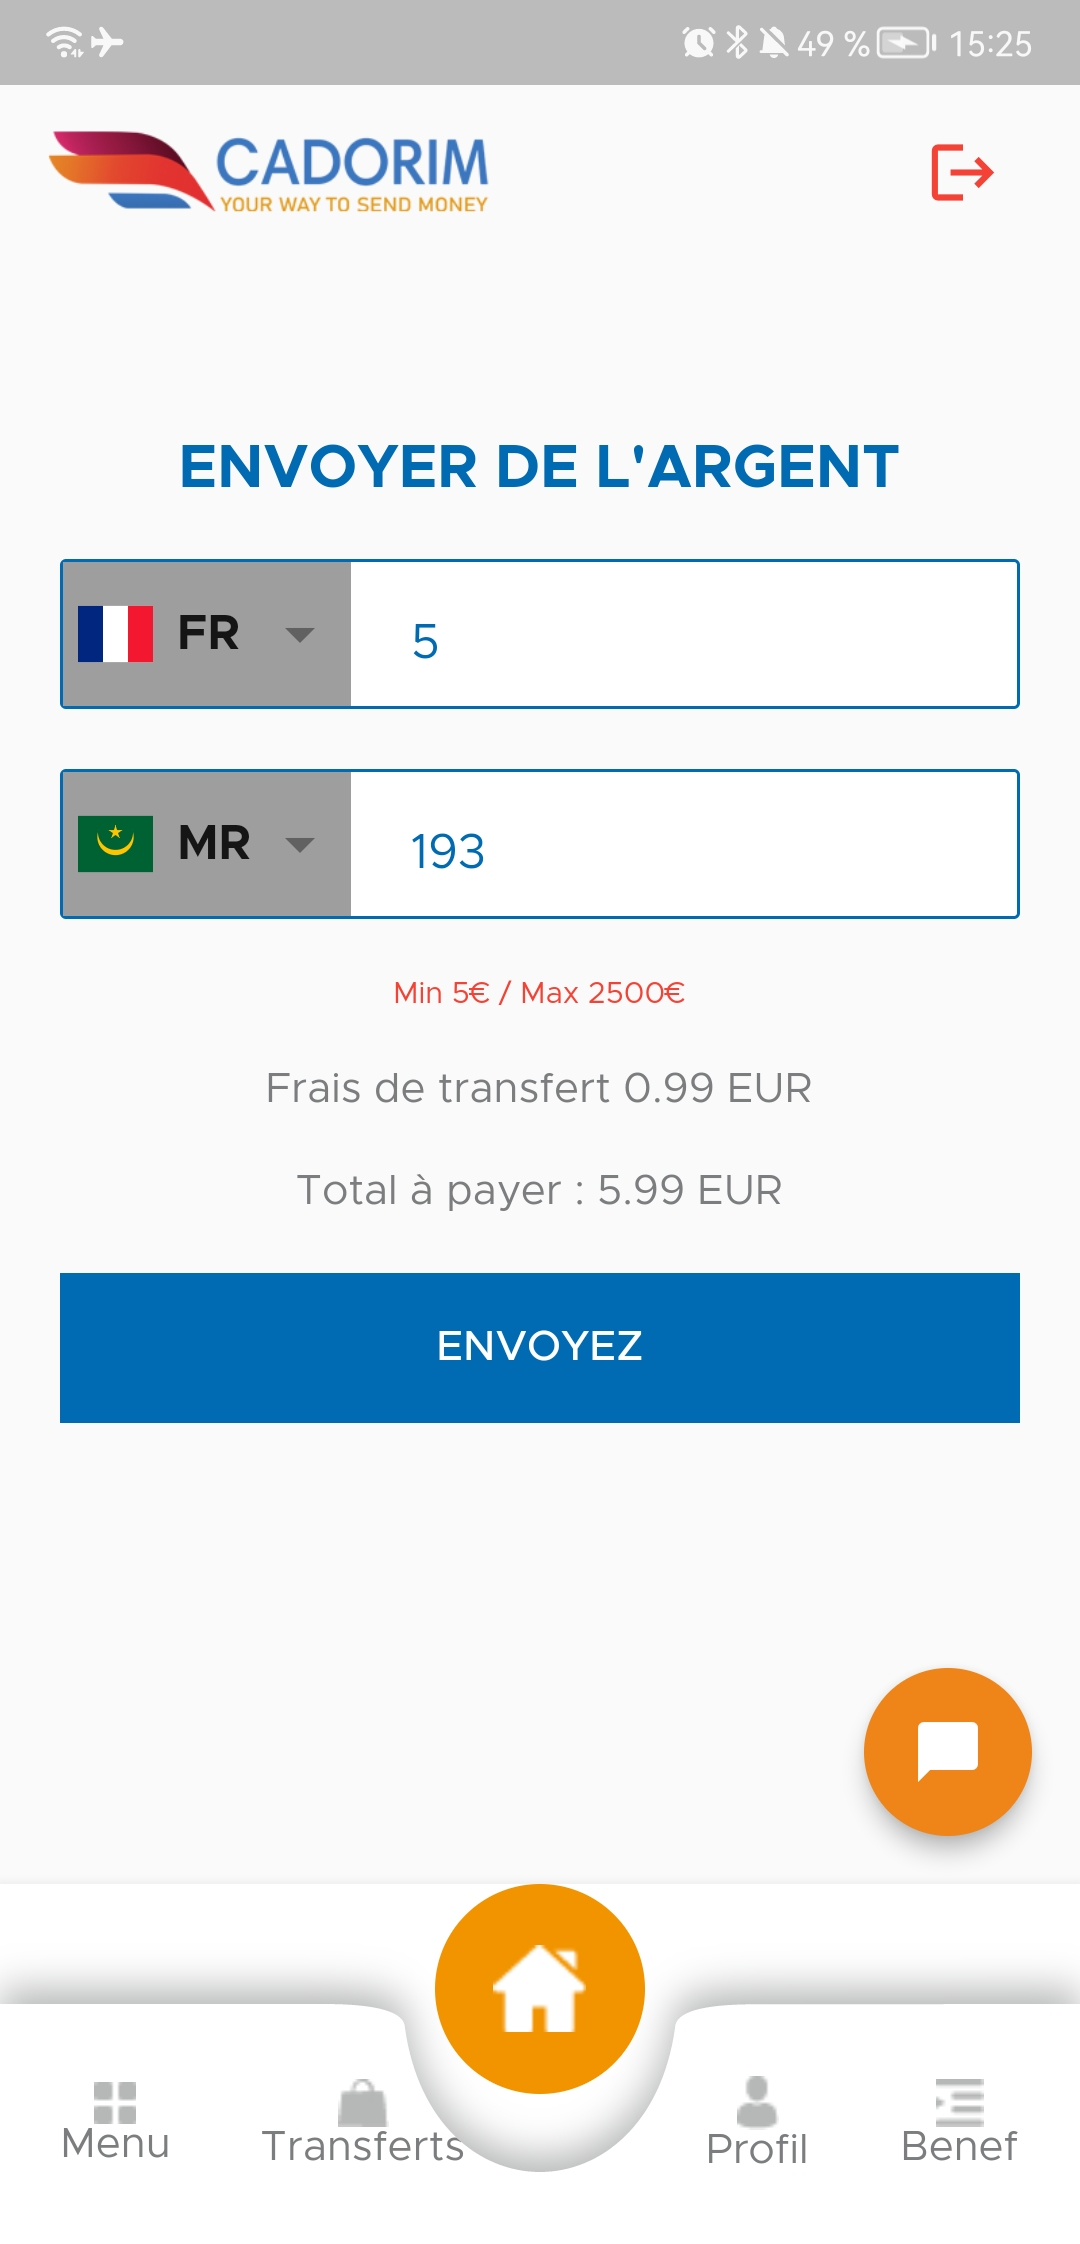
\includegraphics[width=\textwidth]{./Template LaTeX/Images/5.jpg}
		\caption{Interfaces d'accueil}
		\label{fig:y equals x}
	\end{subfigure}
	\hfill
	\begin{subfigure}[b]{0.3\textwidth}
		\centering
		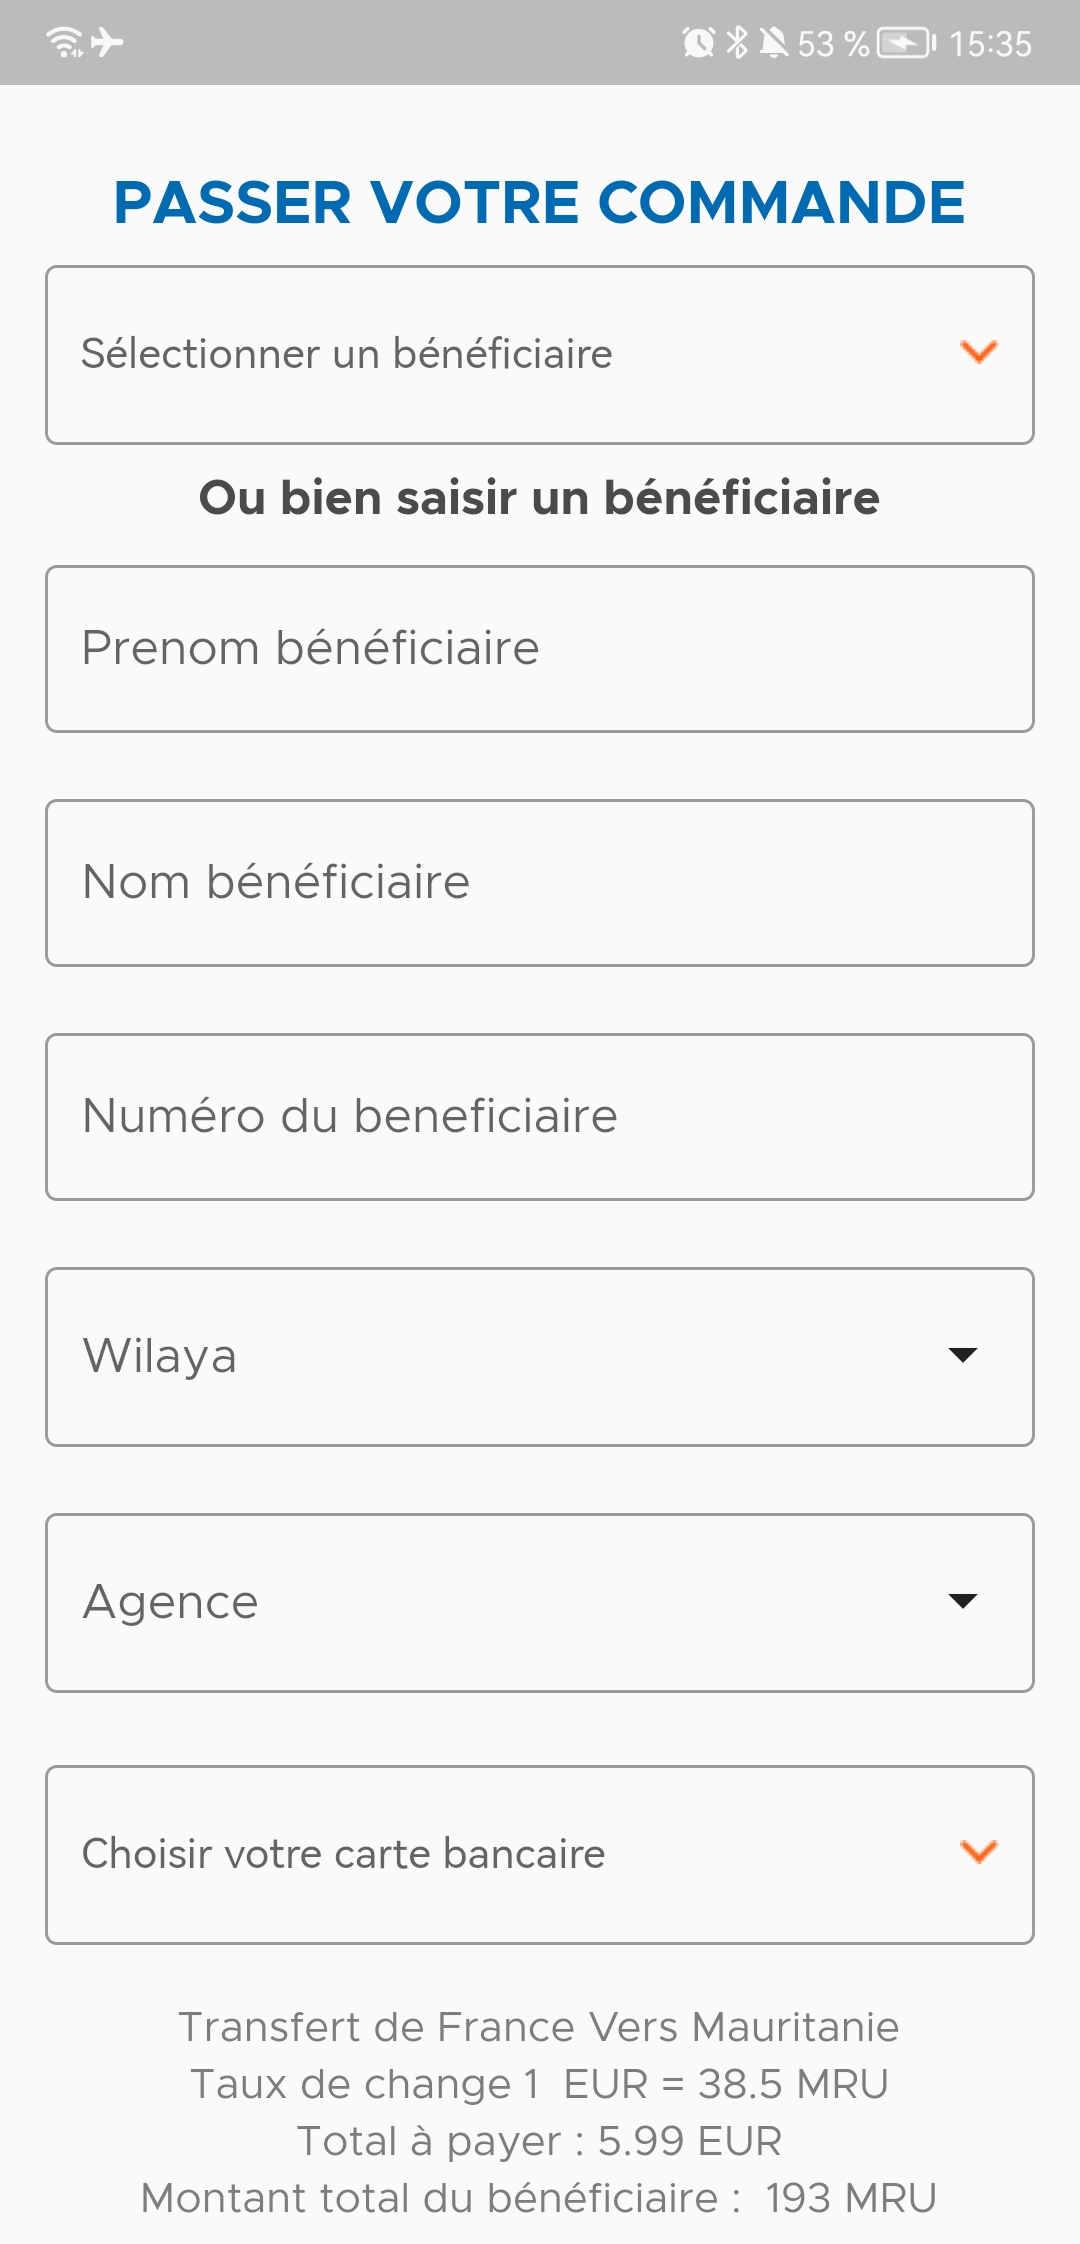
\includegraphics[width=\textwidth]{./Template LaTeX/Images/11.jpg}
		\caption{Interface de transfert}
		\label{fig:three sin x}
	\end{subfigure}
	\hfill
	\begin{subfigure}[b]{0.3\textwidth}
		\centering
		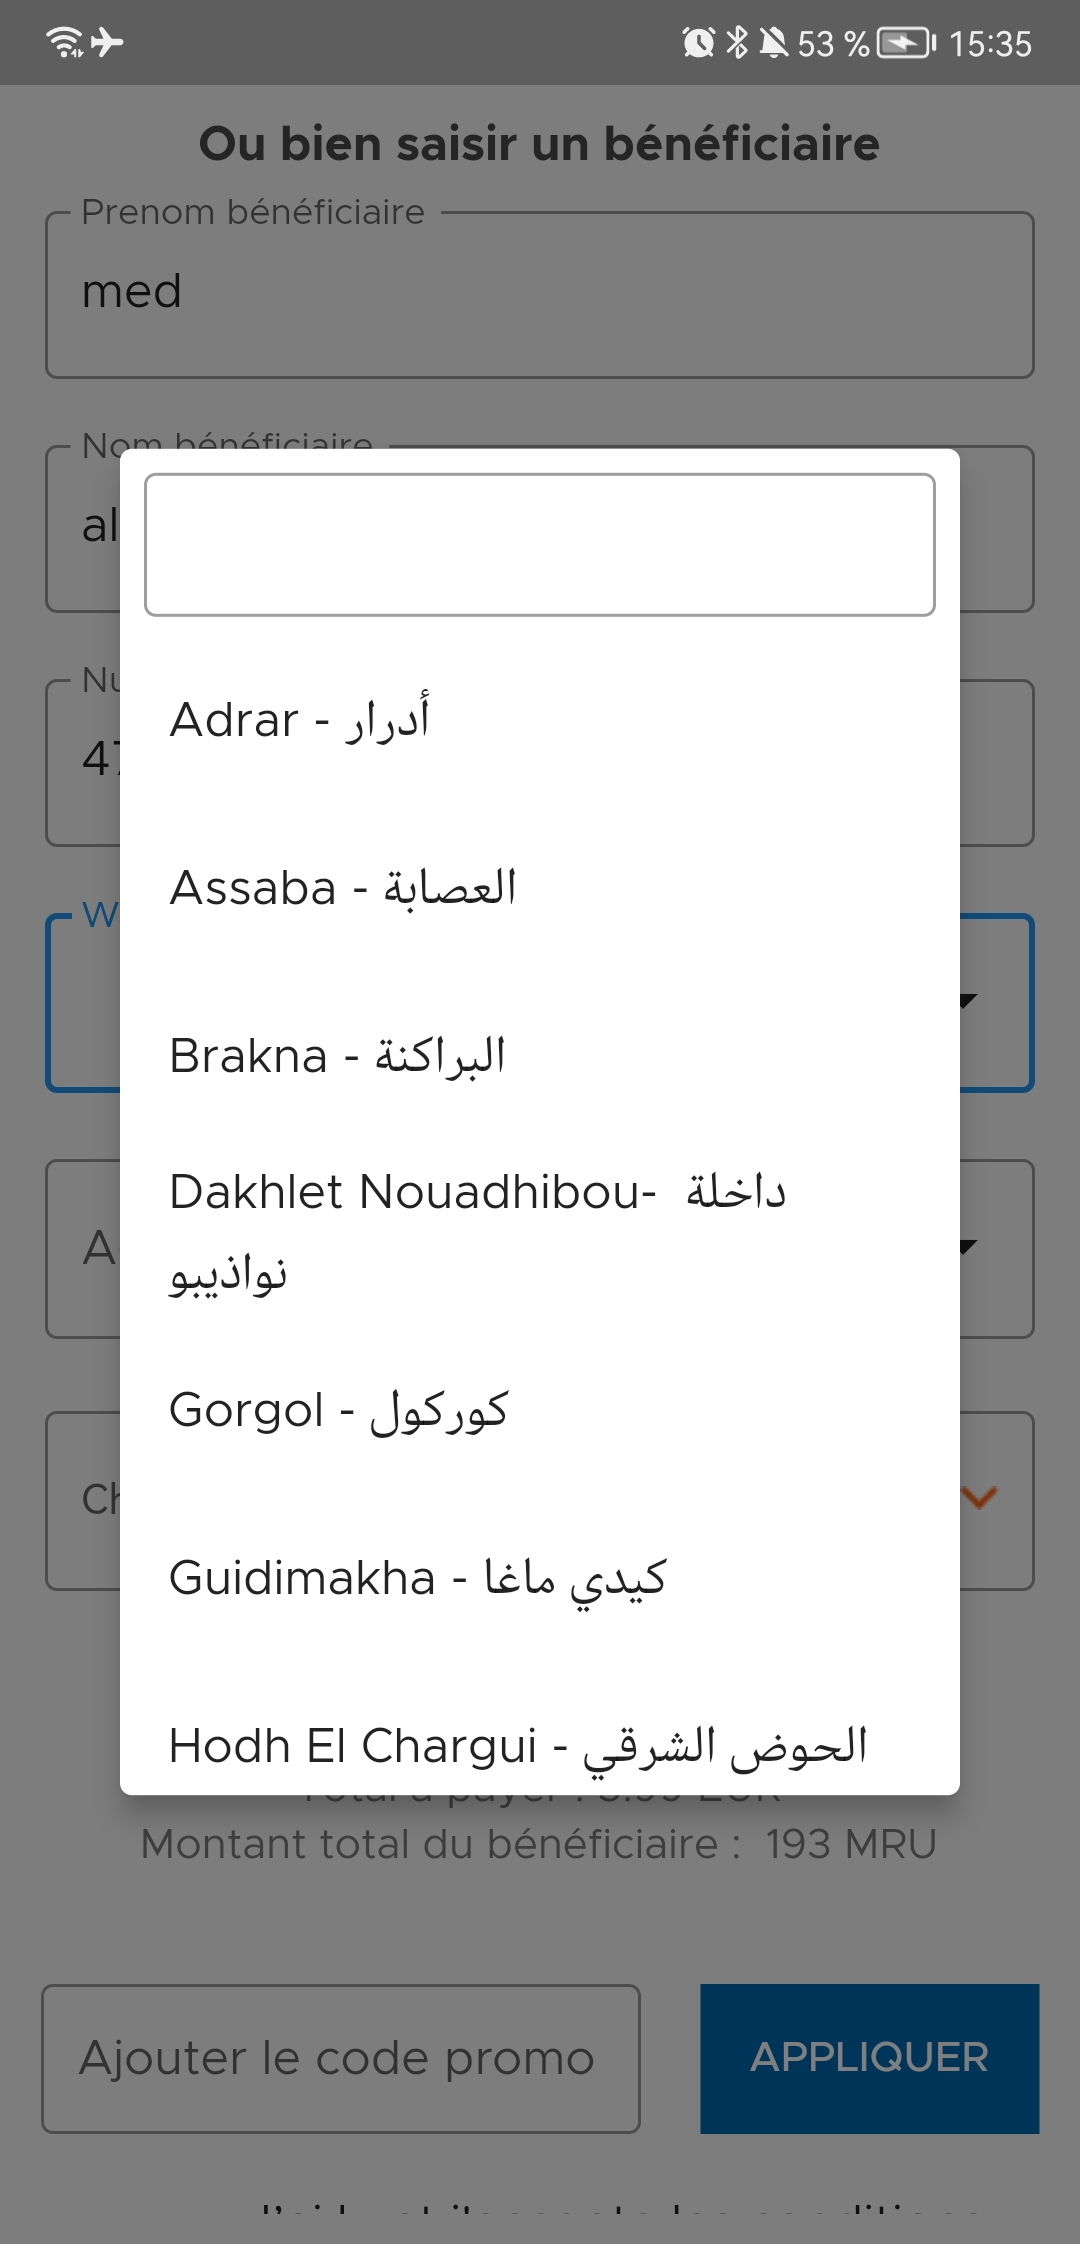
\includegraphics[width=\textwidth]{./Template LaTeX/Images/12.jpg}
		\caption{Choix de wilaya}
		\label{fig:five over x}
	\end{subfigure}
	\newline
		\centering
	\begin{subfigure}[b]{0.3\textwidth}
		\centering
		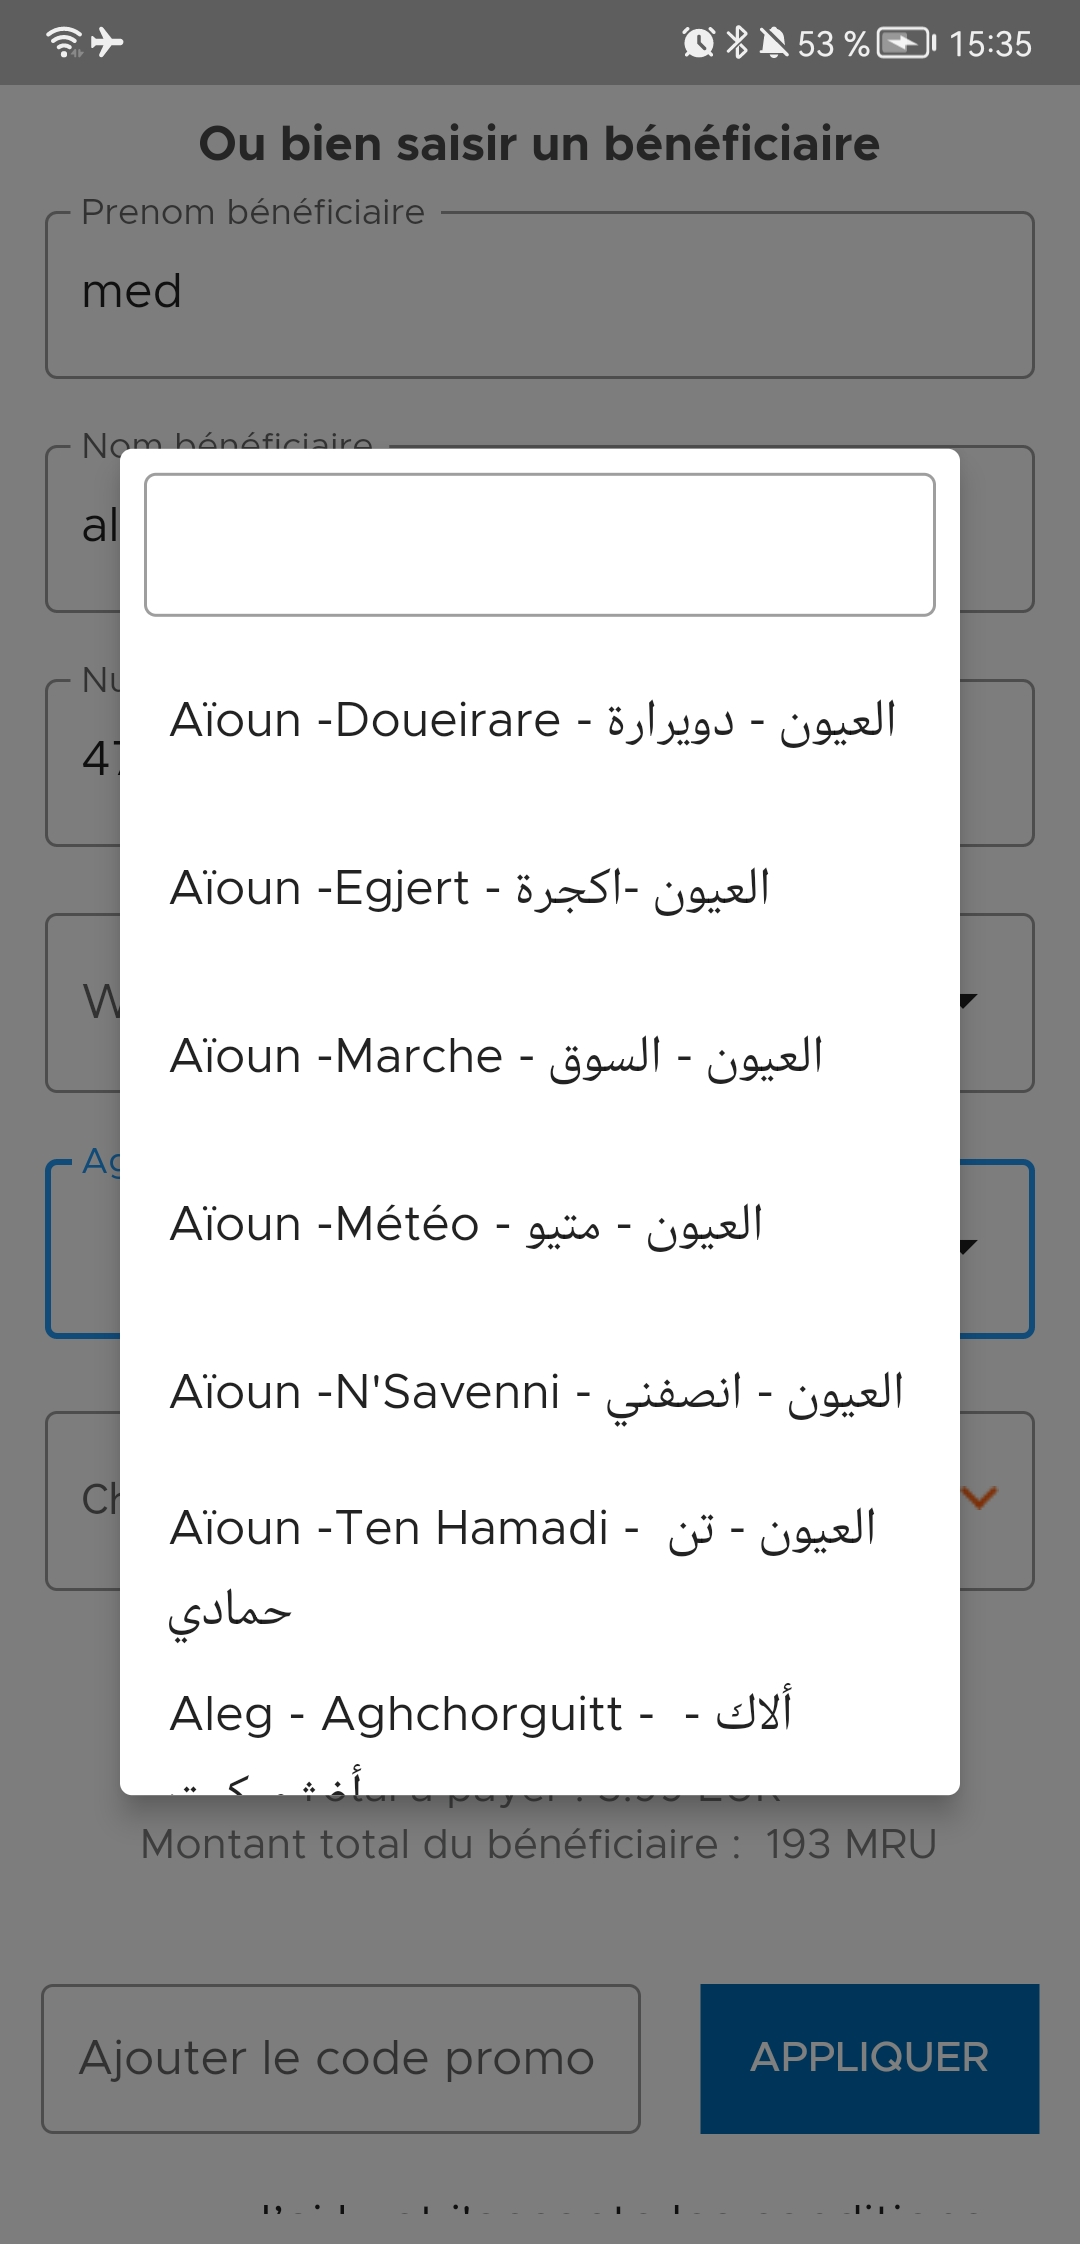
\includegraphics[width=\textwidth]{./Template LaTeX/Images/13.jpg}
		\caption{Choix d'agence}
		\label{fig:y equals x}
	\end{subfigure}
	\hfill
	\begin{subfigure}[b]{0.3\textwidth}
		\centering
		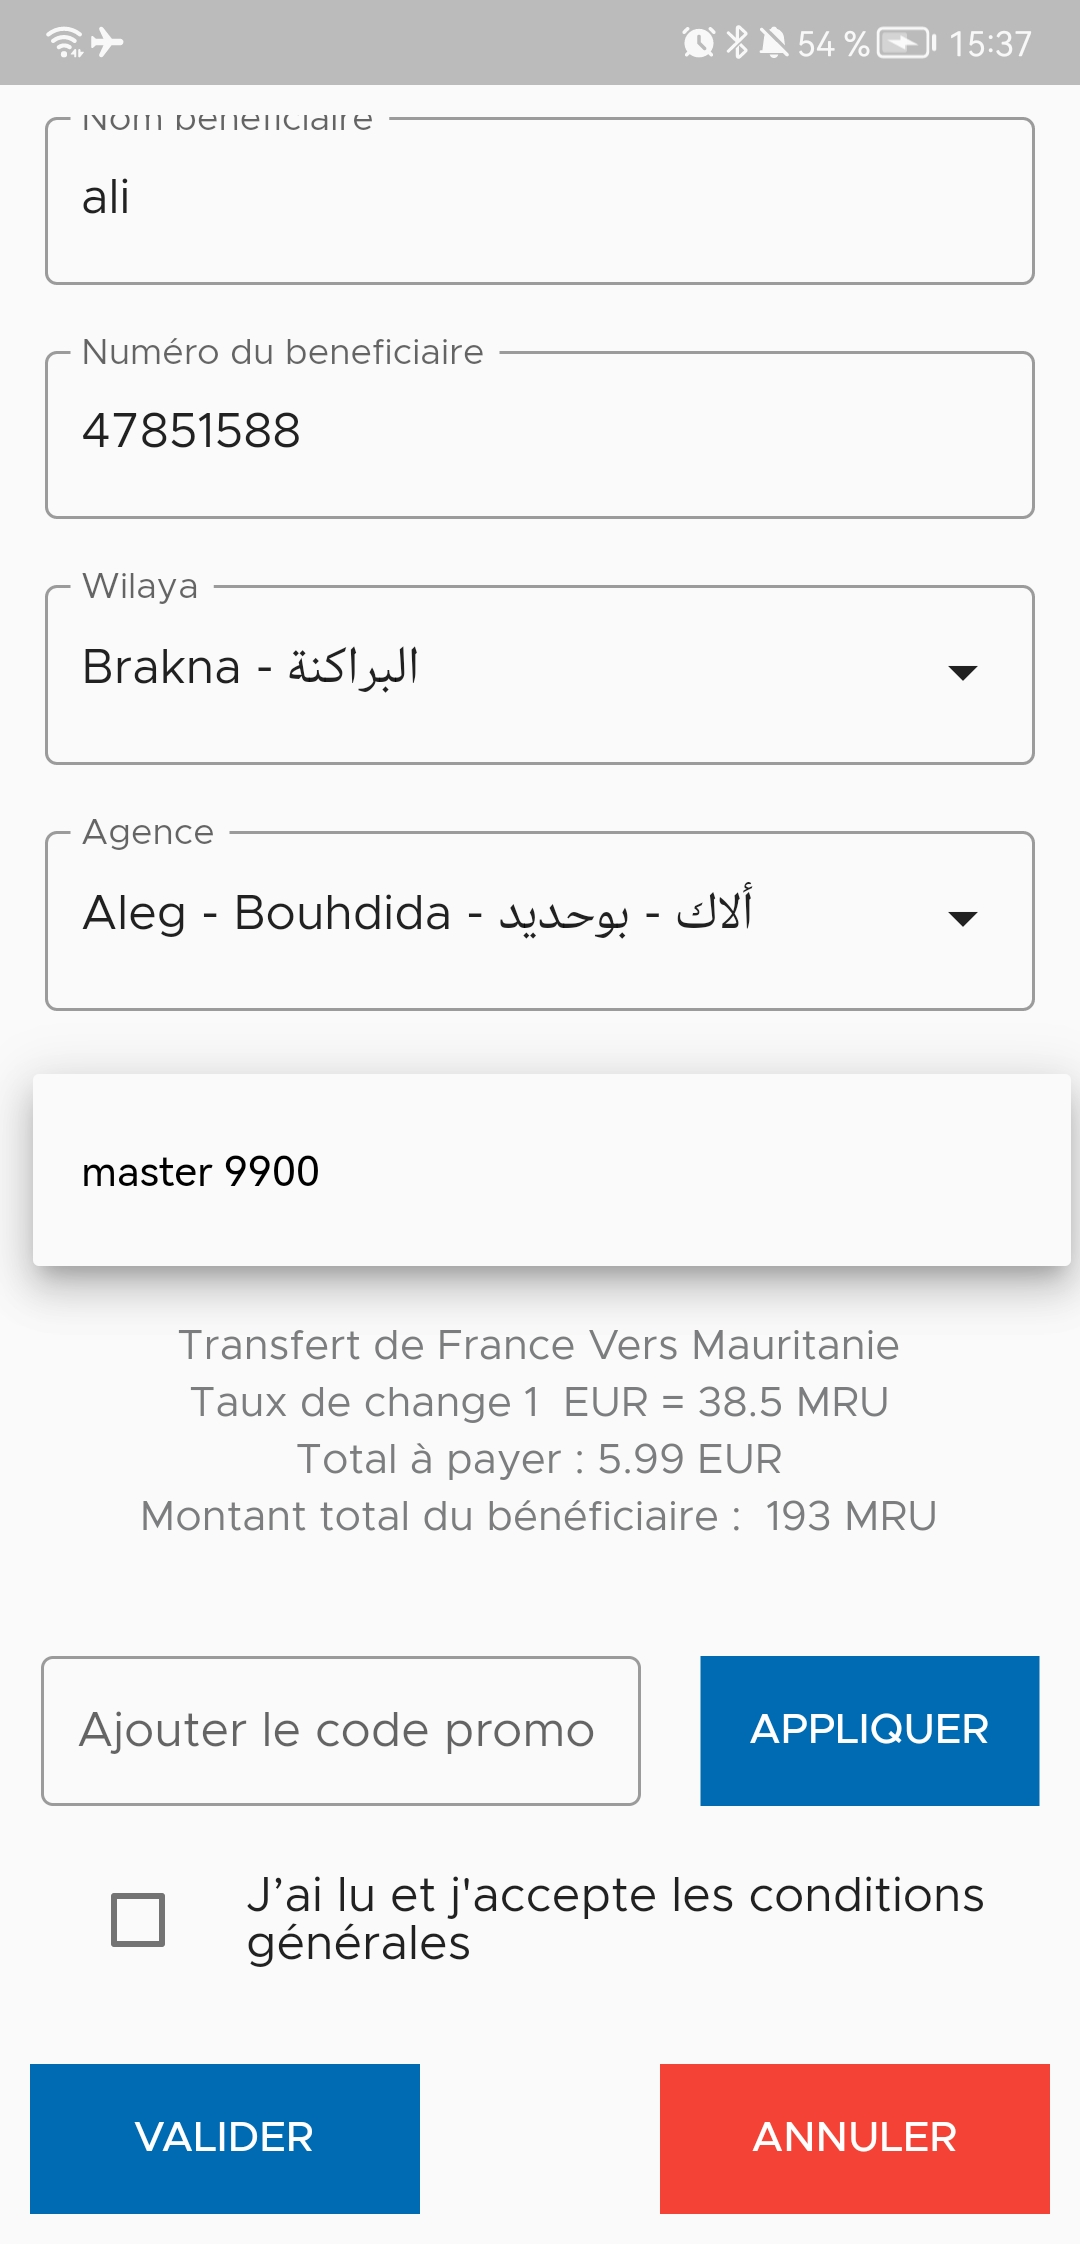
\includegraphics[width=\textwidth]{./Template LaTeX/Images/14.jpg}
		\caption{Choix de catre bancaire}
		\label{fig:three sin x}
	\end{subfigure}
	\hfill
	\begin{subfigure}[b]{0.3\textwidth}
		\centering
		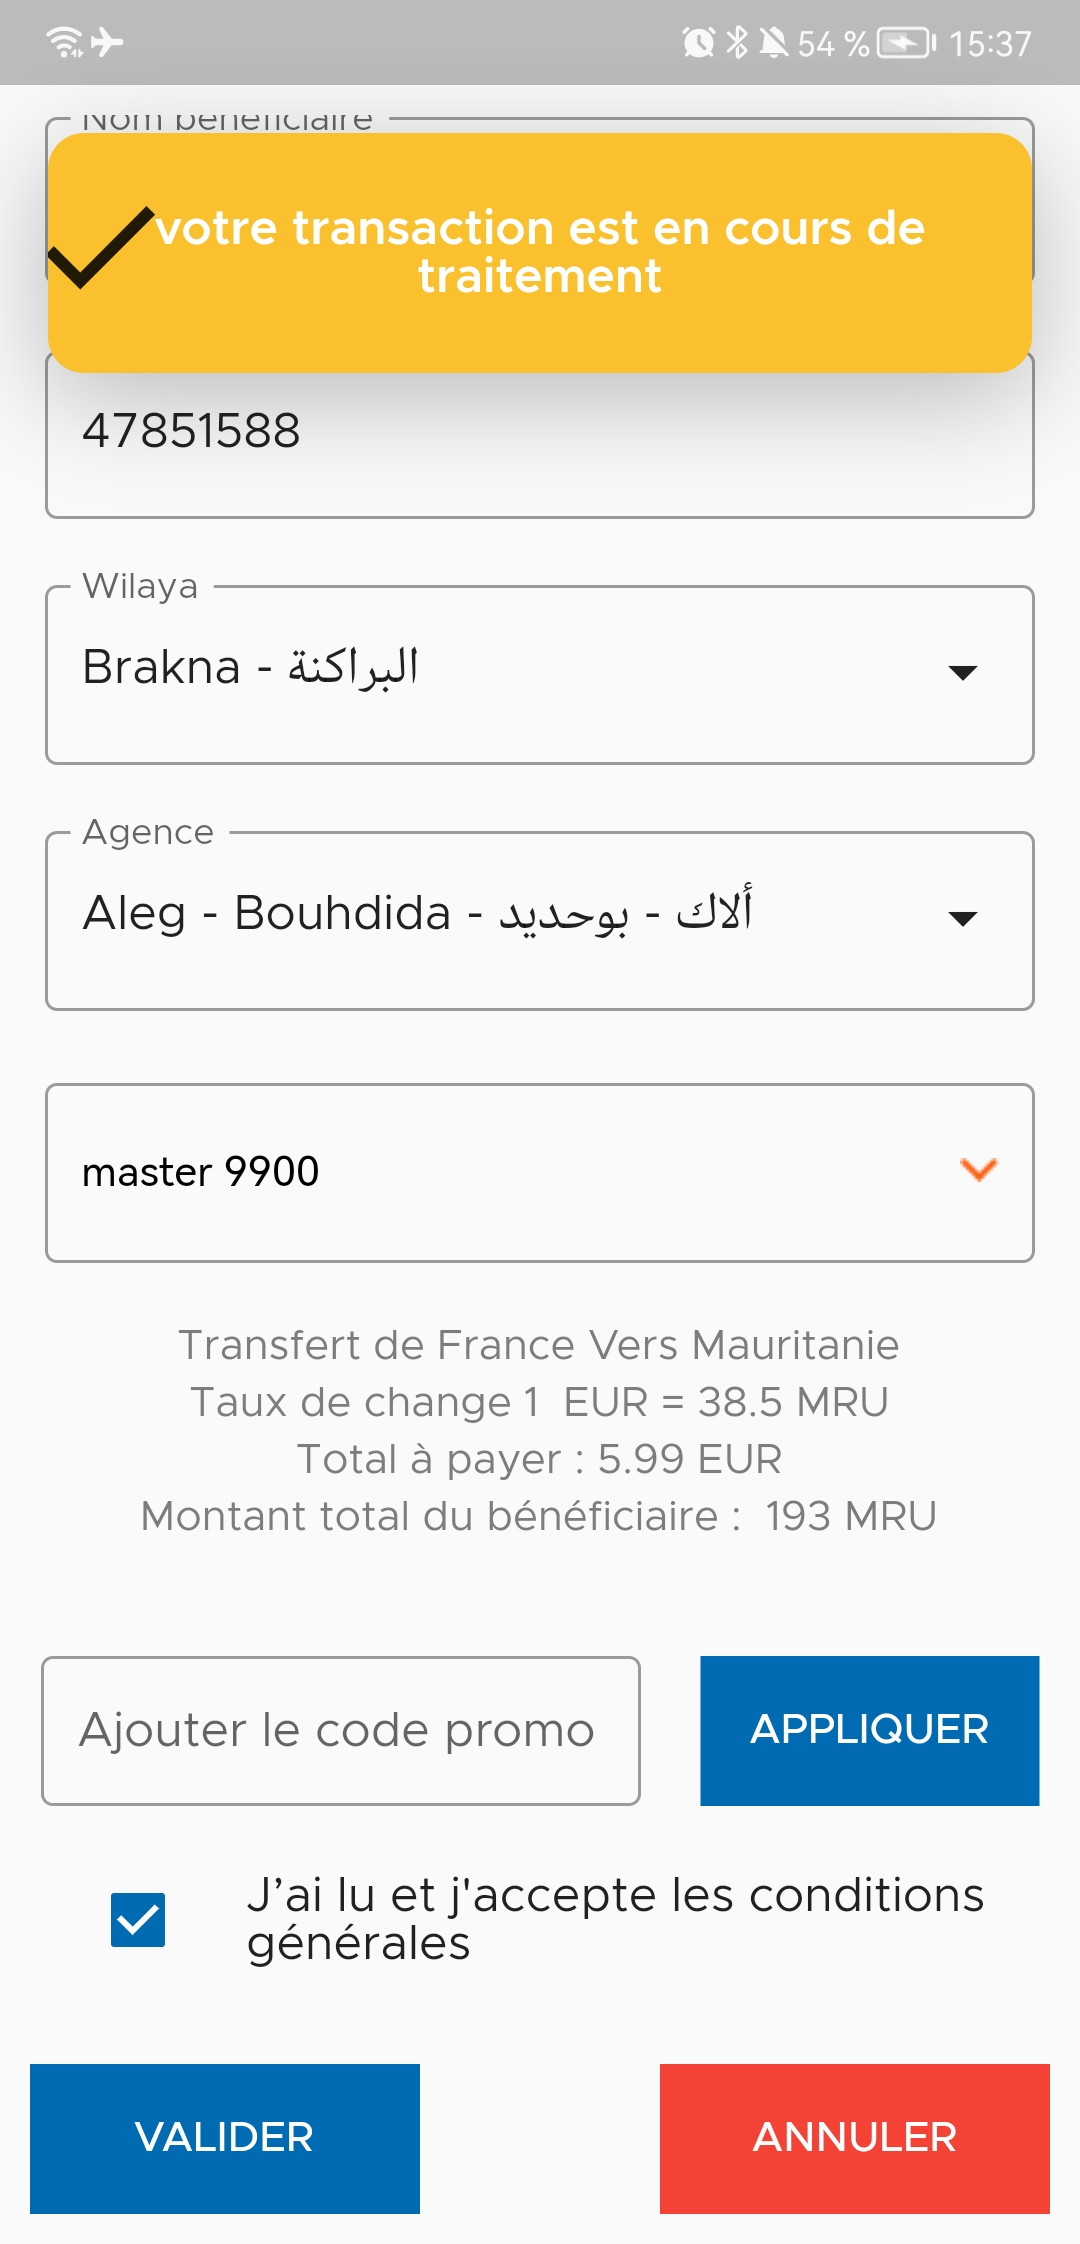
\includegraphics[width=\textwidth]{./Template LaTeX/Images/15.jpg}
		\caption{État de transfert}
		\label{fig:five over x}
	\end{subfigure}
	\caption{Processus de transactions}
	\label{fig:three graphs}
\end{figure}
\newpage
\item \textbf{L’interface de transfert
	:}La figure~\ref{transfert} montre l'historique des transactions de l'utilisateur  vers les bénéficiaires avec détails pour chaque transaction.

\begin{figure}
	\centering
	\begin{subfigure}[b]{0.3\textwidth}
		\centering
		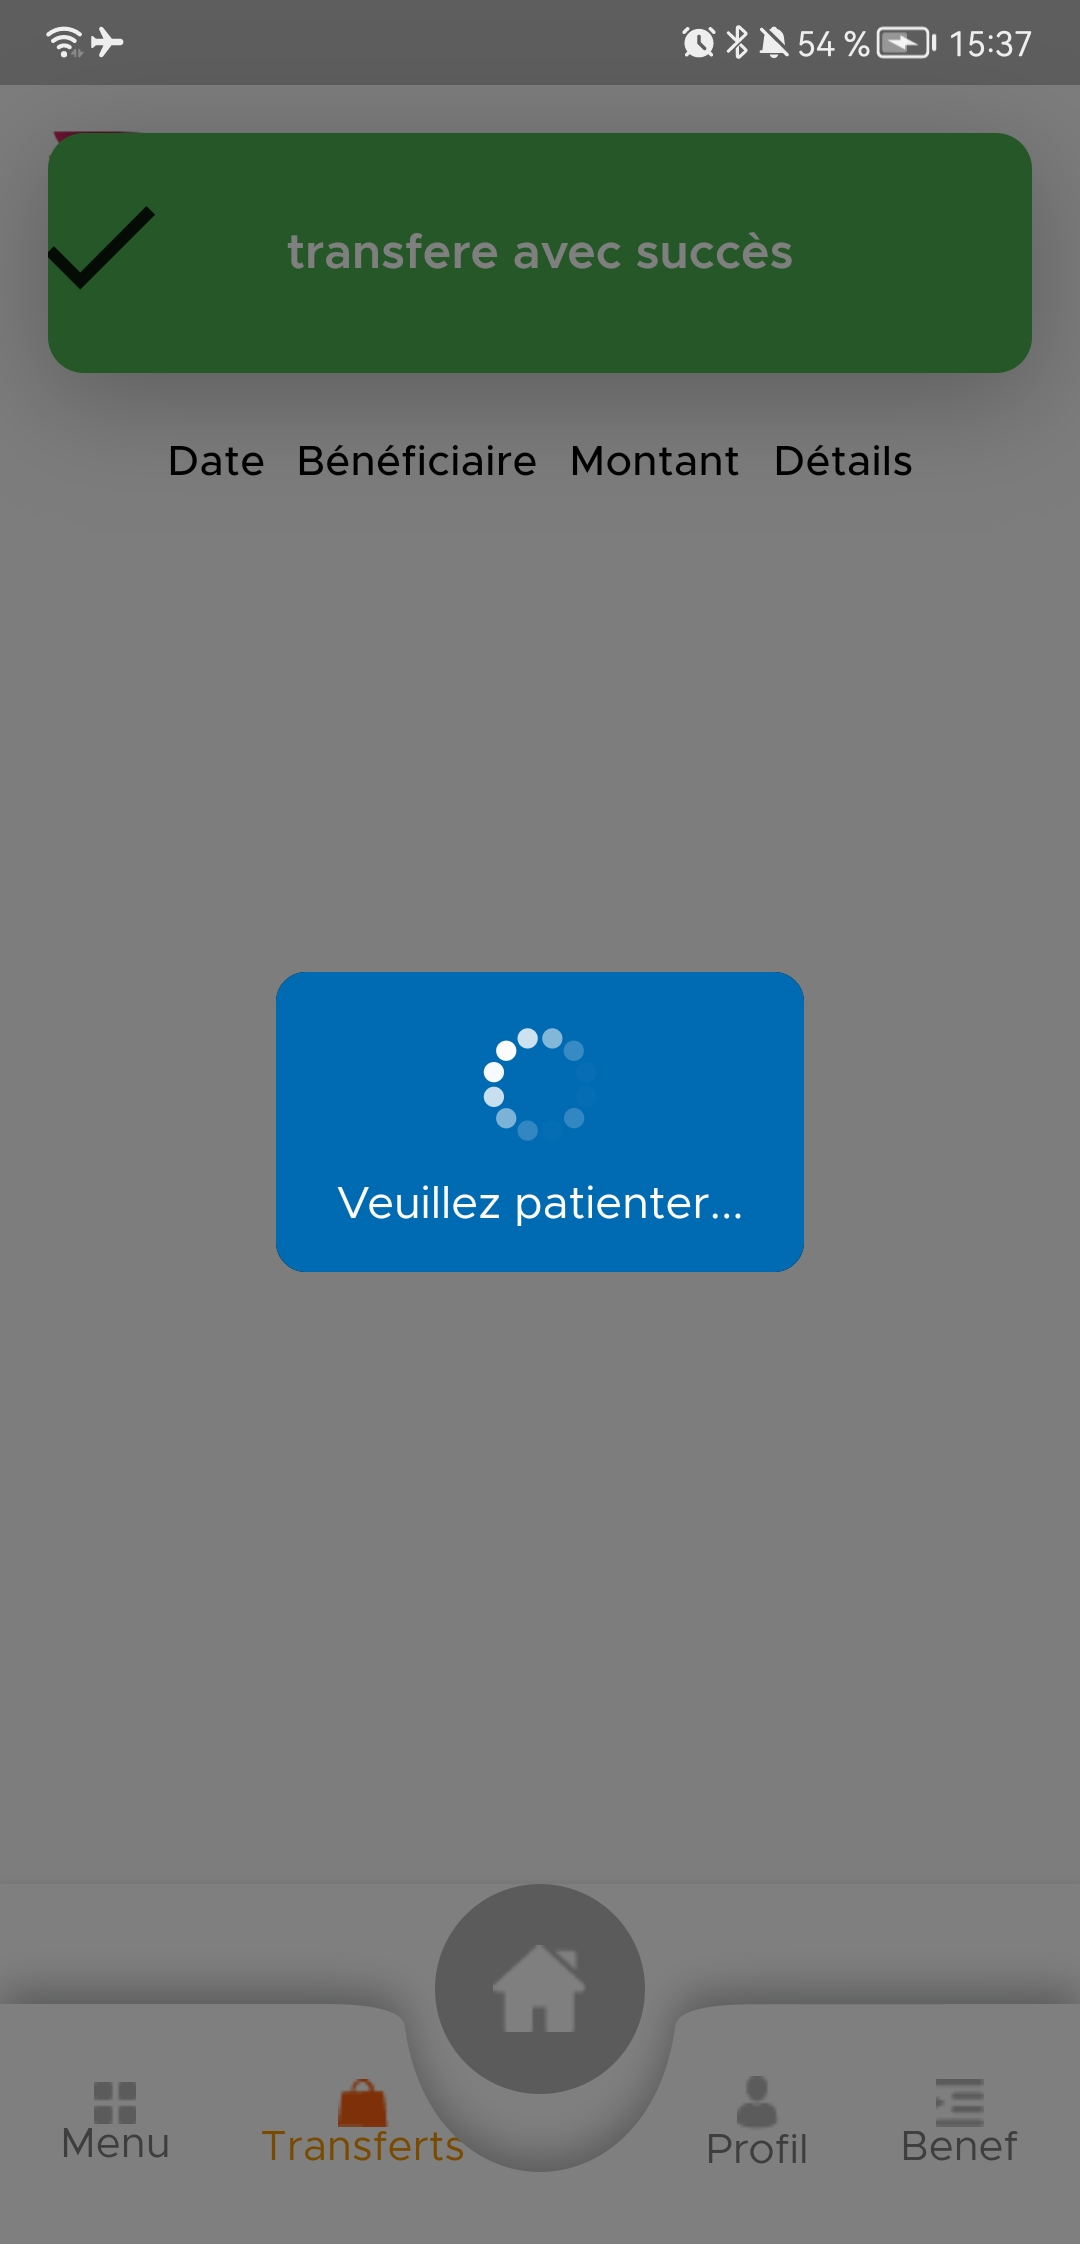
\includegraphics[width=\textwidth]{./Template LaTeX/Images/16.jpg}
		\caption{Transfere avec succés}
		\label{fig:y equals x}
	\end{subfigure}
	\hfill
	\begin{subfigure}[b]{0.3\textwidth}
		\centering
		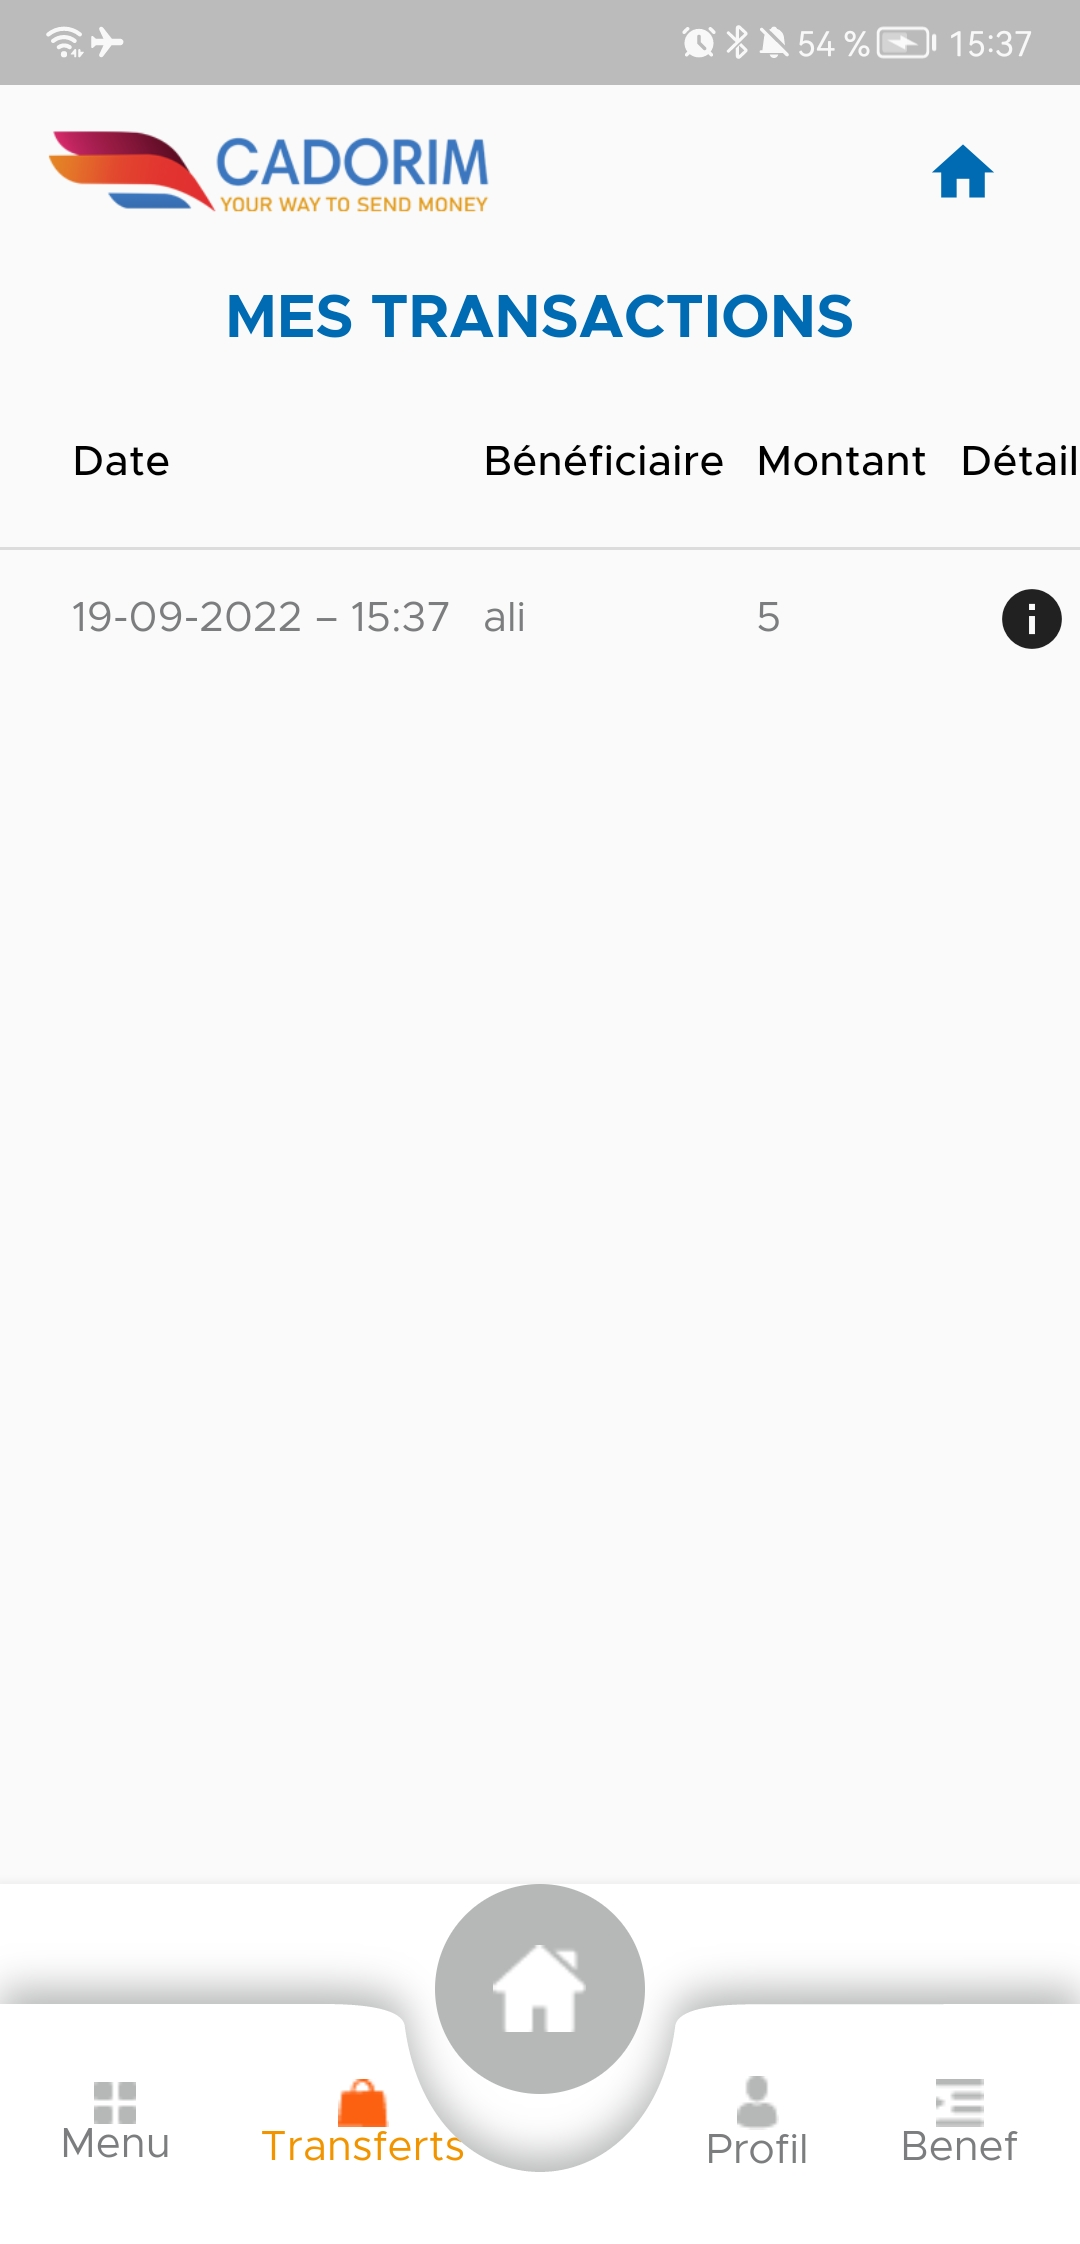
\includegraphics[width=\textwidth]{./Template LaTeX/Images/17.jpg}
		\caption{Historique transactions}
		\label{fig:three sin x}
	\end{subfigure}
	\hfill
	\begin{subfigure}[b]{0.3\textwidth}
		\centering
		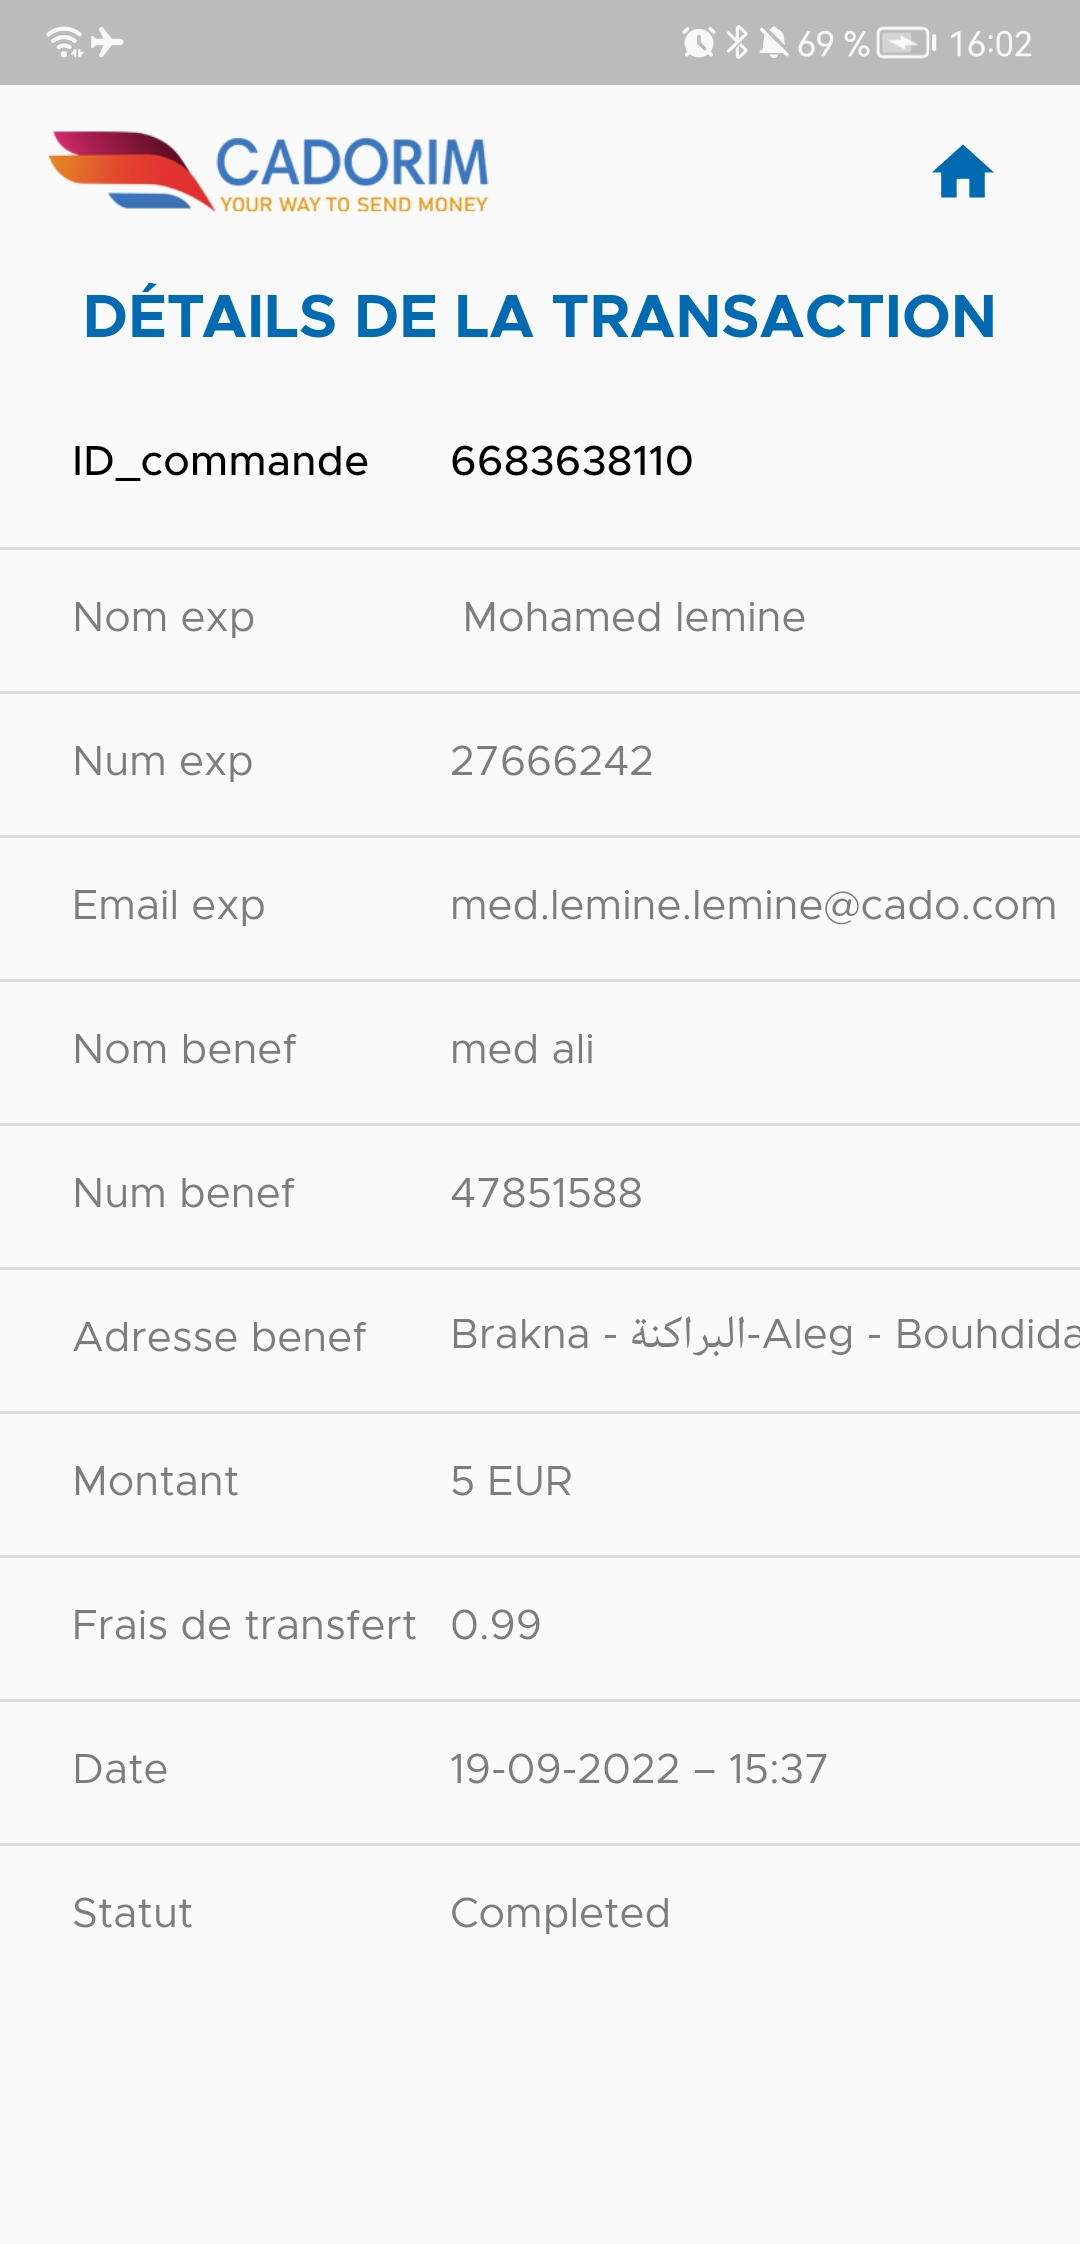
\includegraphics[width=\textwidth]{./Template LaTeX/Images/18.jpg}
		\caption{Détails de la transaction}
		\label{fig:five over x}
	\end{subfigure}
	\caption{Transferts}
	\label{transfert}
\end{figure}

\item \textbf{L’interface de discussion
	:} La figure suivante montre que le client peut envoyer un message (photo ou un texte) au service client et bien sur voir l'historique des messages.
	\begin{figure}%
	\centering
	{{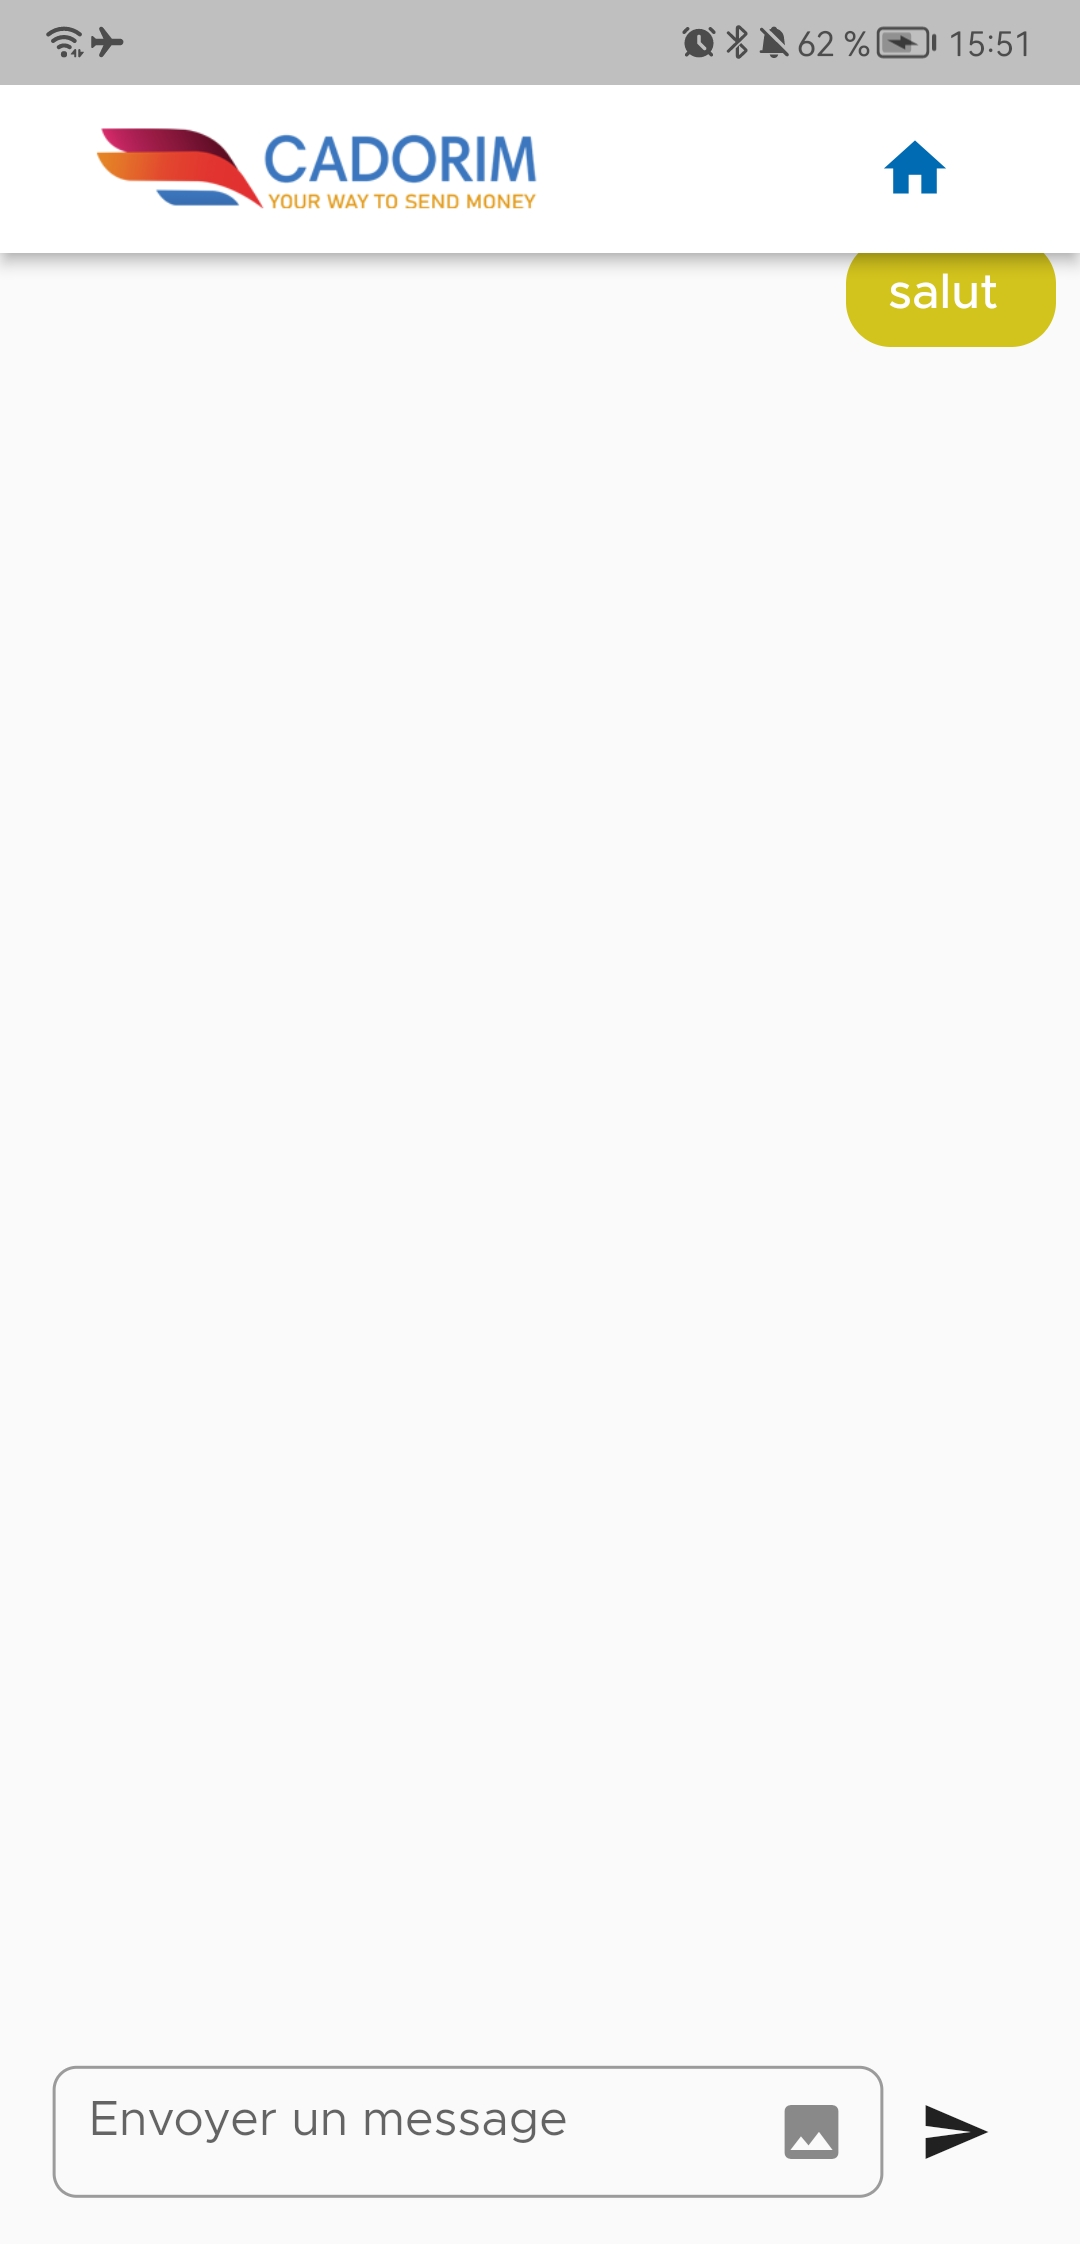
\includegraphics[width=5cm]{./Template LaTeX/Images/21.jpg} }}%
	\caption{Interface de discussion}%
	\label{fig:example}%
\end{figure}
\newpage
\item \textbf{Profil de l'utilisateur:} L'utilisateur peut mettre à jour leur profil ou ajouter un mode paiement comme il montre la figure suivante
\begin{figure}
	\centering
	\begin{subfigure}[b]{0.3\textwidth}
		\centering
		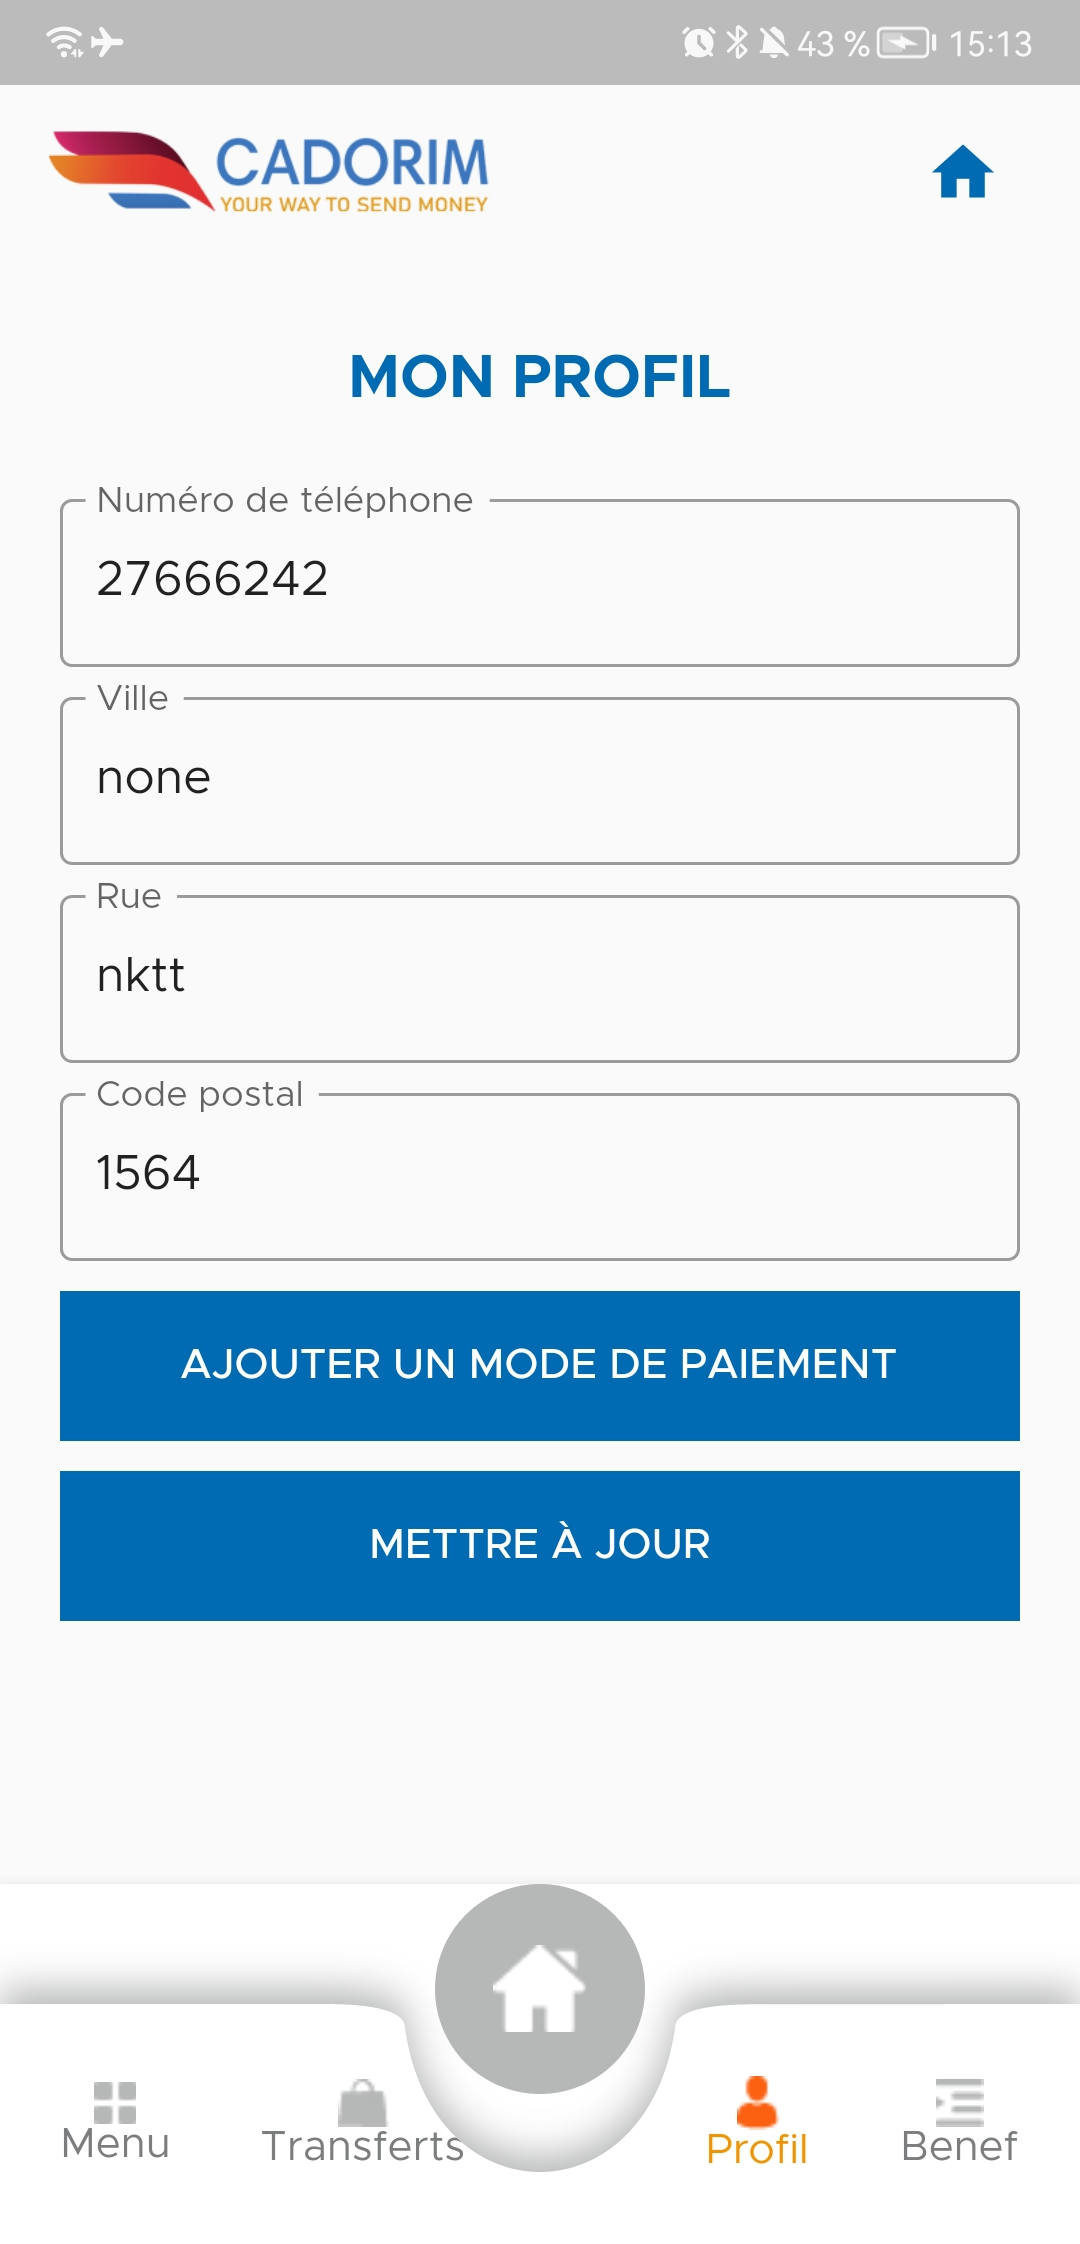
\includegraphics[width=\textwidth]{./Template LaTeX/Images/6.jpg}
		\caption{Mon profil}
		\label{fig:y equals x}
	\end{subfigure}
	\hfill
	\begin{subfigure}[b]{0.3\textwidth}
		\centering
		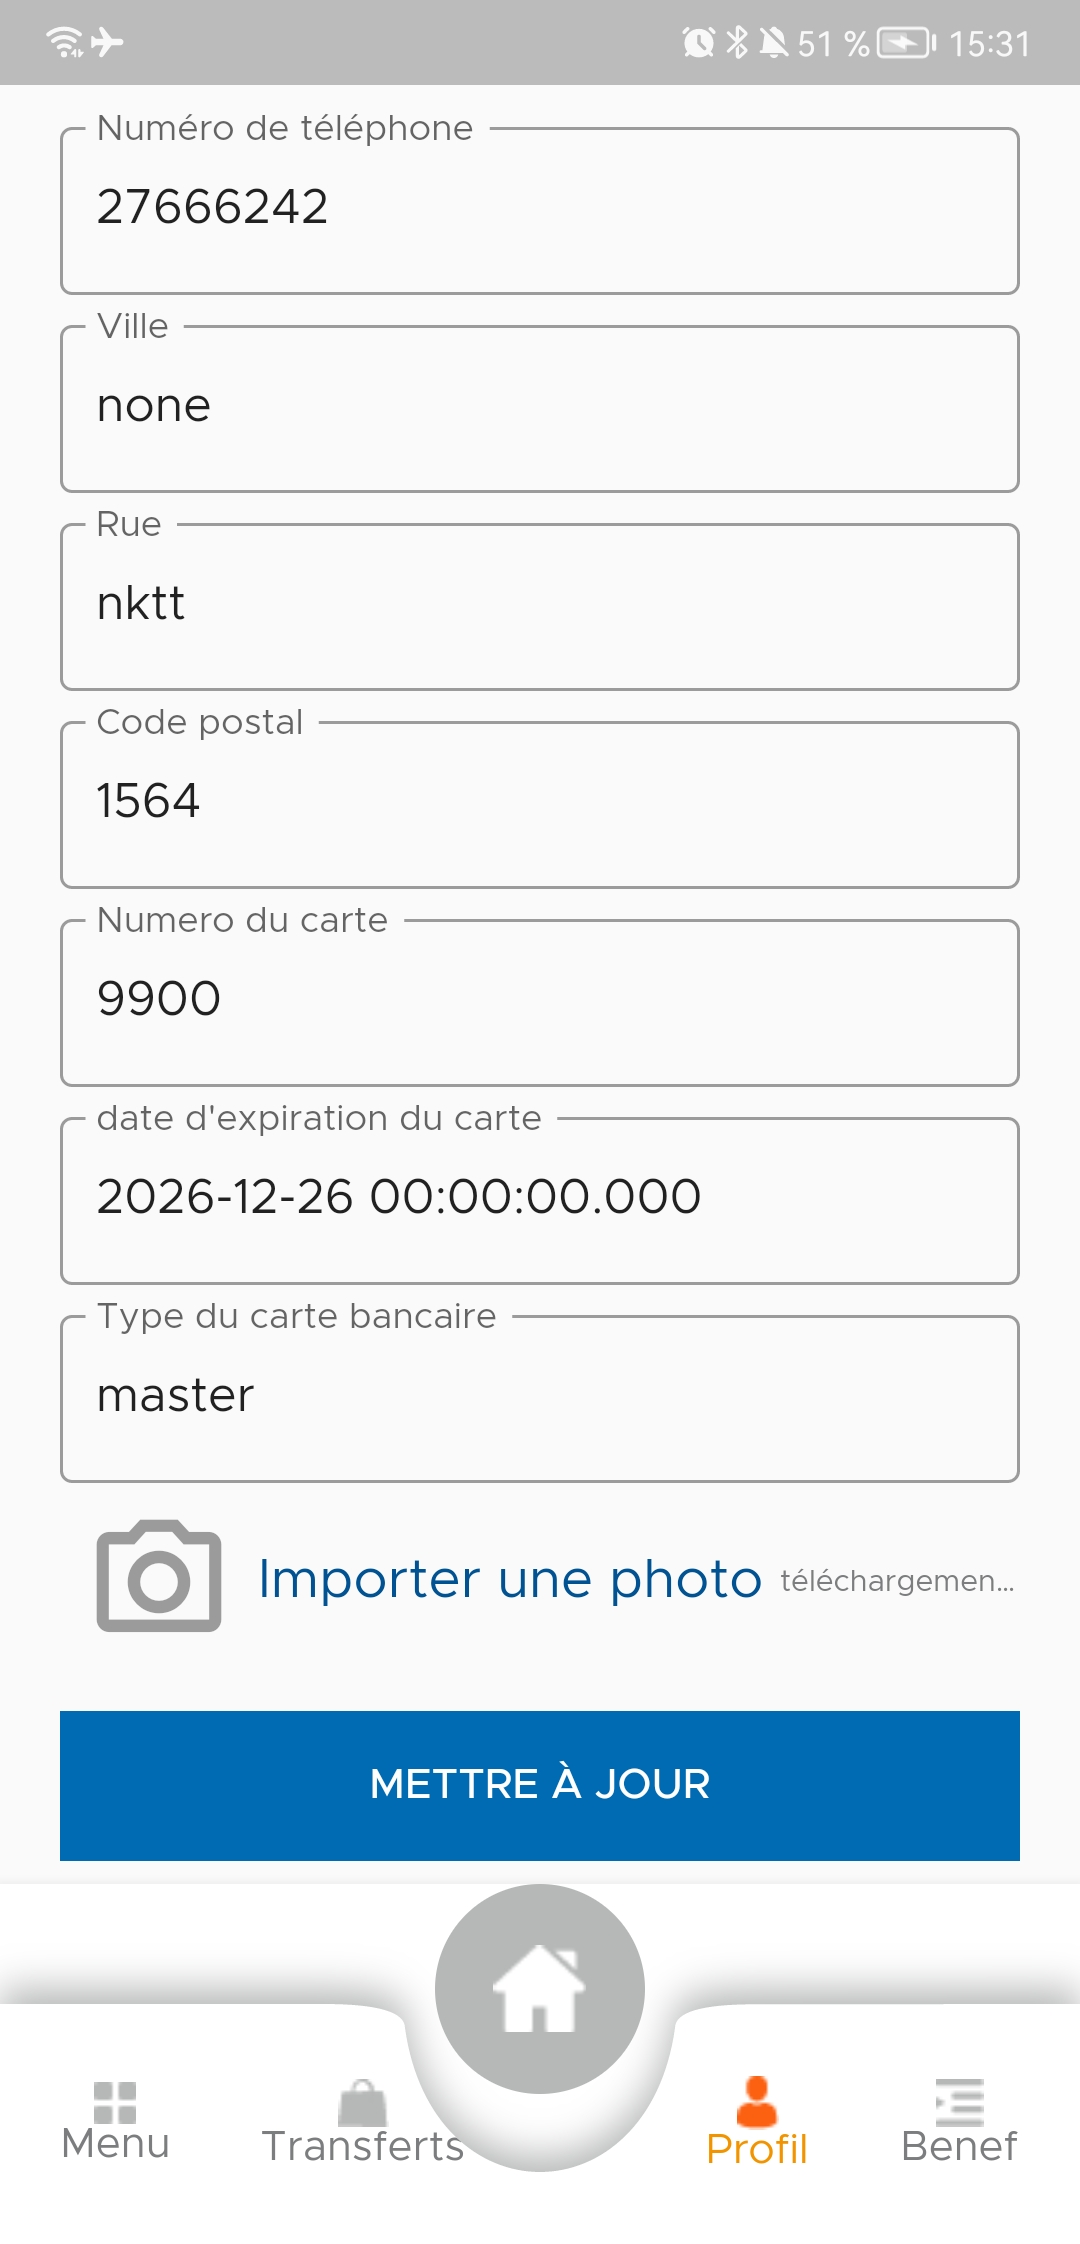
\includegraphics[width=\textwidth]{./Template LaTeX/Images/7.jpg}
		\caption{Ajouter une carte}
		\label{fig:three sin x}
	\end{subfigure}
	\hfill
	\begin{subfigure}[b]{0.3\textwidth}
		\centering
		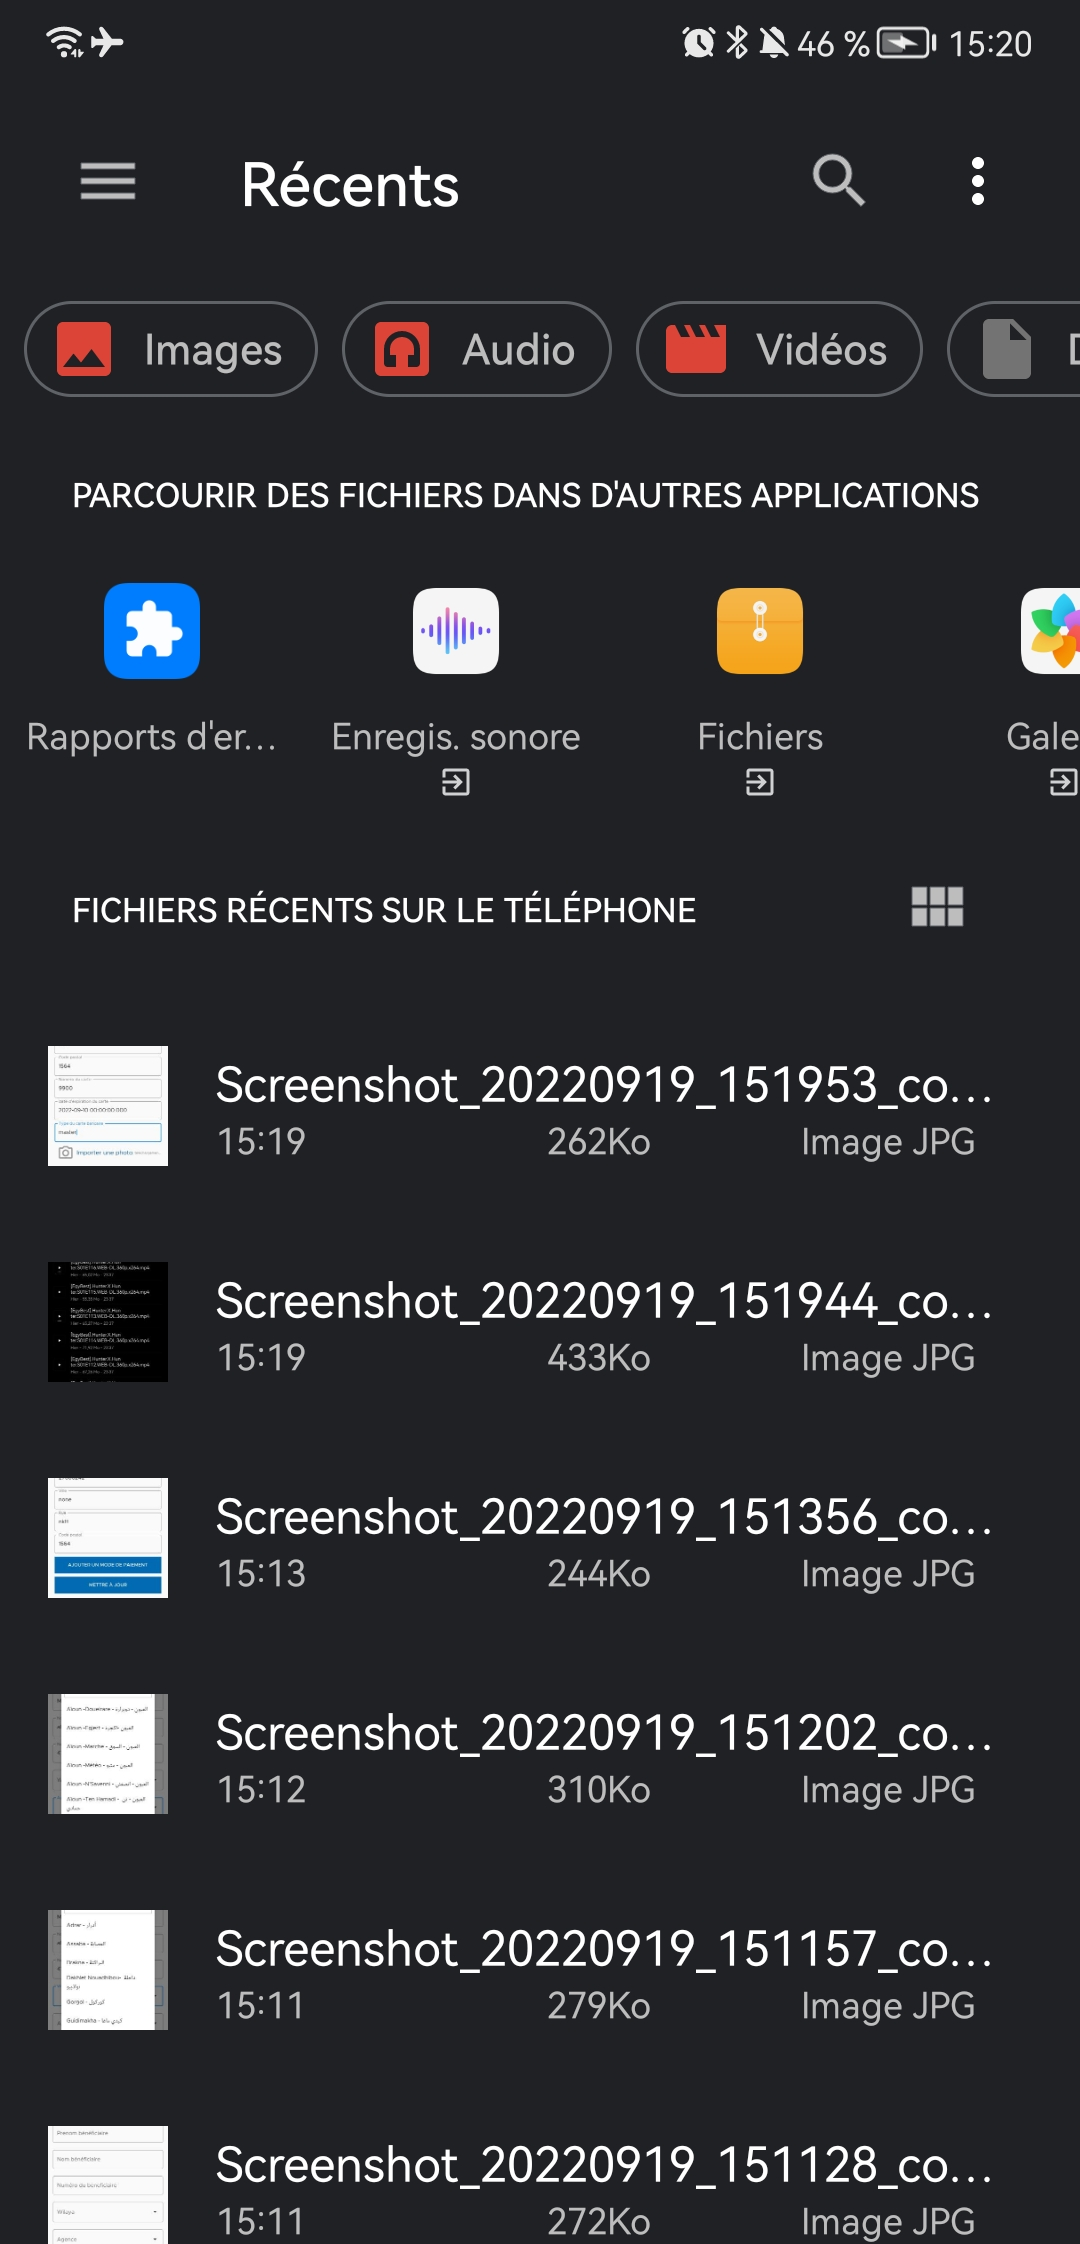
\includegraphics[width=\textwidth]{./Template LaTeX/Images/8.jpg}
		\caption{Importer une photo}
		\label{fig:five over x}
	\end{subfigure}
\newline
	\centering
\begin{subfigure}{0.3\textwidth}
	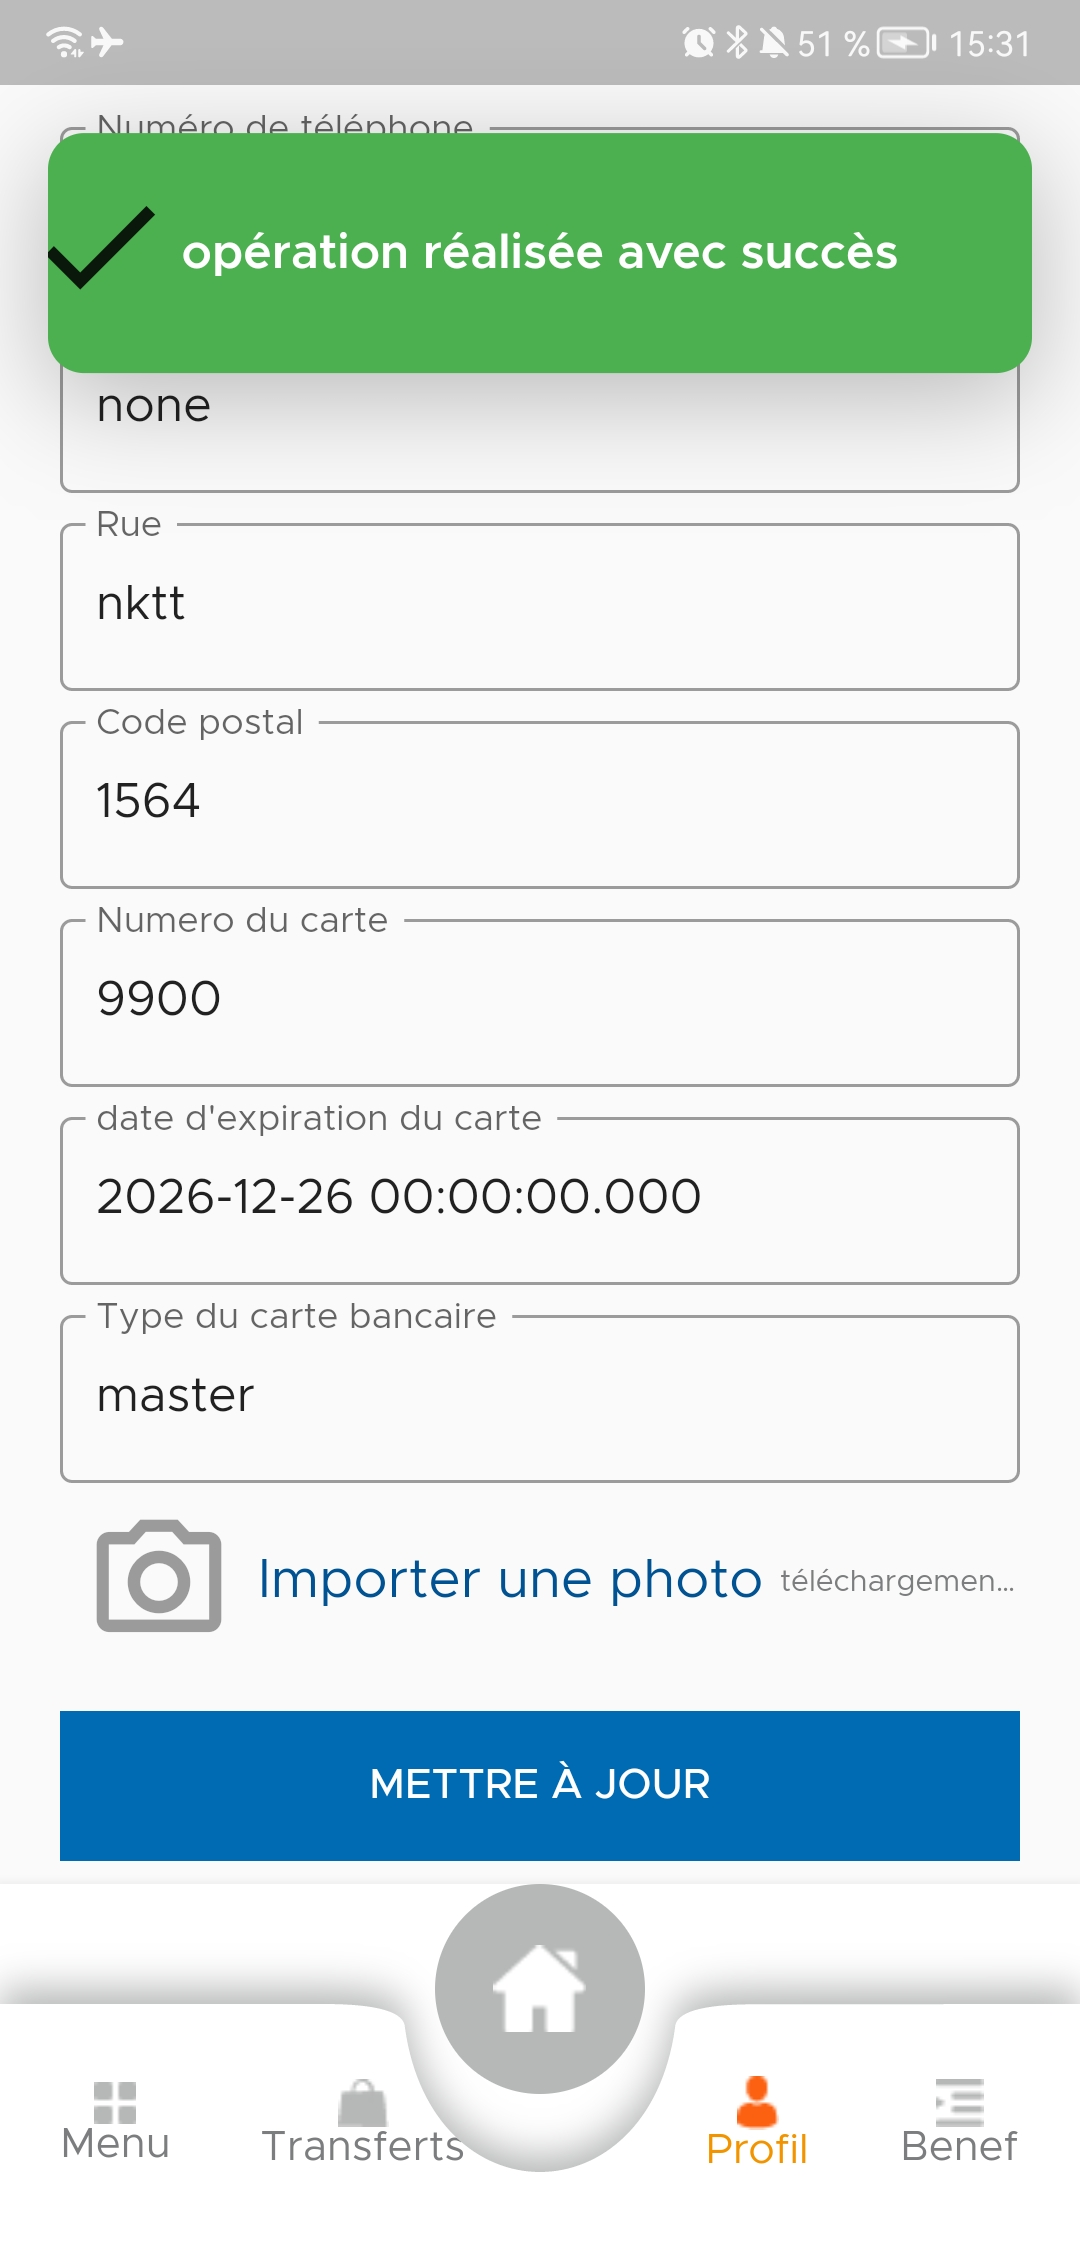
\includegraphics[width=\hsize, valign=m ]{./Template LaTeX/Images/9.jpg}
	\caption{État}
	\label{fig.SICAPI}
\end{subfigure}
%\qquad\tikz[baseline=-\baselineskip]\draw[ultra thick,->] (0,0) -- ++ (1,0);\qquad
\begin{subfigure}{0.3\textwidth}
	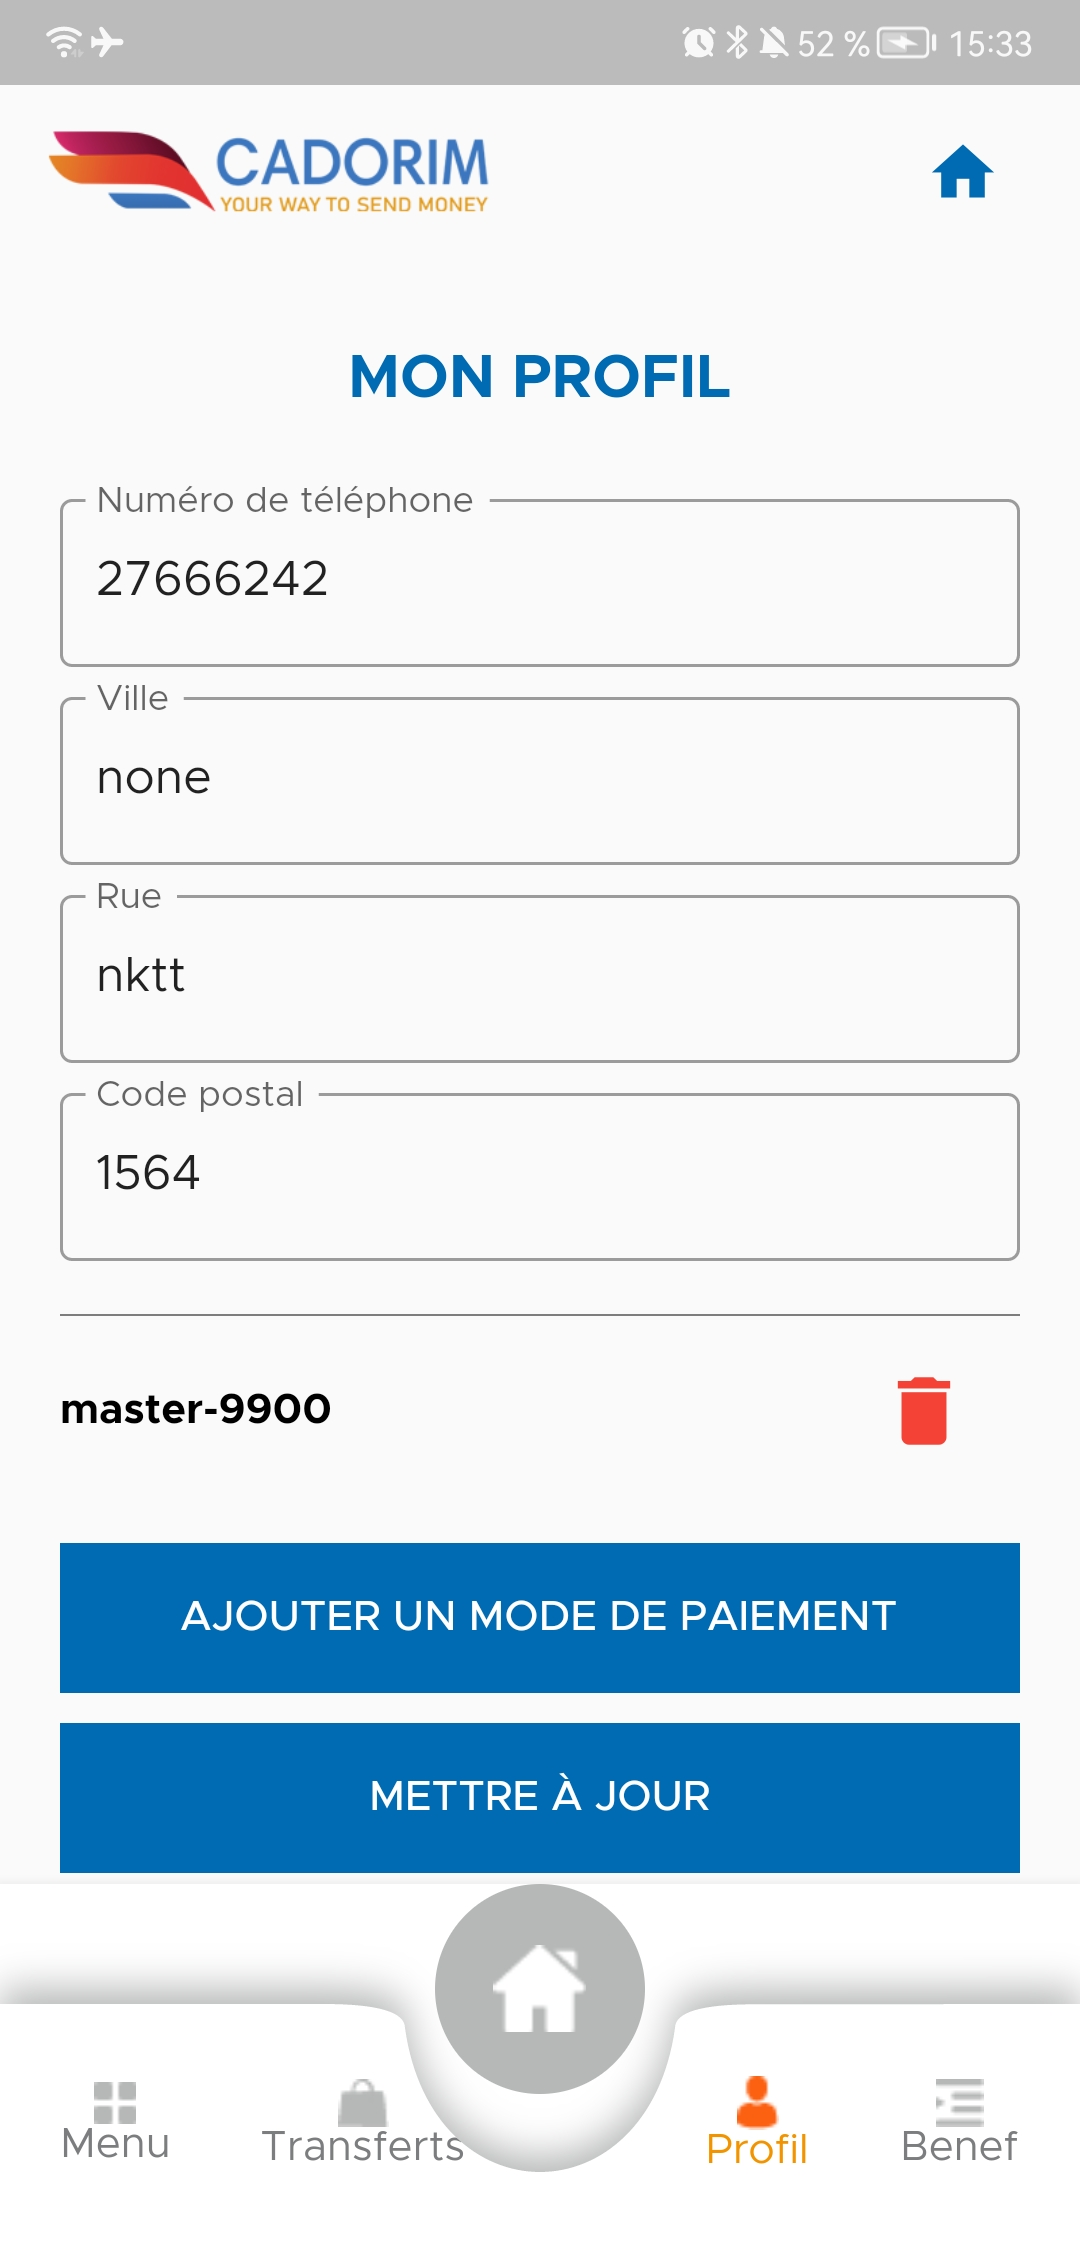
\includegraphics[width=\hsize, valign=m]{./Template LaTeX/Images/10.jpg}
	\caption{Interface suivante}
	\label{fig.painel_sicapi}
\end{subfigure}
	\caption{Profil de l'utilisateur
	}
	\label{fig:three graphs}
\end{figure}


%%%%%%%%%%%%%%%%%%%%%%%%%%%%%%%%MENU%%%%%%%%%%%%%%%%%%%%%%%%%%%%%%%
\newpage
\item \textbf{L’interface de menu
	:} À partir de cette fenêtre le client a l'accès aux autres fonctionalistes de l'application (Modifier mot de passe,changer la langue ....)
\begin{figure}%
	\centering
	{{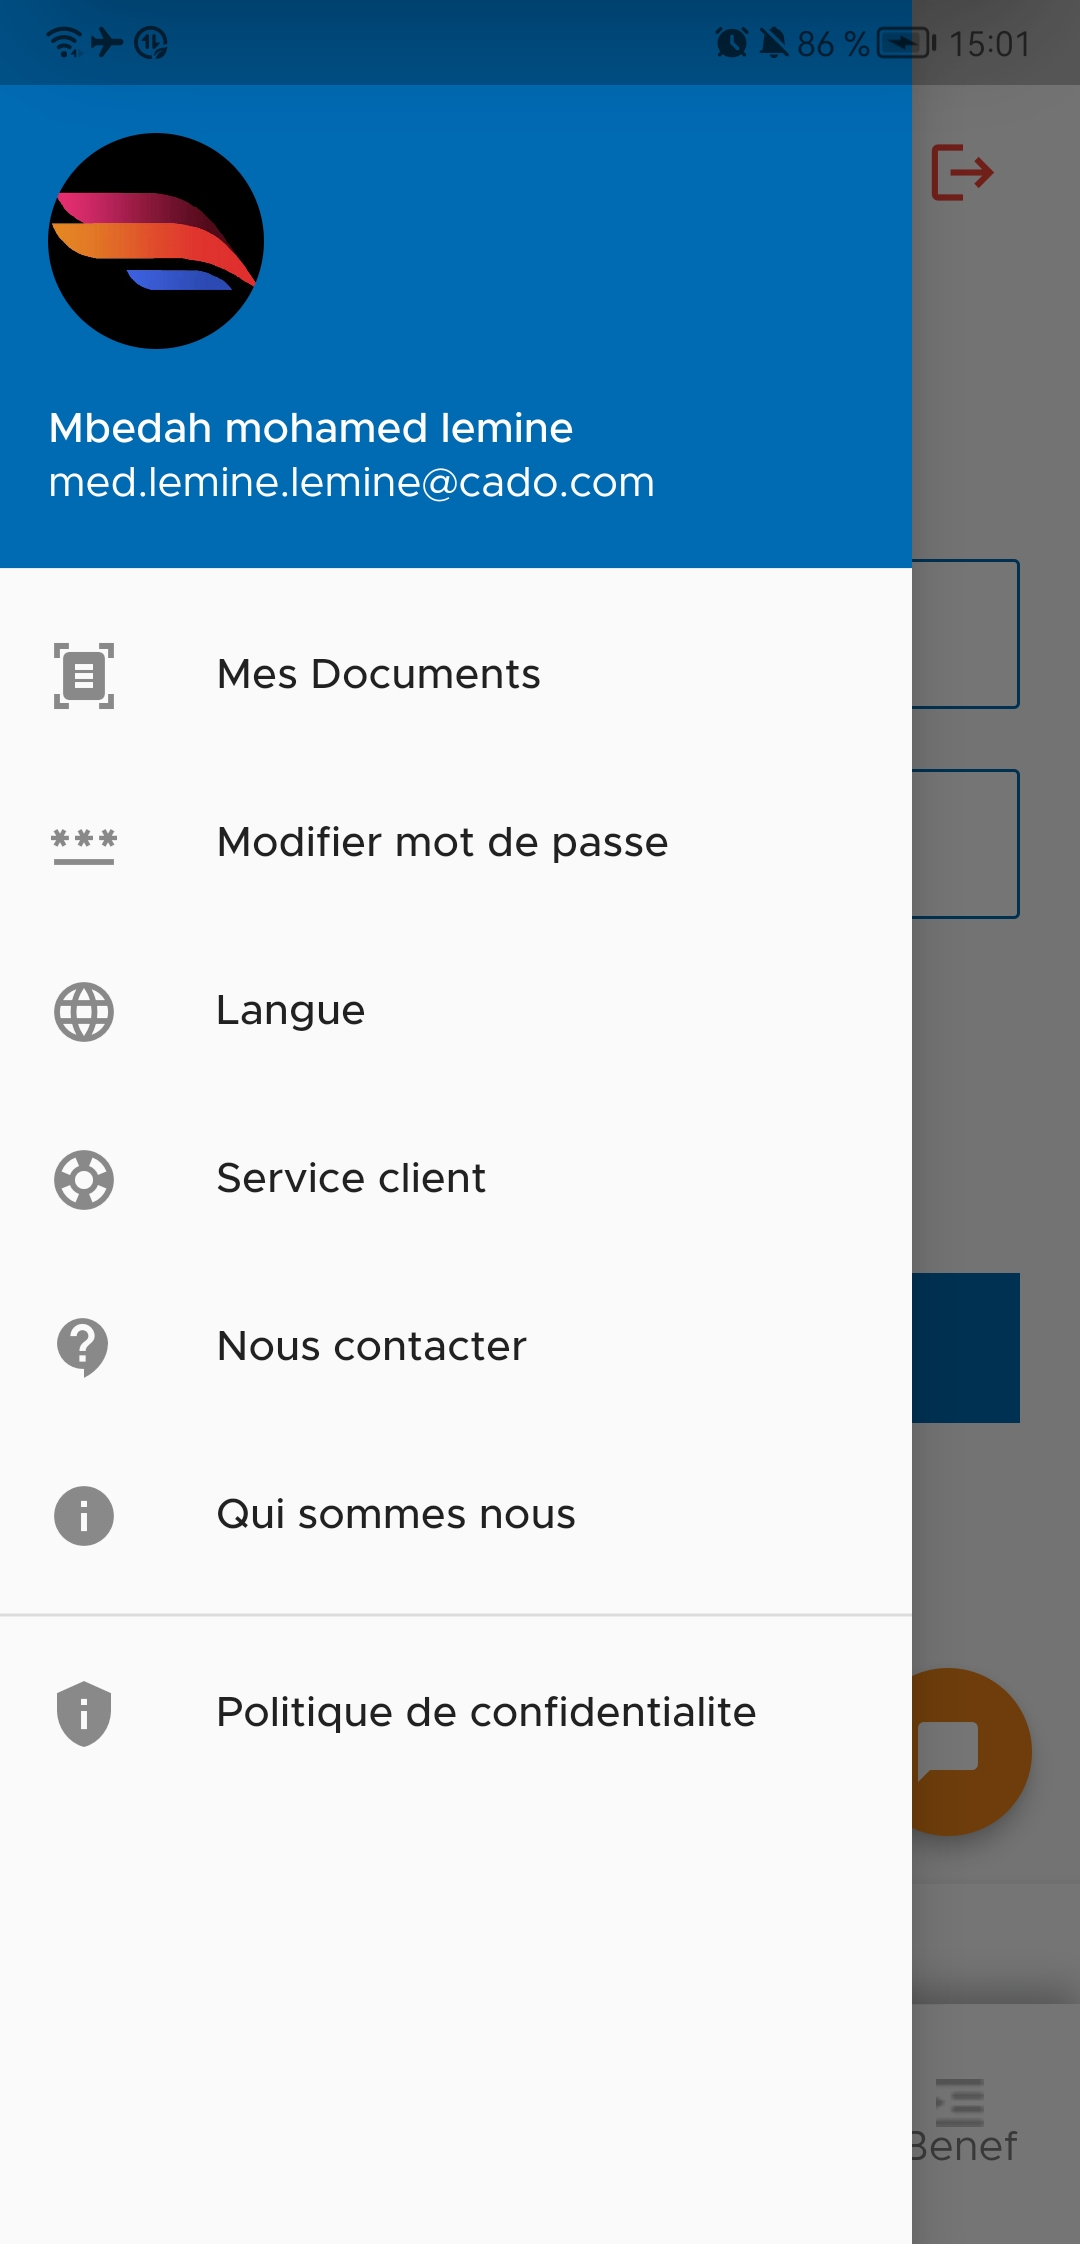
\includegraphics[width=5cm]{./Template LaTeX/Images/22.jpg} }}%
	\caption{Interface de menu}%
	\label{fig:example}%
\end{figure}
\end{itemize}

\subsubsection{Application ServiceClient}
\begin{itemize}[label=$\ast$]
		\item \textbf{L’interface
		d’authentification
		:} La figure suivante représente l’interface d’authentification de notre application. Elle permet aux utilisateurs de s’identifier en introduisant leurs identifiants afin d’accéder aux fonctionnalités de l’application.
	
	\begin{figure}%
		\centering
		{{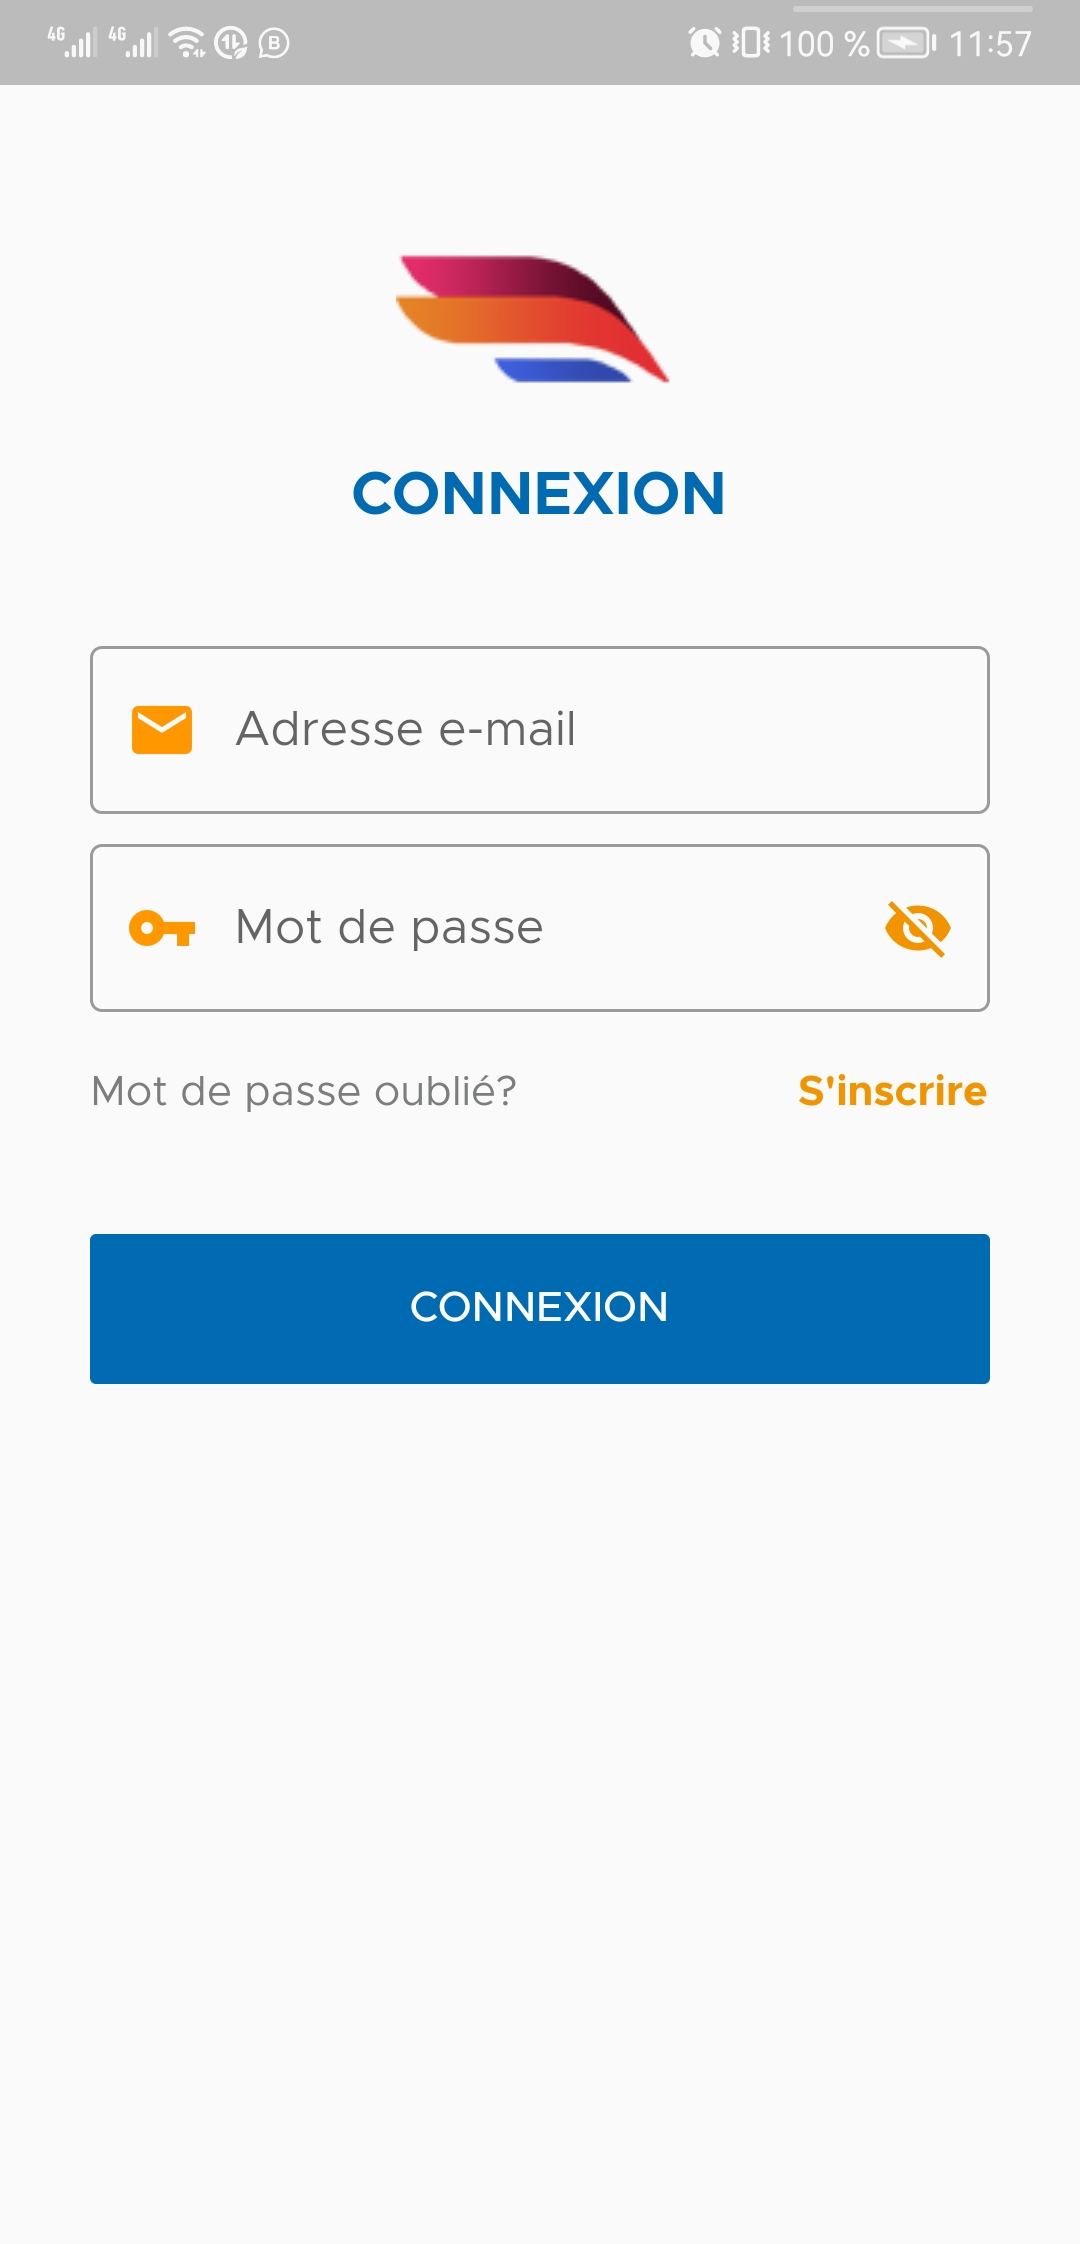
\includegraphics[width=5cm]{./Template LaTeX/Images/3.jpg} }}%
		\caption{Interface d'authentification}%
		\label{fig:example}%
	\end{figure}
\newpage
	\item \textbf{L’interface du compte administrateur
	:} La figure~\ref{Home} représente la page principale de l’application pour l'administrateur. C’est à partir de cette fenêtre qu’est accessible la majorité des fonctionnalités de base de l’application(Gérer les comptes de service client).
\begin{comment}
	content...
}
\begin{figure}
	\centering
	\begin{subfigure}[b]{0.3\textwidth}
		\centering
		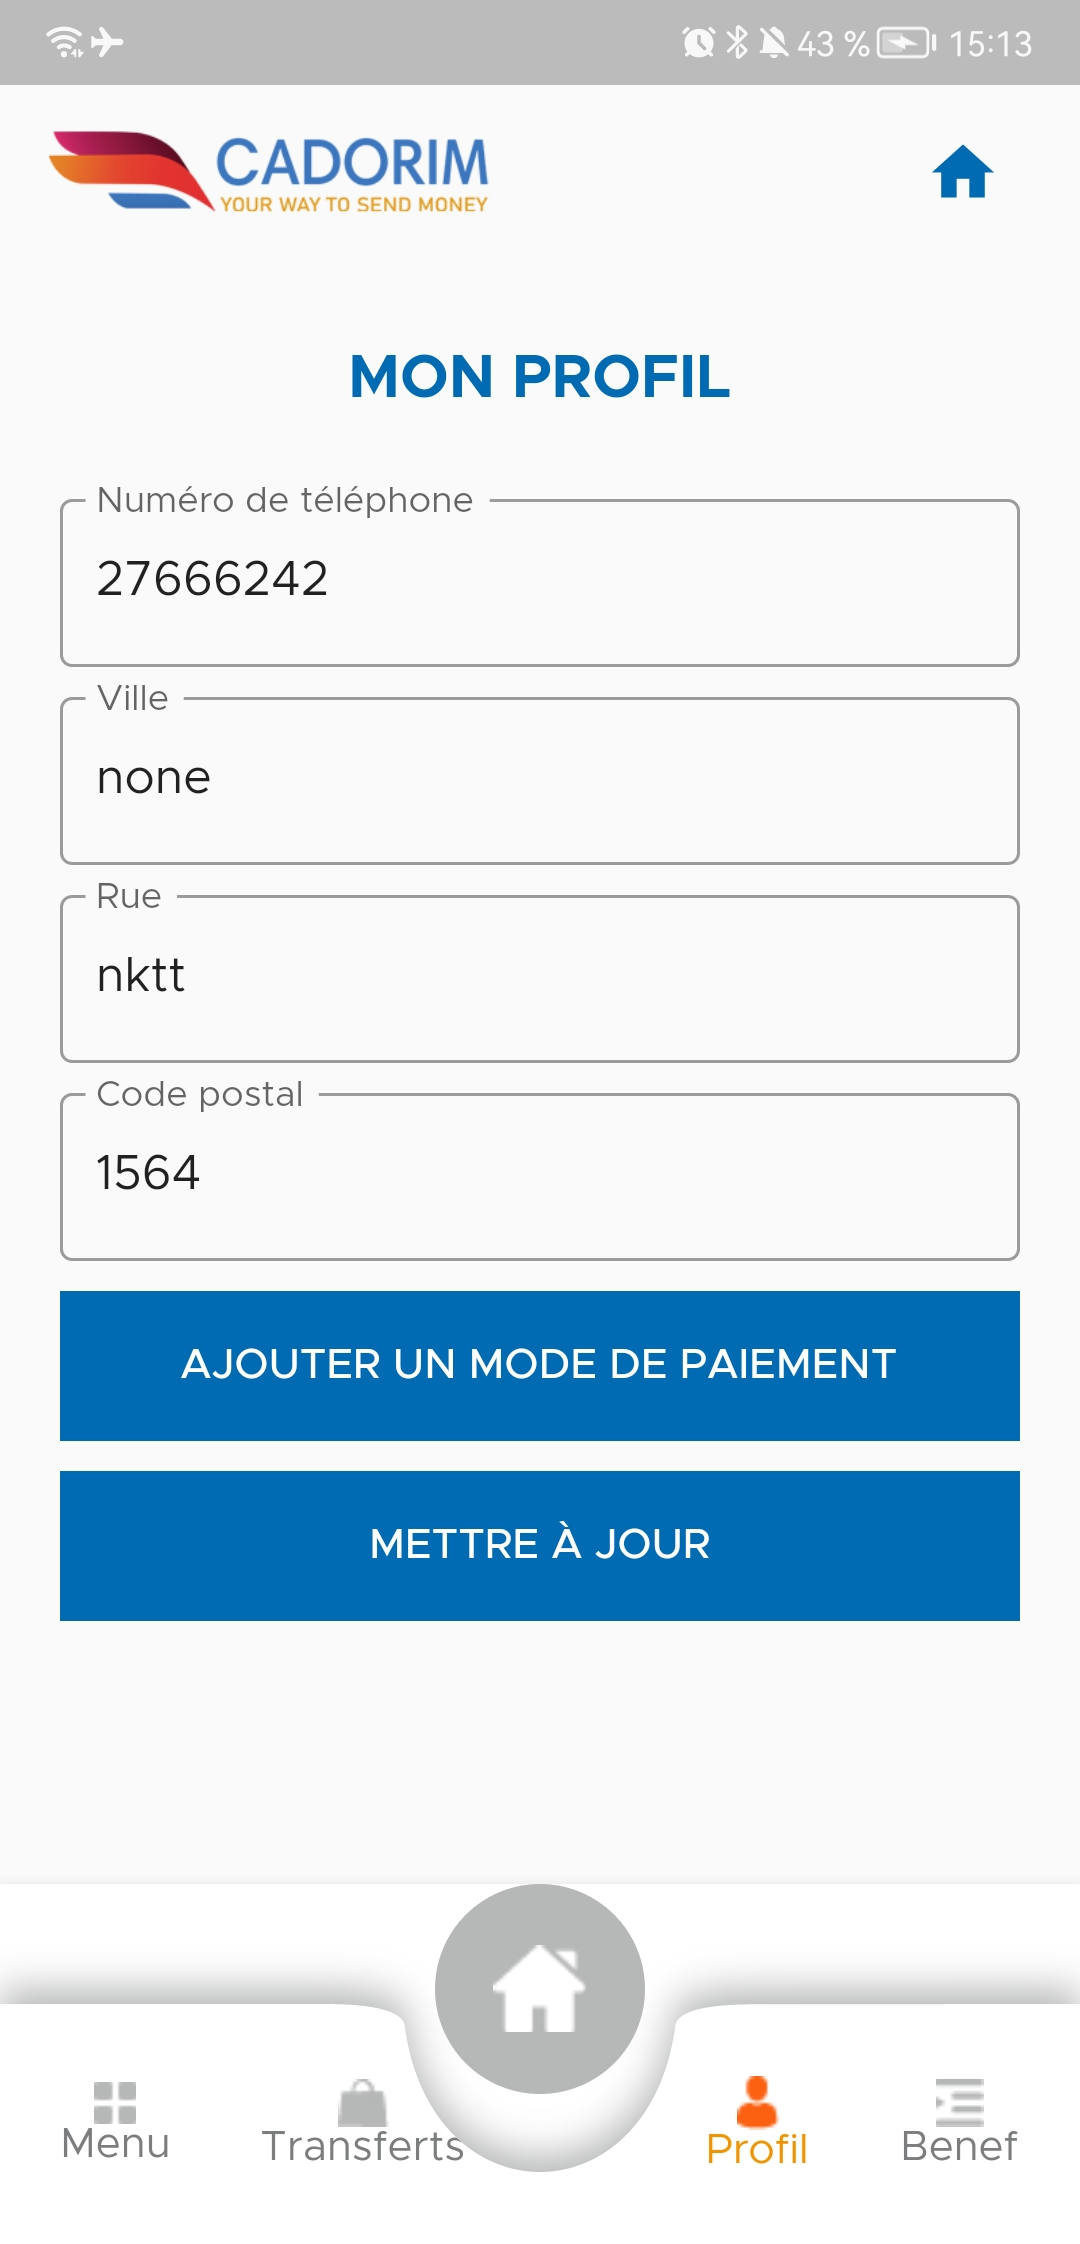
\includegraphics[width=\textwidth]{./Template LaTeX/Images/6.jpg}
		\caption{Interfaces d’accueil}
		\label{fig:y equals x}
	\end{subfigure}
	\hfill
	\begin{subfigure}[b]{0.3\textwidth}
		\centering
		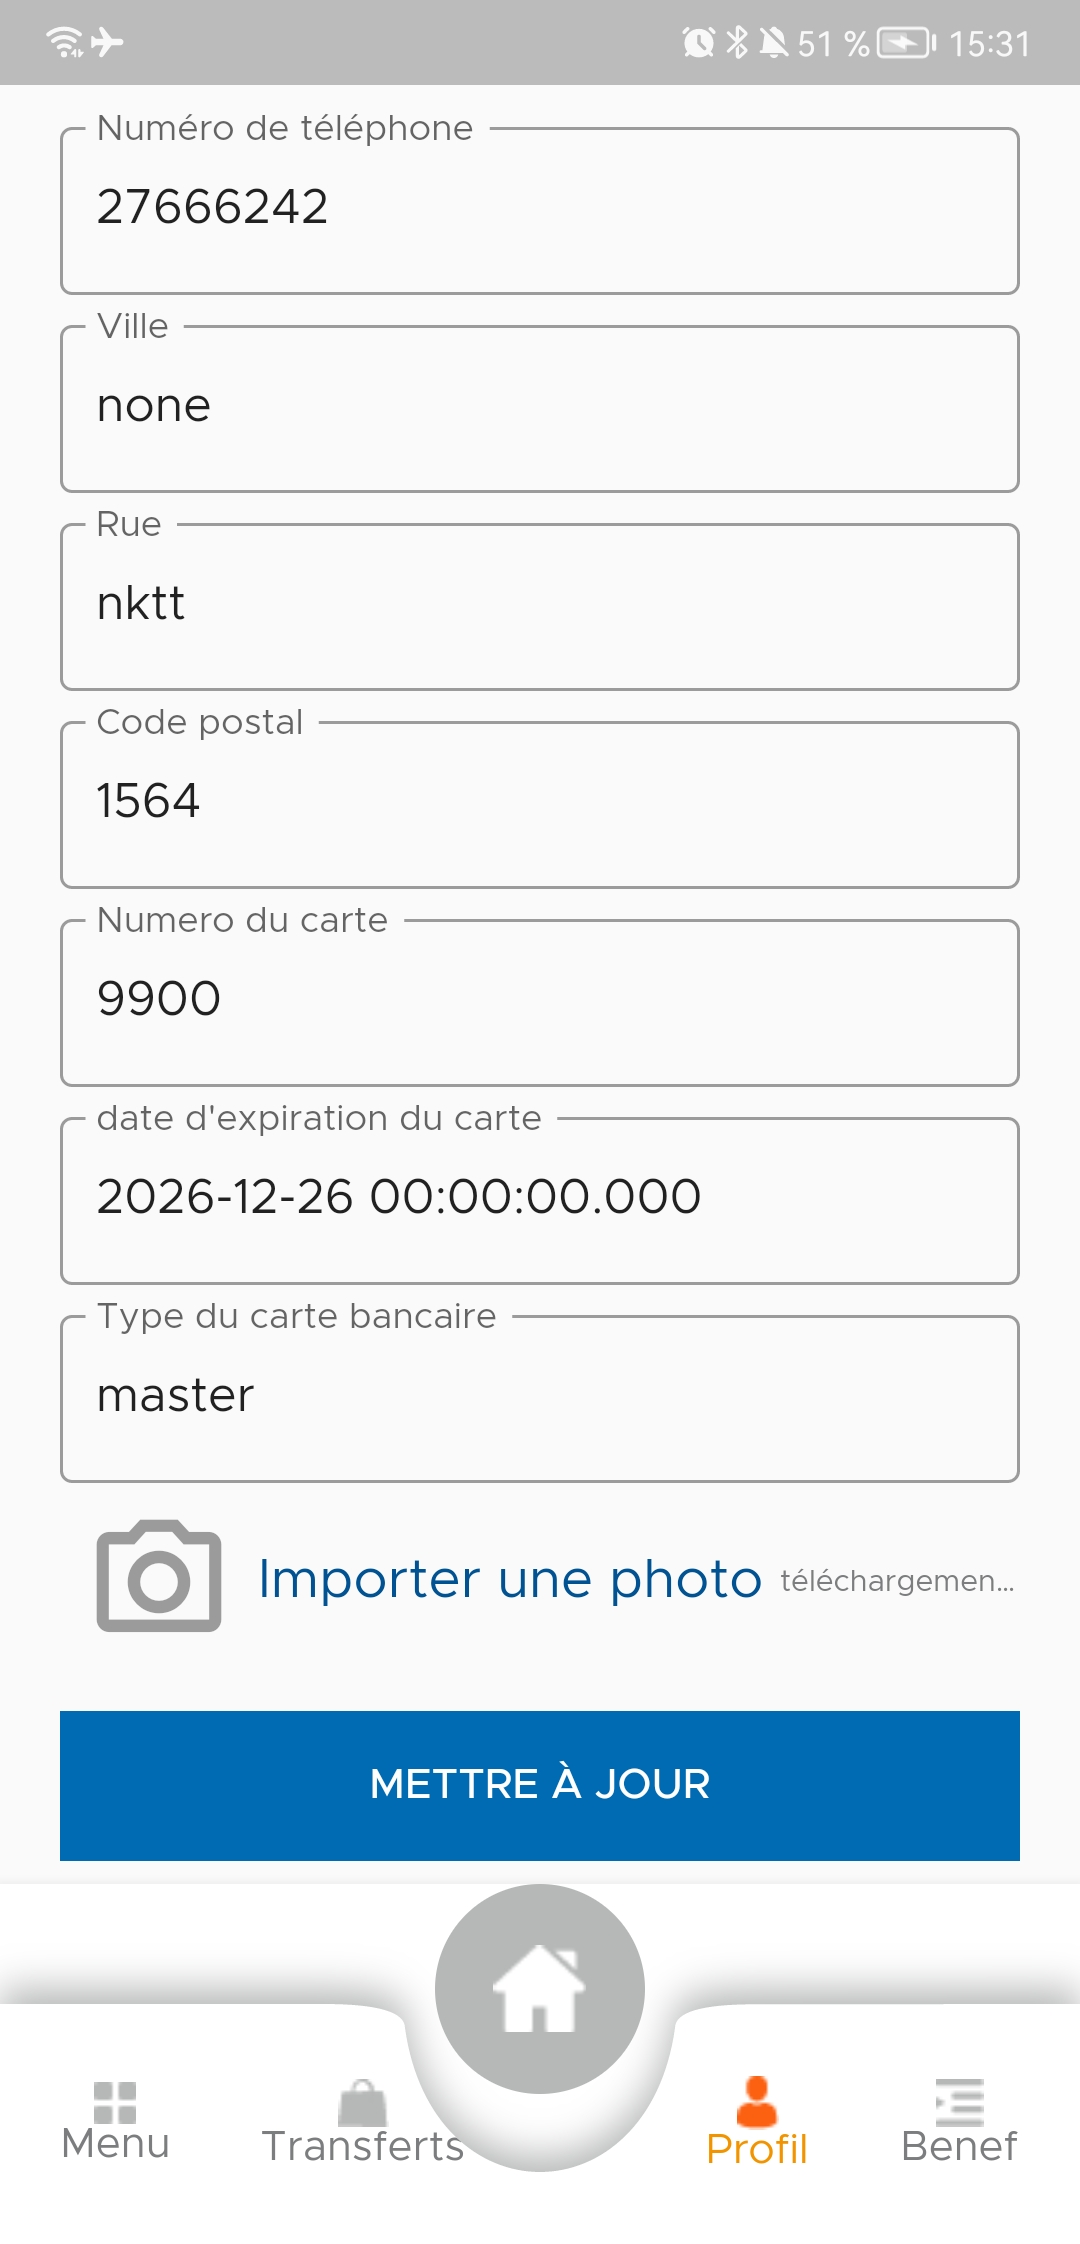
\includegraphics[width=\textwidth]{./Template LaTeX/Images/7.jpg}
		\caption{Supprimer un compte}
		\label{fig:three sin x}
	\end{subfigure}
	\hfill
	\begin{subfigure}[b]{0.3\textwidth}
		\centering
		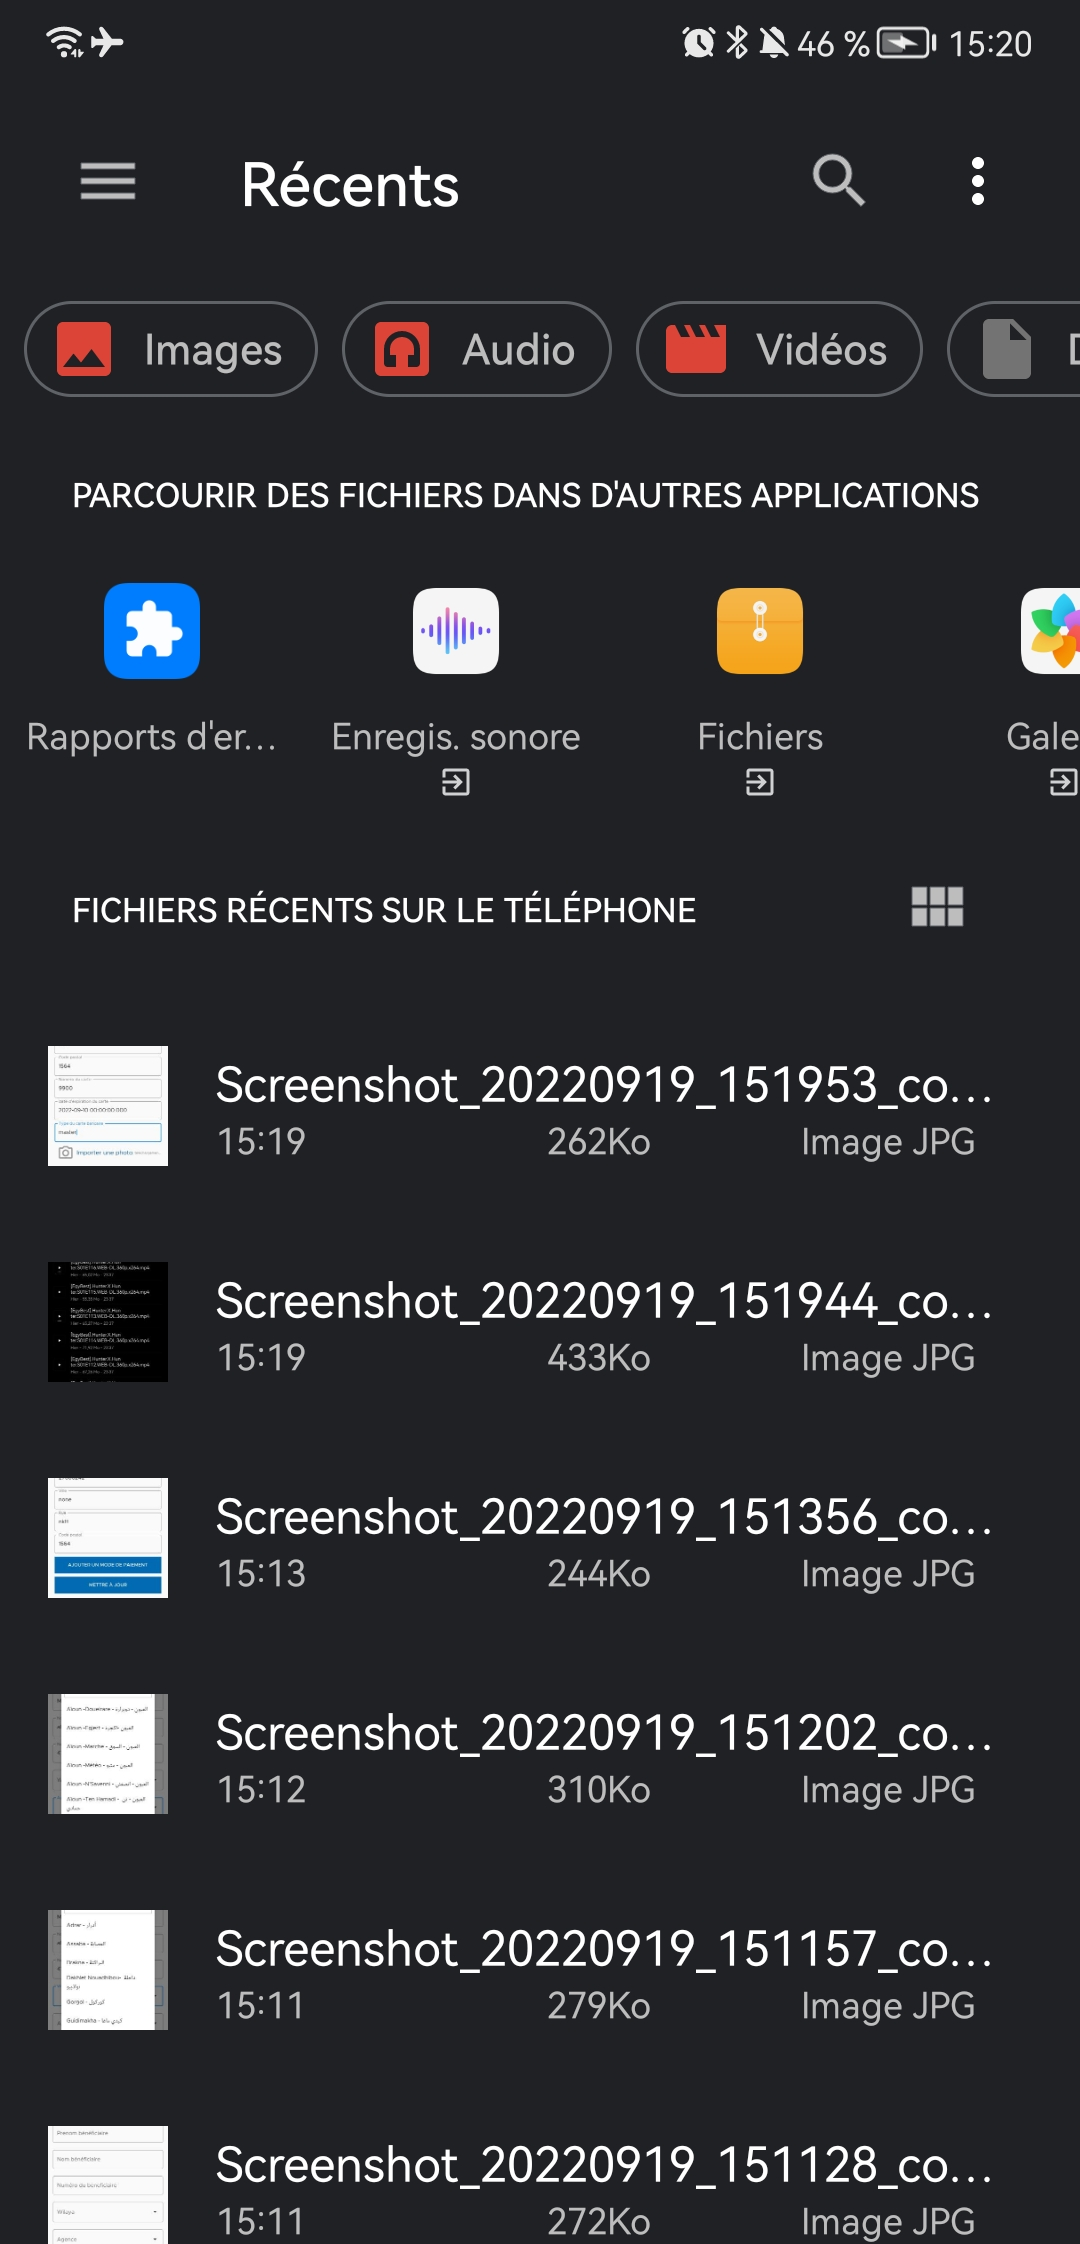
\includegraphics[width=\textwidth]{./Template LaTeX/Images/8.jpg}
		\caption{Mettre à jour un compte}
		\label{fig:five over x}
	\end{subfigure}
	\caption{Interface du compte principal
}
\label{Home}
\end{figure}
\end{comment}
%%%%%%%%%%%%%%%%%%%%%%%%%%%%%%%%%%%%%%%%%%%%%%%%%%%%%%%%%%%%%
\begin{figure}
	\centering
	\begin{subfigure}[b]{0.3\textwidth}
		\centering
		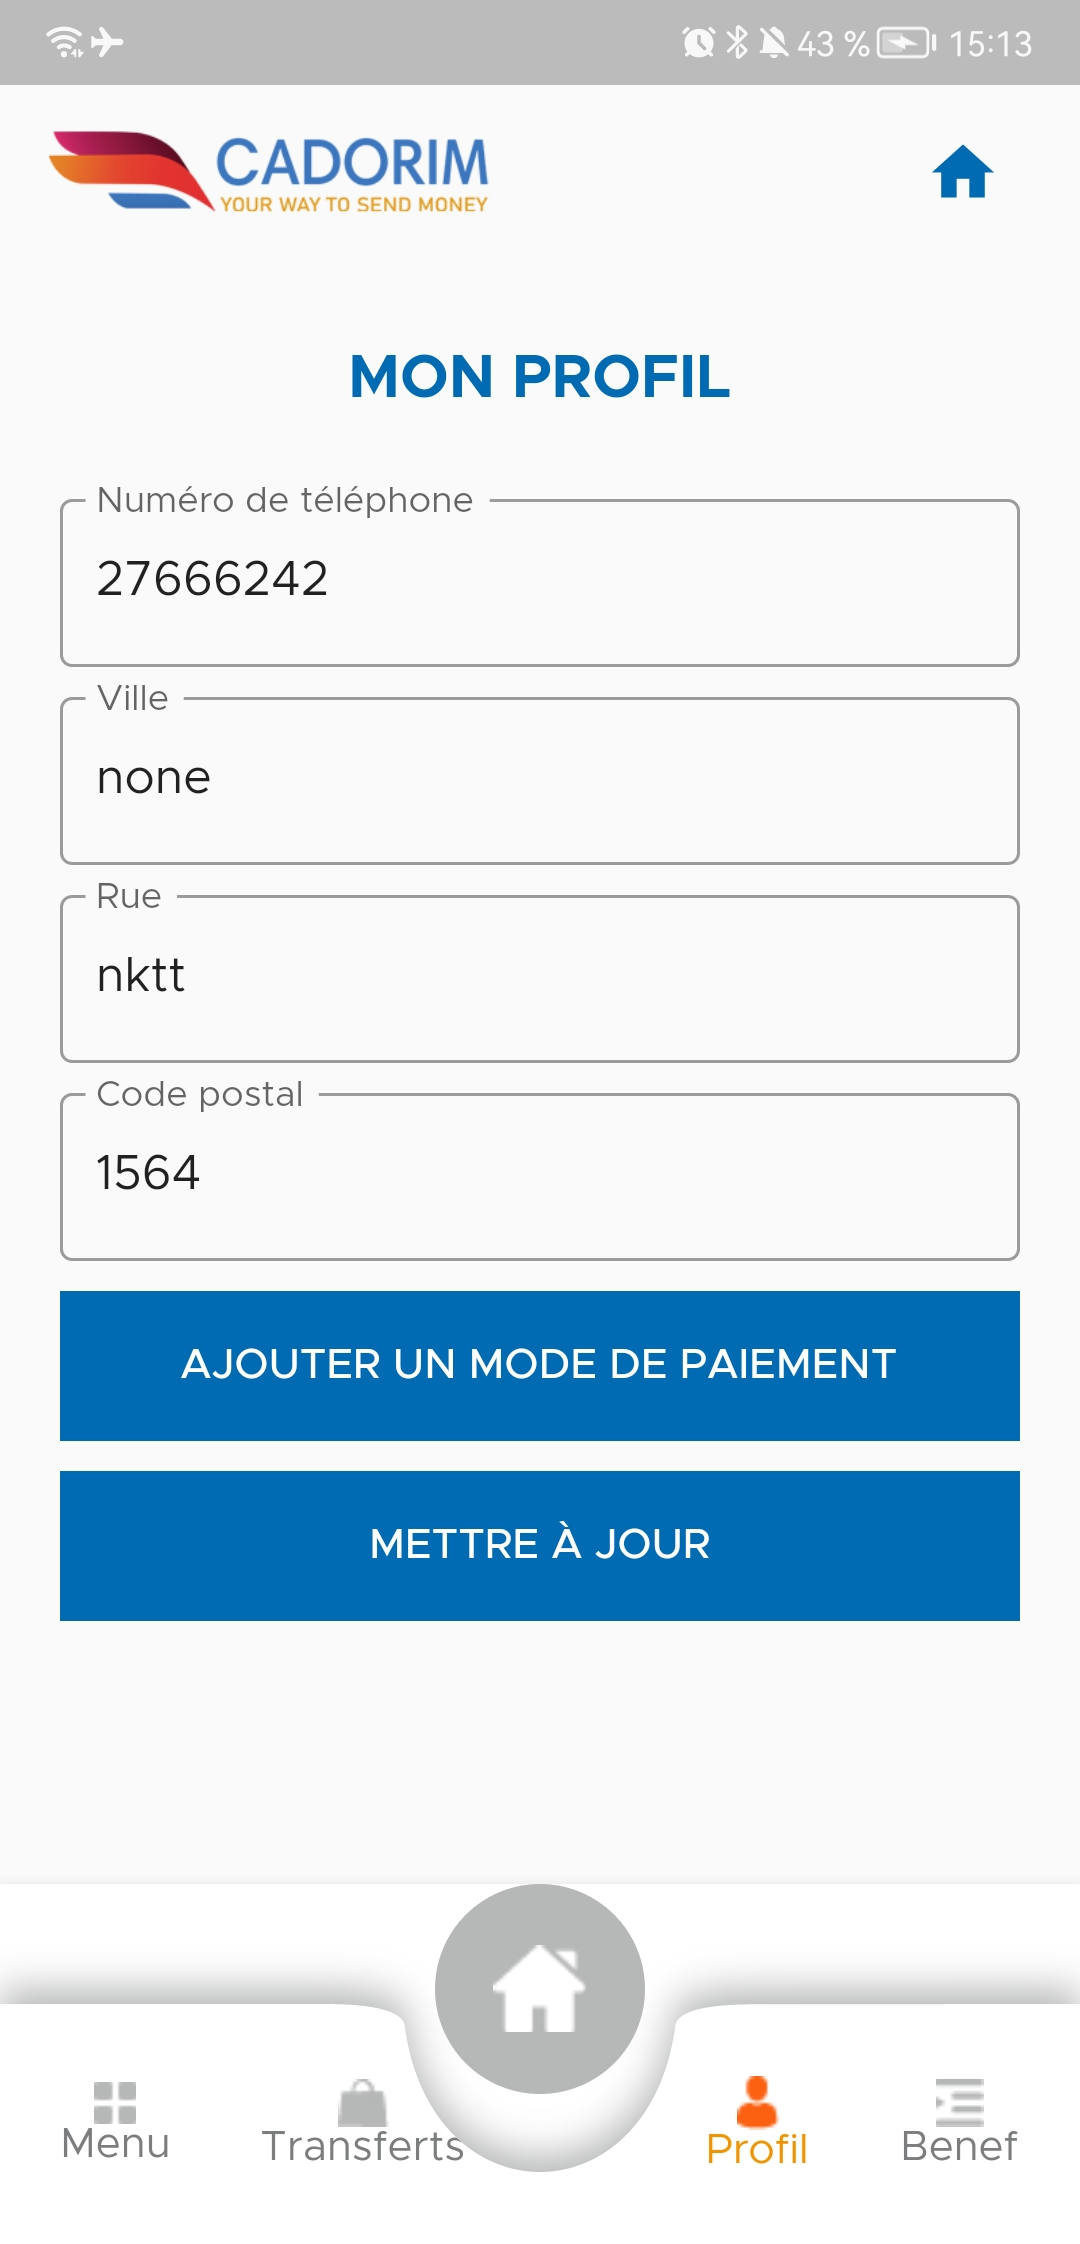
\includegraphics[width=\textwidth]{./Template LaTeX/Images/6.jpg}
		\caption{Interfaces d’accueil}
		\label{fig:y equals x}
	\end{subfigure}
	\hfill
	\begin{subfigure}[b]{0.3\textwidth}
		\centering
		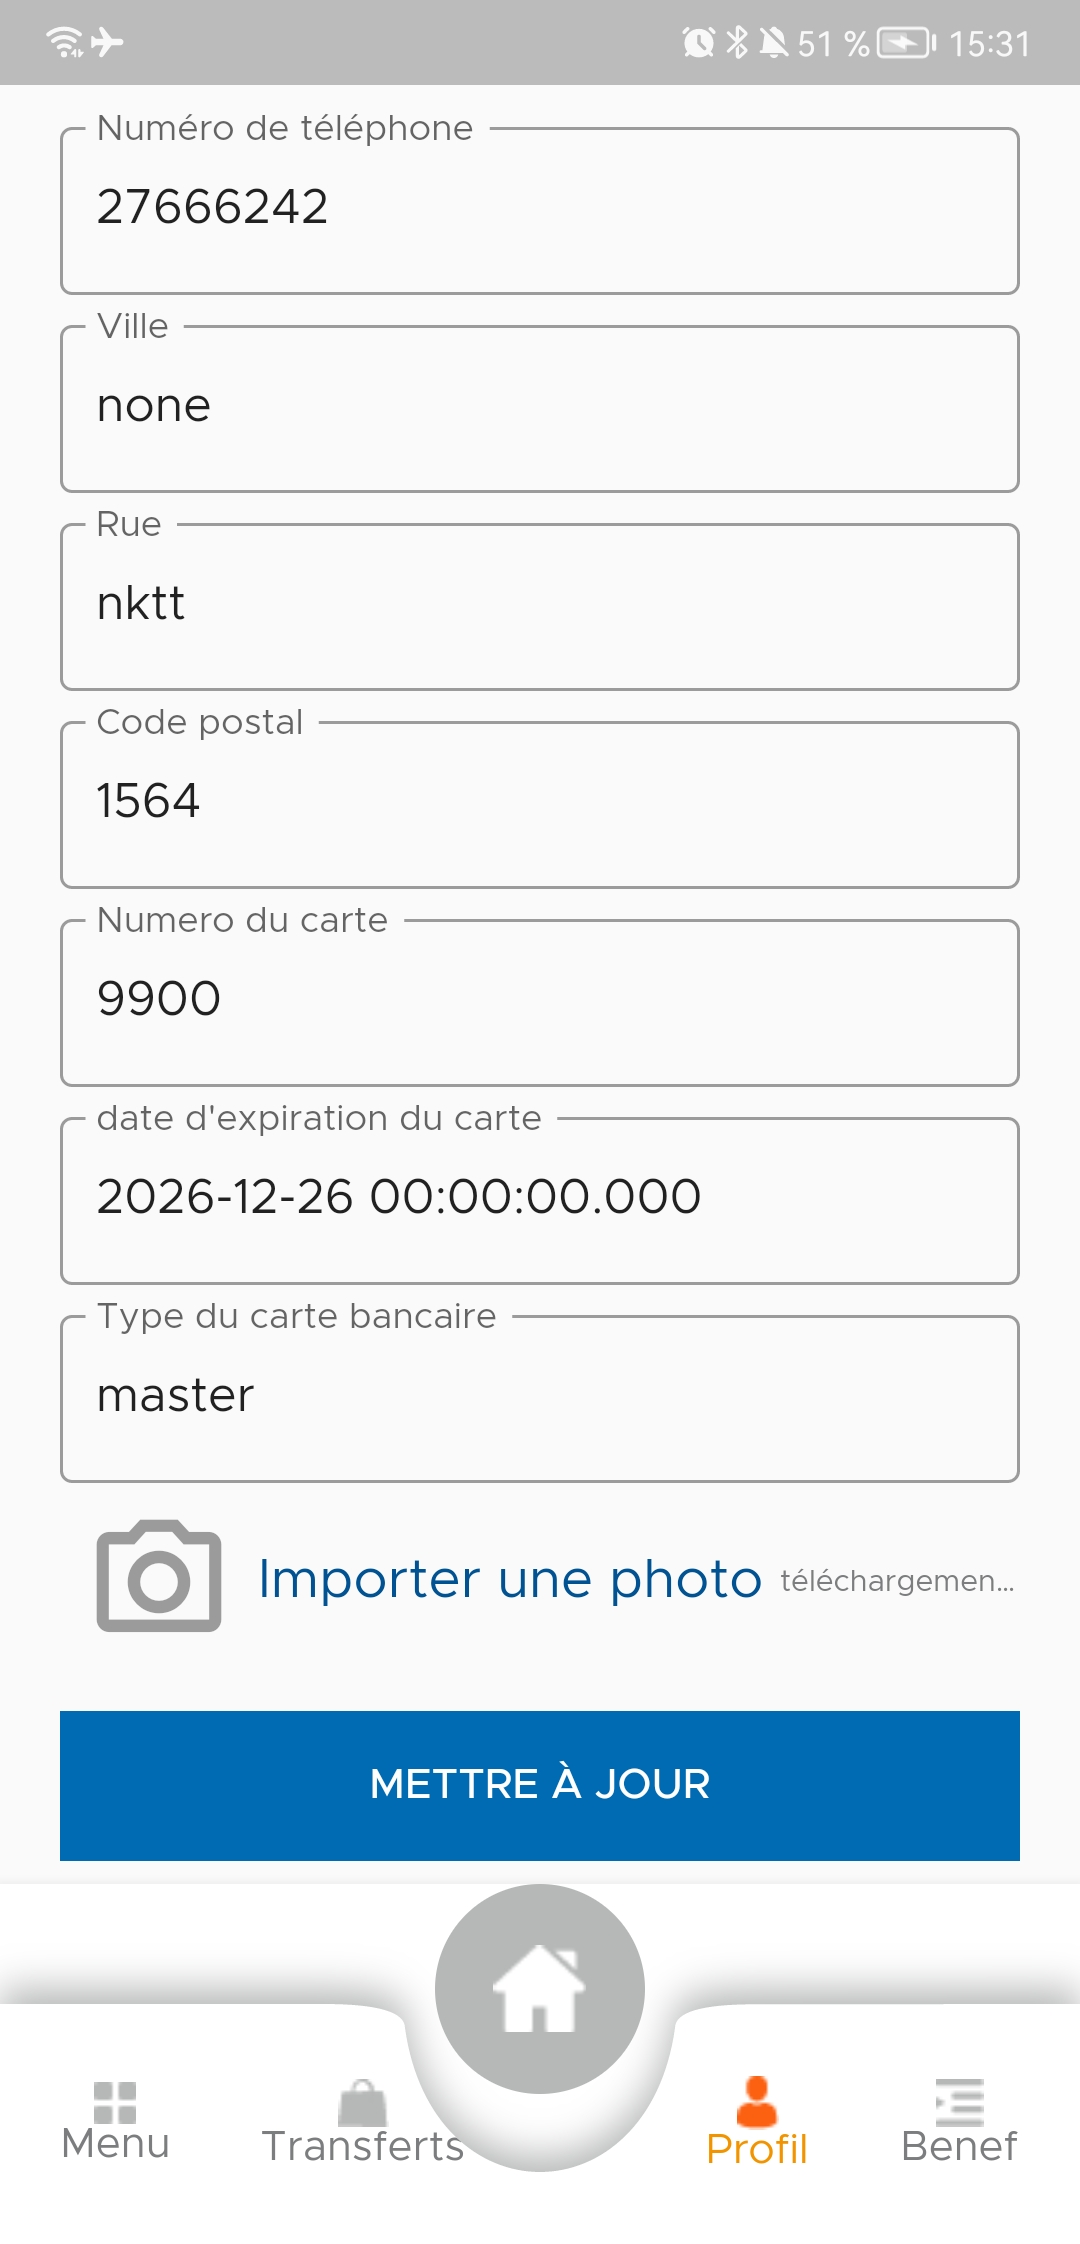
\includegraphics[width=\textwidth]{./Template LaTeX/Images/7.jpg}
		\caption{Gérer un compte}
		\label{fig:three sin x}
	\end{subfigure}
	\hfill
	\begin{subfigure}[b]{0.3\textwidth}
		\centering
		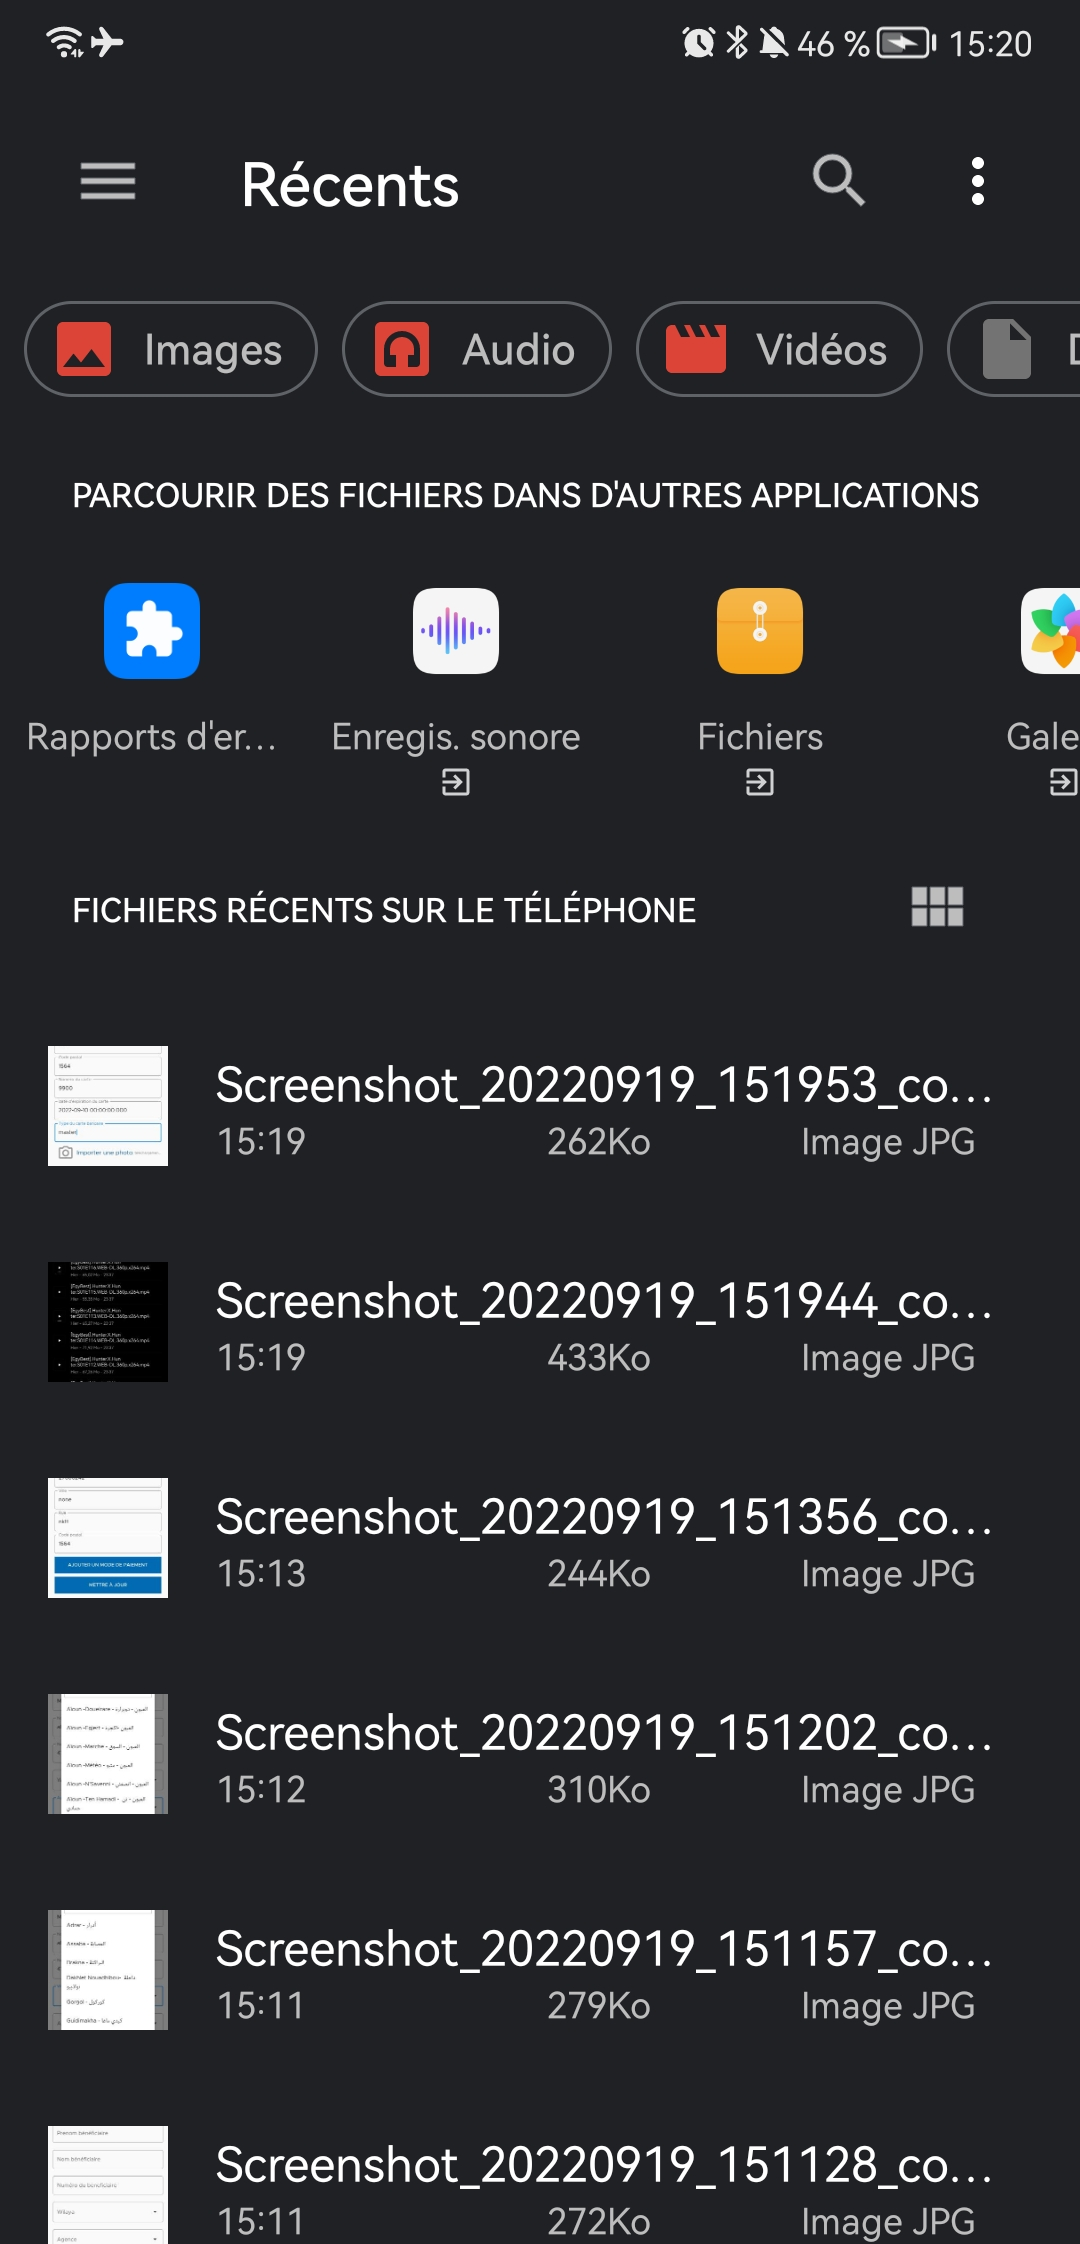
\includegraphics[width=\textwidth]{./Template LaTeX/Images/8.jpg}
		\caption{Mettre à jour un compte}
		\label{fig:five over x}
	\end{subfigure}
	\newline
	\centering
	\begin{subfigure}{0.3\textwidth}
		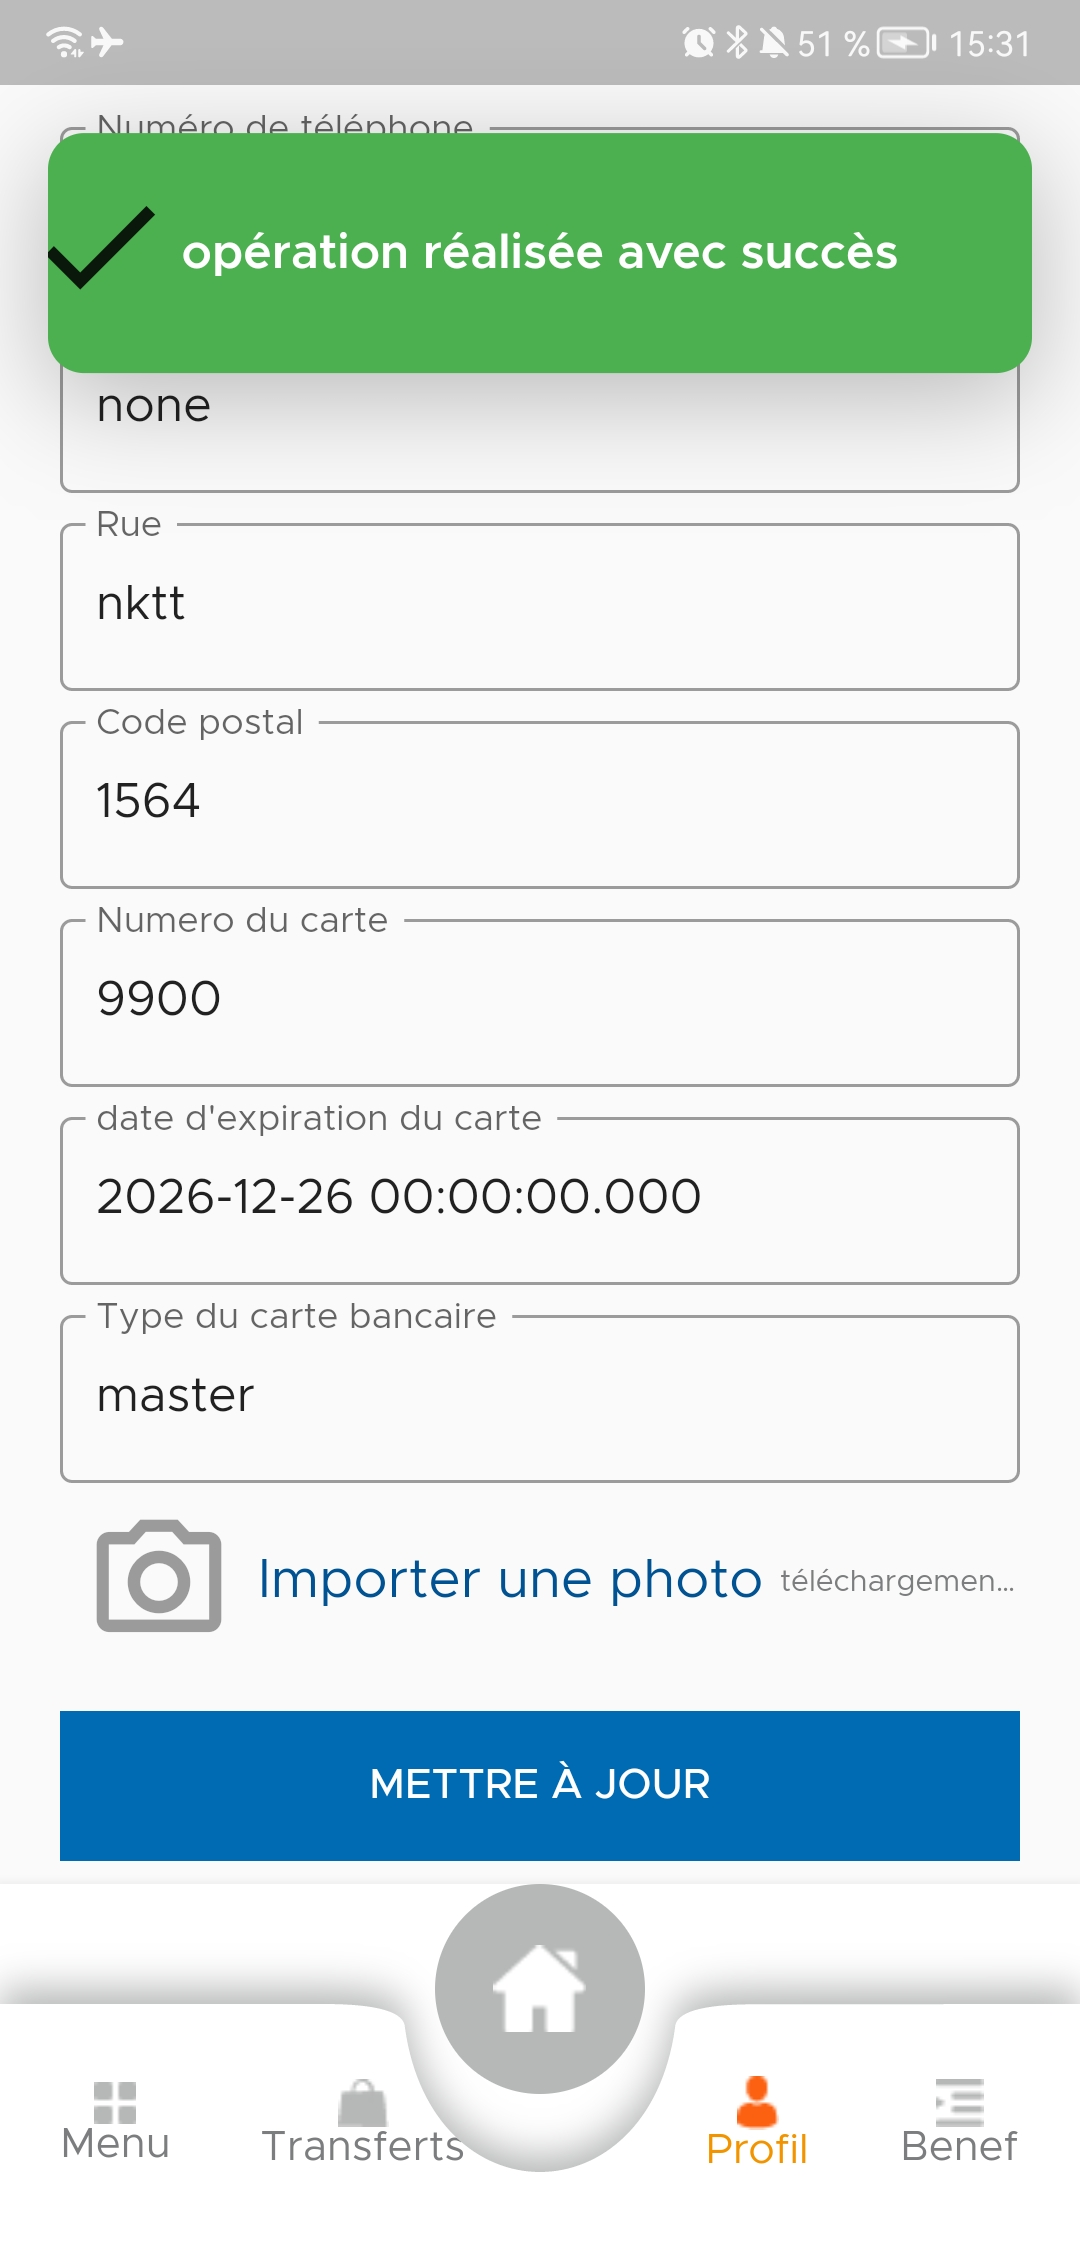
\includegraphics[width=\hsize, valign=m ]{./Template LaTeX/Images/9.jpg}
		\caption{Ajouter un compte}
		\label{fig.SICAPI}
	\end{subfigure}
	%\qquad\tikz[baseline=-\baselineskip]\draw[ultra thick,->] (0,0) -- ++ (1,0);\qquad
	
	\caption{Interface du compte administrateur
}
\label{Home}
\end{figure}
%%%%%%%%%%%%%%%%%%%%%%%%%%%%%%%%%%%%%%%%%%%%%%%%%%%%%%%%%%%%%
\newpage
\item \textbf{L’interface du compte service client
	:} 
La figure~\ref{serviceCl} représente la page principale de l’application pour le compte service client C’est à partir de cette fenêtre l'utilisateur peut répondre aux clients.
\begin{figure}
	\centering
\begin{subfigure}{0.3\textwidth}
	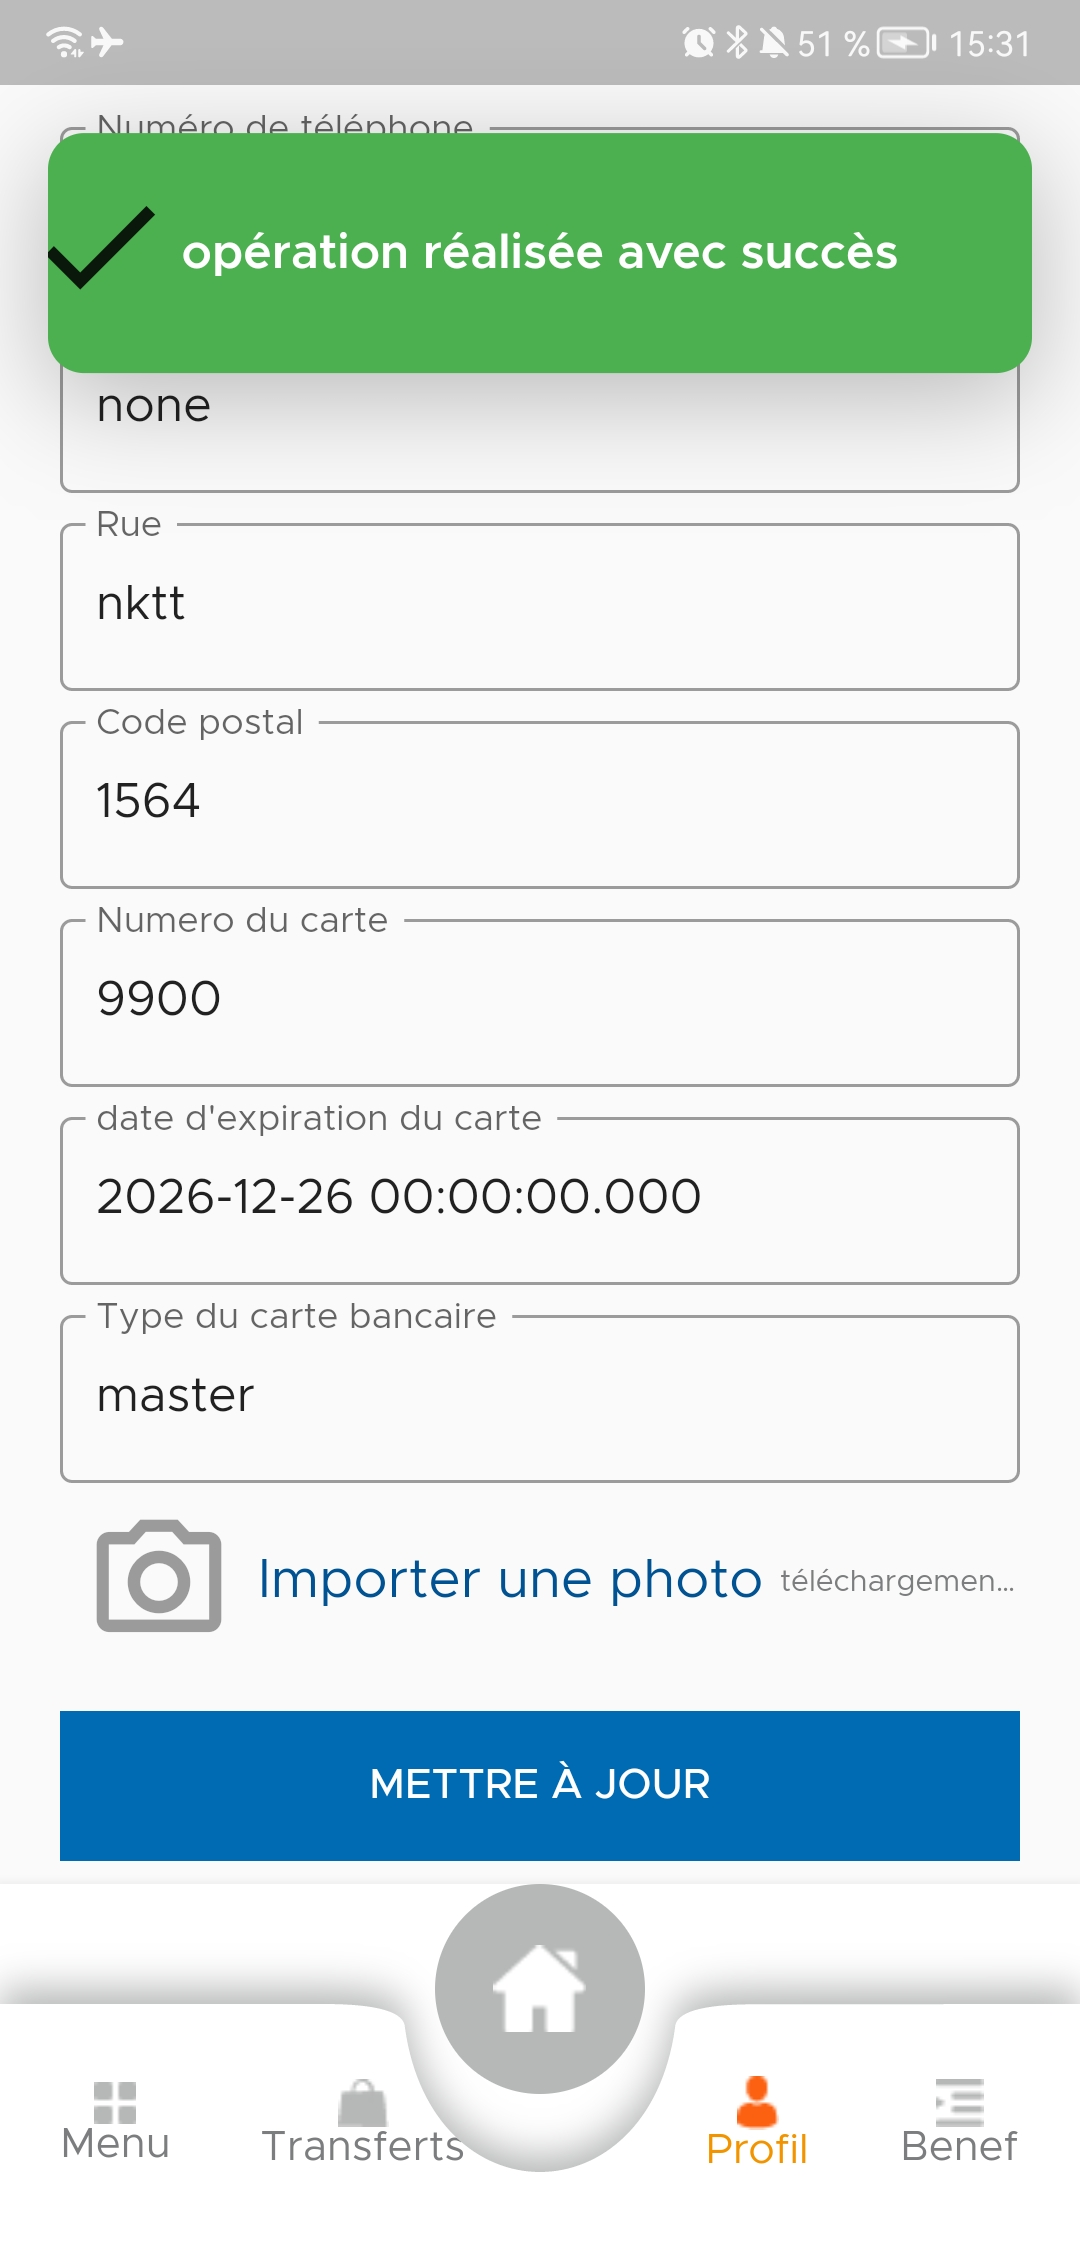
\includegraphics[width=\hsize, valign=m ]{./Template LaTeX/Images/9.jpg}
	\caption{Interfaces d’accueil}
	\label{klk}
\end{subfigure}
\begin{subfigure}{0.3\textwidth}
	\includegraphics[width=\hsize, valign=m ]{./Template LaTeX/Images/20.jpg}
	\caption{Interface de discussion}
	\label{klk}
\end{subfigure}
	\caption{Interface du compte administrateur
}
\label{serviceCl}
\end{figure}
\end{itemize}


